%!TEX root = da-dev.tex

\begin{document}

\frontmatter
\maketitle
\tableofcontents

\uchapter{Foreword}
%!TEX root = da-screen.tex

This online textbook is an introduction to the theory of distributed algorithms. The topics covered in this course include algorithmic techniques that can be used to solve graph problems efficiently in extremely large networks, as well as fundamental impossibility results that put limitations on distributed computing.

No prior knowledge of distributed systems is needed. A basic knowledge of discrete mathematics and graph theory is assumed, as well as familiarity with the basic concepts from undergraduate-level courses on models on computation, computational complexity, and algorithms and data structures.

\paragraph{About the Course.}

This textbook was written to support the lecture course \emph{ICS-E5020 Distributed Algorithms} at Aalto University. The course is worth 5 ETCS credits. There are 12 weeks of lectures: each week there is one 2-hour lecture and one 2-hour exercise session. Each week we will cover roughly one chapter of this book.

Prior versions of this textbook have been used at the course \emph{Deterministic Distributed Algorithms}, which I lectured at the University of Helsinki in 2010, 2012, and 2014.

\paragraph{Acknowledgements.}

Many thanks to Mika G\"o\"os, Juho Hirvonen, Tee\-mu Kuu\-sisto, Tuo\-mo Lem\-pi\"a\-inen, Christoph Lenzen, Stefan Schmid, and Jussi V\"ai\-s\"a\-nen for discussions and comments, and to Juho Hirvonen, Joel Kaasinen, and Joel Rybicki for helping me with the arrangements of this course. This work was supported in part by the Academy of Finland, Grant 252018. For updates and additional material, see
\begin{center}
    \url{http://users.ics.aalto.fi/suomela/da/}
\end{center}

\paragraph{License.}

This work is licensed under the \emph{Creative Commons Attribution--ShareAlike 3.0 Unported License}. To view a copy of this license, visit
\begin{center}
    \url{http://creativecommons.org/licenses/by-sa/3.0/}
\end{center}


\uchapter{Mathematical Preliminaries}\label{ch:math}
%!TEX root = da-dev.tex

In the analysis of distributed algorithms, we will sometimes encounter power towers and iterated logarithms.


\usection{Power Tower}

We write power towers with the notation
\[
    {}^i 2 = 2^{2^{\cdot^{\cdot^2}}},
\]
where there are $i$ twos in the tower. Power towers grow very fast; for example,
\begin{align*}
    {}^1 2 &= 2,\\
    {}^2 2 &= 4,\\
    {}^3 2 &= 16,\\
    {}^4 2 &= 65536,\\
    {}^5 2 &= 2^{65536} > 10^{19728}.
\end{align*}


\usection{Iterated Logarithm}

The iterated logarithm of $x$, in notation $\log^* x$, is defined recursively as follows:
\[
    \log^*(x) = \begin{cases}
        0 & \text{ if $x \le 1$}, \\
        1 + \log^*(\log_2 x) & \text{ otherwise}.
    \end{cases}
\]
In essence, this is the inverse of the power tower function. For all positive integers $i$, we have
\[
    \log^* {}^i 2 = i.
\]
As power towers grow very fast, iterated logarithms grow very slowly; for example,
\begin{align*}
    \log^* 2 &= 1, &
    \log^* 16 &= 3, &
    \log^* 10^{10} &= 5, \\
    \log^* 3 &= 2, &
    \log^* 17 &= 4, &
    \log^* 10^{100} &= 5, \\
    \log^* 4 &= 2, &
    \log^* 65536 &= 4, &
    \log^* 10^{1000} &= 5, \\
    \log^* 5 &= 3, &
    \log^* 65537 &= 5, &
    \log^* 10^{10000} &= 5, \dotsc
\end{align*}


\mainmatter
\part{Informal Introduction}

\chapter{Warm-Up\mydash Positive Results}\label{ch:intro-pos}
%!TEX root = da-screen.tex

We will start this book with an informal introduction to distributed algorithms. We will formalise the model of computing later, starting with some graph-theoretic preliminaries in Chapter~\ref{ch:graphs}, and then followed by the definitions of three models of distributed computing in Chapters \ref{ch:pn}--\ref{ch:congest}. However, in the first two chapters the intuitive idea of computers that can exchange messages with each others is sufficient.

\section{Running Example: Colouring Paths}

Imagine that we have $n$ computers (or \emph{nodes} as they are usually called) that are connected to each other with communication channels so that the network topology is a \emph{path}:
\begin{center}
    \includegraphics[page=\PIntroTopo]{figs.pdf}
\end{center}
The computers can exchange messages with their neighbours. All computers run the \emph{same} algorithm\mydash this is the \emph{distributed algorithm} that we will design. The algorithm will decide what messages a computer sends in each step, how it processes the messages that it receives, when it stops, and what it outputs when it stops.

In this example, the task is to find a proper \emph{colouring} of the path with $3$ colours. That is, each node has to output one of the colours, $1$, $2$, or $3$, so that neighbours have different colours\mydash here is an example of a proper solution:
\begin{center}
    \includegraphics[page=\PIntroCol]{figs.pdf}
\end{center}

\section{Challenges of Distributed Algorithm}\label{sec:intro-challenges}

With a bird's-eye view of the entire network, colouring a path looks like a very simple task: just start from one endpoint and assign colours $1$ and $2$ alternately. However, in a real-world computer network we usually do not have all-powerful entities that know everything about the network and can directly tell each computer what to do.

Indeed, when we start a networked computer, it is typically only aware of itself and the communication channels that it can use. In our simple example, the endpoints of the path know that they have one neighbour:
\begin{center}
    \includegraphics[page=\PIntroDegOne]{figs.pdf}
\end{center}
All other nodes along the path just know that they have two neighbours:
\begin{center}
    \includegraphics[page=\PIntroDegTwo]{figs.pdf}
\end{center}
For example, the second node along the path looks no different from the third node, yet somehow they have to produce \emph{different} outputs.

Obviously, the nodes have to exchange \emph{messages} with each other in order to figure out a proper solution. Yet this turns out to be surprisingly difficult even in the case of just $n = 2$ nodes:
\begin{center}
    \includegraphics[page=\PIntroTwo]{figs.pdf}
\end{center}
If we have two \emph{identical} computers connected to each other with a single communication link, both computers are started simultaneously, and both of them run the same deterministic algorithm, how could they ever end up in \emph{different} states?

The answer is that it is not possible, without some additional assumptions. In practice, we could try to rely on some real-world imperfections (e.g., the computers are seldom perfectly synchronised), but in the theory of distributed algorithms we often assume that there is some \emph{explicit} way to \emph{break symmetry} between otherwise identical computers. In this chapter, we will have a brief look at two common assumption:
\begin{itemize}[noitemsep]
    \item each computer has a unique name,
    \item each computer has a source of random bits.
\end{itemize}
In subsequent chapters we will then formalise these models, and develop a theory that will help us understand precisely what kind of tasks can be solved in each case, and how fast (the model with unique names will be discussed in detail in Chapter~\ref{ch:local}, and randomised algorithms will be discussed in Chapter~\ref{ch:rand}).


\section{Colouring with Unique Identifiers}\label{sec:algo-p3c}

There are plenty of examples of real-world networks with globally unique identifiers: public IPv4 and IPv6 addresses are globally unique identifiers of Internet hosts, devices connected to an Ethernet network have globally unique MAC addresses, mobile phones have their IMEI numbers, etc. The common theme is that the identifiers are globally unique, and the numbers can be interpreted as natural numbers:
\begin{center}
    \includegraphics[page=\PIntroId]{figs.pdf}
\end{center}
With the help of unique identifiers, it is now easy to design an algorithm that colours a path. Indeed, the unique identifiers already form a colouring with a large number of colours! All that we need to do is to reduce the number of colours to $3$.

We can use the following simple strategy. In each step, a node is active if it is a ``local maximum'', i.e., its current colour is larger than the current colours of its neighbours:
\begin{center}
    \includegraphics[page=\PIntroIdA]{figs.pdf}
\end{center}
The active nodes will then pick a new colour from the colour palette $\{1,2,3\}$, so that it does not conflict with the current colours of their neighbours. This is always possible, as each node in a path has at most $2$ neighbours, and we have $3$ colours in our colour palette:
\begin{center}
    \includegraphics[page=\PIntroIdAA]{figs.pdf}
\end{center}
Then we simply repeat the same procedure until all nodes have small colours. First find the local maxima:
\begin{center}
    \includegraphics[page=\PIntroIdB]{figs.pdf}
\end{center}
And then recolour the local maxima with colours from $\{1,2,3\}$:
\begin{center}
    \includegraphics[page=\PIntroIdBB]{figs.pdf}
\end{center}
Continuing this way we will eventually have a path that is properly coloured with colours $\{1,2,3\}$:
\begin{center}
    \includegraphics[page=\PIntroIdC]{figs.pdf}\\
    \includegraphics[page=\PIntroIdCC]{figs.pdf}\\
    \includegraphics[page=\PIntroIdD]{figs.pdf}\\
    \includegraphics[page=\PIntroIdDD]{figs.pdf}\\
    \includegraphics[page=\PIntroIdE]{figs.pdf}\\
    \includegraphics[page=\PIntroIdEE]{figs.pdf}
\end{center}
Note that we may indeed be forced to use all three colours.

So far we have sketched an algorithm idea, but we still have to show that we can actually implement this idea as a distributed algorithm. Remember that there is no central control; nobody has a bird's-eye view of the entire network. Each node is an independent computer, and all computers are running the \emph{same} algorithm. What would the algorithm look like?

Let us fix some notation. Each node maintains a variable $c$ that contains its current colour. Initially, $c$ is equal to the unique identifier of the node. Then computation proceeds as shown in Table~\ref{tab:algo-p3c}; we will call this algorithm $\algo{P3C}$.

\begin{table}
    \raggedright
    \algtoprule
    \begin{descriptionb}
        \item[Repeat forever:] \mbox{}
        \begin{itemize}
            \item Send message $c$ to all neighbours.
            \item Receive messages from all neighbours. \\
                  Let $M$ be the set of messages received.
            \item If $c \notin \{1,2,3\}$ and $c > \max M$: \\
                  Let $c \gets \min\,(\{1,2,3\} \setminus M)$.
        \end{itemize}
    \end{descriptionb}
    \algbottomrule
    \caption{Algorithm $\algo{P3C}$: $3$-colouring a path.}\label{tab:algo-p3c}
\end{table}

This shows a typical structure of a distributed algorithm: an infinite send--receive--compute loop. A computer is seen as a state machine; here $c$ is the variable that holds the current state of the computer. In this algorithm, we have three \emph{stopping states}: $c = 1$, $c = 2$, and $c = 3$. It is easy to verify that the algorithm is indeed correct in the following sense:
\begin{enumerate}
    \item In any path graph, for any assignment of unique identifiers, all computers will eventually reach a stopping state.
    \item Once a computer reaches a stopping state, it never changes its state.
\end{enumerate}
The second property is very important: each computer has to know when it is safe to announce its output and stop.

Our algorithm may look a bit strange in the sense that computers that have ``stopped'' are still sending messages. However, it is fairly straightforward to rewrite the algorithm so that you could actually turn off computers that have stopped. The basic idea is that nodes that are going to switch to a stopping state first inform their neighbours about this. Each node will memorise which of its neighbours have already stopped and what where their final colours. Implementing this idea is left as Exercise~\ref{ex:intro-stopped}, and you will later see in Chapter~\ref{ch:pn} that this can be done for \emph{any} distributed algorithm. Hence, without loss of generality, we can play by the following simple rules:
\begin{itemize}
    \item The nodes are state machines that repeatedly send messages to their neighbours, receive messages from their neighbours, and update their state\mydash all nodes perform these steps synchronously in parallel.
    \item Some of the states are stopping states, and once a node reaches a stopping state, its no longer changes its state.
    \item Eventually all nodes have to reach stopping states, and these states must form a correct solution to the problem that we want to solve.
\end{itemize}
Note that here a ``state machine'' does not necessarily refer to a \emph{finite}-state machine. We can perfectly well have a state machine with infinitely many states. Indeed, in the example of Table~\ref{tab:algo-p3c} the set of possible states was the set of all positive integers.


\section{Faster Colouring with Unique Identifiers}\label{sec:algo-p3cbit}

So far we have seen that with the help of unique identifiers, it is \emph{possible} to find a $3$-colouring of a path. However, the algorithm that we designed is not particularly efficient in the worst case. To see this, consider a path in which the unique identifiers happen to be assigned in an increasing order:
\begin{center}
    \includegraphics[page=\PIntroIdBad]{figs.pdf}
\end{center}
In such a graph, in each round there is only one node that is active. In total, it will take $\Theta(n)$ rounds until all nodes have stopped.

However, it is possible to colour paths \emph{much} faster. The algorithm is easier to explains if we have a \emph{directed} path:
\begin{center}
    \includegraphics[page=\PIntroIdDir]{figs.pdf}
\end{center}
That is, we have a consistent orientation in the path so that each node has at most one ``predecessor'' and at most one ``successor''. The orientations are just additional information that we will use in algorithm design\mydash nodes can always exchange information along each edge in either direction. Once we have presented the algorithm for directed paths, we will then generalise it to undirected paths in Exercise~\ref{ex:intro-undir-path}.


\subsection{Algorithm Overview}

For the sake of concreteness, let us assume that the nodes are labelled with $128$-bit unique identifiers\mydash for example, IPv6 addresses. In most real-world networks $2^{128}$ identifiers is certainly more than enough, but the same idea can be easily generalised to arbitrarily large identifiers if needed.

Again, we will interpret the unique identifiers as colours; hence our starting point is a path that is properly coloured with $2^{128}$ colours. In the next section, we will present algorithm called $\algo{P3CBit}$ that reduces the number of colours from $2^x$ to $2x$ in one round, for any positive integer $x$. Hence in one step we can reduce the number of colours from $2^{128}$ to $2 \cdot 128 = 256$. In just four iterations we can reduce the number of colours from $2^{128}$ to $6$, as follows:
\begin{align*}
    2^{128} &\to 2 \cdot 128 = 2^8, \\
    2^8 &\to 2 \cdot 8 = 2^4, \\
    2^4 &\to 2 \cdot 4 = 2^3, \\
    2^3 &\to 2 \cdot 3 = 6.
\end{align*}
Once we have found a $6$-colouring, we can then apply the algorithm of Table~\ref{tab:algo-p3c} to reduce the number of colours from $6$ to $3$. It is easy to see that this will take at most $3$ rounds. Overall, we have an algorithm that reduces the number of colours from $2^{128}$ to $3$ in only $7$ rounds\mydash no matter how many nodes we have in the path. Compare this with algorithm $\algo{P3C}$, which may take millions of rounds for paths with millions of nodes.


\subsection{Algorithm for One Step}

Let us now show how algorithm $\algo{P3CBit}$ reduces the number of colours from $2^x$ to $2x$ in one round; as the name suggests, we will be doing some bit manipulations here. First, each node sends its current colour to its predecessor. After this step, each node $u$ knows two values:
\begin{itemize}[noitemsep]
    \item $c_0(u)$, the current colour of the node,
    \item $c_1(u)$, the current colour of its successor.
\end{itemize}
If a node does not have any successor, it just proceeds \emph{as if} it had a successor of some colour different from $c_0(u)$.

We can interpret both $c_0(u)$ and $c_1(u)$ as $x$-bit binary strings that represent integers from range $0$ to $2^x-1$. We know that the current colour of node $u$ is different from the current colour of its successor, i.e., $c_0(u) \ne c_1(u)$. Hence in the two binary strings $c_0(u)$ and $c_1(u)$ there is at least one bit that differs. Define:
\begin{itemize}
    \item $i(u) \in \{0,1,\dotsc,x-1\}$ is the \emph{\textbf{index}} of the first bit that differs between $c_0(u)$ and $c_1(u)$,
    \item $b(u) \in \{0,1\}$ is the \emph{\textbf{value}} of bit number $i(u)$ in $c_0(u)$.
\end{itemize}
Finally, node $u$ chooses
\[
    c(u) = 2i(u) + b(u)
\]
as its new colour.


\begin{table}
    \newcommand{\hl}[1]{\mathbf{\color{hlcolor}#1}}
    \newcommand{\node}{\raisebox{-1pt}{$\bigcirc$}}
    \newcommand{\mylf}{\\[-2pt]}
    \center
    \begin{tabular}{@{}c@{\qquad}ccccc@{}}
    \toprule
    node & input &&&& output \\
    $u$ & $c_0(u)$ & $c_1(u)$ & $i(u)$ & $b(u)$ & $c(u)$ \\
    \midrule
    $\cdots$ & $\cdots$ & $\cdots$ & $\cdots$ & $\cdots$ & $\cdots$ \mylf
    $\downarrow$ \mylf
    \node & $01111\hl{0}11_2$ & $00101\hl{1}11_2$ & $2$ & $0$ & $4$ \mylf
    $\downarrow$ \mylf
    \node & $00101\hl{1}11_2$ & $01101\hl{0}11_2$ & $2$ & $1$ & $5$ \mylf
    $\downarrow$ \mylf
    $\node$ & $01101011_2$ & $\cdots$ & $\cdots$ & $\cdots$ & $\cdots$ \mylf
    $\downarrow$ \mylf
    $\cdots$ & $\cdots$ \mylf
    \midrule
    $\cdots$ & $\cdots$ & $\cdots$ & $\cdots$ & $\cdots$ & $\cdots$ \mylf
    $\downarrow$ \mylf
    \node & $01111\hl{0}11_2$ & $00101\hl{1}11_2$ & $2$ & $0$ & $4$ \mylf
    $\downarrow$ \mylf
    \node & $0\hl{0}101111_2$ & $0\hl{1}101111_2$ & $6$ & $0$ & $12$ \mylf
    $\downarrow$ \mylf
    $\node$ & $01101111_2$ & $\cdots$ & $\cdots$ & $\cdots$ & $\cdots$ \mylf
    $\downarrow$ \mylf
    $\cdots$ & $\cdots$ \mylf
    \bottomrule
    \end{tabular}
    \caption{Algorithm $\algo{P3CBit}$: reducing the number of colours from $2^x$ to $2x$, for $x = 8$. There are two interesting cases: either $i(u)$ is the same for two neighbours (first example), or they are different (second example). In the first case, the values $b(u)$ will differ, and in the second case, the values $i(u)$ will differ. In both cases, the final colours $c(u)$ will be different.}\label{tab:algo-p3cbit}
\end{table}


\subsection{An Example}

Let $x = 8$, i.e., nodes are coloured with $8$-bit numbers. Assume that we have a node $u$ of colour $123$, and $u$ has a successor $v$ of colour $47$; see Table~\ref{tab:algo-p3cbit} for an illustration. In binary, we have
\begin{align*}
    c_0(u) &= 01111011_2, \\
    c_1(u) &= 00101111_2.
\end{align*}
\begin{samepage}
Counting from the least significant bit, node $u$ can see that:
\begin{itemize}[noitemsep]
    \item bit number $0$ is the same in both $c_0(u)$ and $c_1(u)$,
    \item bit number $1$ is the same in both $c_0(u)$ and $c_1(u)$,
    \item bit number $2$ is different in $c_0(u)$ and $c_1(u)$.
\end{itemize}
\end{samepage}
Hence we will set
\[
    i(u) = 2, \quad
    b(u) = 0, \quad
    c(u) = 2\cdot2 + 0 = 4.
\]
That is, node picks $4$ as its new colour. If all other nodes run the same algorithm, this will be a valid choice\mydash as we will argue next, both the predecessor and the successor of $u$ will pick a colour that is different from $4$.


\subsection{Correctness}

Clearly, the value $c(u)$ is in the range $\{0,1,\dotsc,2x-1\}$. However, it is not entirely obvious that these values actually produce a proper $2x$-colouring of the path. To see this, consider a pair of nodes $u$ and $v$ so that $v$ is the successor of $u$. By definition, $c_1(u) = c_0(v)$. We need to show that $c(u) \ne c(v)$. There are two cases\mydash see Table~\ref{tab:algo-p3cbit} for an example:
\begin{enumerate}
    \item $i(u) = i(v) = i$: We know that $b(u)$ is bit number $i$ of $c_0(u)$, and $b(v)$ is bit number $i$ of $c_1(u)$. By the definition of $i(u)$, we also know that these bits differ. Hence $b(u) \ne b(v)$ and $c(u) \ne c(v)$.
    \item $i(u) \ne i(v)$: No matter how we choose $b(u) \in \{0,1\}$ and $b(v) \in \{0,1\}$, we have $c(u) \ne c(v)$.
\end{enumerate}
We have argued that $c(u) \ne c(v)$ for any pair of two adjacent nodes $u$ and $v$, and the value of $c(u)$ is an integer between $0$ and $2x-1$ for each node $u$. Hence the algorithm finds a proper $2x$-colouring in one round.


\subsection{Iteration}

The algorithm that we presented in this chapter can reduce the number of colours from $2^x$ to $2x$ in one round; put otherwise, we can reduce the number of colours from $x$ to $O(\log x)$ in one round.

If we iterate the algorithm, we can reduce the number of colours from $x$ to $6$ in $O(\log^* x)$ rounds, after which we can use algorithm $\algo{P3C}$ from Section~\ref{sec:algo-p3c} to reduce the number of colours from $6$ to $3$ in $3$ rounds\mydash the details of the analysis are left as Exercises \ref{ex:logstar} and~\ref{ex:logstar-tight}.


\section{Colouring with Randomised Algorithms}\label{sec:algo-p3crand}

So far we have used unique identifiers to break symmetry. Another possibility is to use randomness. Here is a simple randomised distributed algorithm that finds a proper $3$-colouring of a path: nodes try to pick colours from the palette $\{1,2,3\}$ uniformly at random, and they stop once they succeed in picking a colour that is different from the colours of their neighbours.


\subsection{Algorithm}

Let us formalise the algorithm that we sketched above; we will call this algorithm $\algo{P3CRand}$. Each node $u$ has a flag $s(u) \in \{0,1\}$ indicating whether it has stopped, and a variable $c(u) \in \{1,2,3\}$ that stores its current colour. If $s(u) = 1$, a node has stopped and its output is $c(u)$.

In each step, each node $u$ with $s(u) = 0$ picks a new colour $c(u) \in \{1,2,3\}$ uniformly at random. Then each node sends its current colour $c(u)$ to its neighbours. If $c(u)$ is different from the colours of its neighbours, $u$ will set $s(u) = 1$ and stop; otherwise it tries again in the next round.


\subsection{Analysis}

It is easy to see that in each step, a node $u$ will stop with probability at least $1/3$: after all, no matter what its neighbours do, there is at least one choice for $c(u) \in \{1,2,3\}$ that does not conflict with its neighbours.

Fix a positive constant $C$. Consider what happens if we run the algorithm for
\[
    k = (C+1) \log_{3/2} n
\]
steps, where $n$ is the number of nodes in the network. Now the probability that a given node $u$ has not stopped after $k$ steps is at most
\[
    (1 - 1/3)^k = \frac{1}{n^{C+1}}.
\]
By the union bound, the probability that there is a node that has not stopped is at most $1/n^C$. Hence with probability at least $1-1/n^C$, all nodes have stopped after $k$ steps.


\subsection{With High Probability}

Let us summarise what we have achieved: for any given constant $C$, there is an algorithm that runs for $k = O(\log n)$ rounds and produces a proper $3$-colouring of a path with probability $1-1/n^C$. We say that the algorithm runs in time $O(\log n)$ \emph{with high probability}\mydash here the phrase ``high probability'' means that we can choose any constant $C$ and the algorithm will succeed at least with a probability of $1-1/n^C$. Note that even for a moderate value of $C$, say, $C = 10$, the success probability approaches $1$ very rapidly as $n$ increases.


\section{Summary}

In this chapter we have seen three different distributed algorithms for $3$-colouring paths:
\begin{itemize}
    \item Algorithm $\algo{P3C}$, Section~\ref{sec:algo-p3c}: A deterministic algorithm for paths with unique unique identifiers. Runs in $O(n)$ rounds, where $n$ is the number of nodes.
    \item Algorithm $\algo{P3CBit}$, Section~\ref{sec:algo-p3cbit}: A deterministic algorithm for \emph{directed} paths with unique unique identifiers. Runs in $O(\log^* x)$ rounds, where $x$ is the largest identifier.
    \item Algorithm $\algo{P3CRand}$, Section~\ref{sec:algo-p3crand}: A randomised algorithm for paths without unique identifiers. Runs in $O(\log n)$ rounds with high probability.
\end{itemize}
We will explore and analyse these algorithms and their variants in more depth in the exercises.


\section{Exercises}

\begin{ex}[maximal independent sets]\label{ex:intro-mis}
    A \emph{maximal independent set} is a set of nodes $I$ that satisfies the following properties:
    \begin{itemize}[noitemsep]
        \item for each node $v \in I$, none of its neighbours are in $I$,
        \item for each node $v \notin I$, at least one of its neighbours is in $I$.
    \end{itemize}
    Here is an example\mydash the nodes labelled with a ``1'' form a maximal independent set:
    \begin{center}
        \includegraphics[page=\PIntroMis]{figs.pdf}
    \end{center}
    Your task is to design a distributed algorithm that finds a maximal independent set in any path graph, for each of the following settings:
    \begin{subex}
        \item\label{subex:intro-mis-a} a deterministic algorithm for paths with arbitrarily large unique unique identifiers,
        \item\label{subex:intro-mis-b} a fast deterministic algorithm for \emph{directed} paths with $128$-bit unique identifiers,
        \item\label{subex:intro-mis-c} a randomised algorithm that does not need unique identifiers. 
    \end{subex}
    In part \ref{subex:intro-mis-a}, use the techniques presented in Section~\ref{sec:algo-p3c},
    in part \ref{subex:intro-mis-b}, use the techniques presented in Section~\ref{sec:algo-p3cbit}, and
    in part \ref{subex:intro-mis-c}, use the techniques presented in Section~\ref{sec:algo-p3crand}.
\end{ex}

\begin{ex}[stopped nodes]\label{ex:intro-stopped}
    Rewrite the greedy algorithm of Table~\ref{tab:algo-p3c} so that stopped nodes do not need to send messages. Be precise: explain your algorithm in detail so that you could easily implement it.
\end{ex}

\begin{ex}[undirected paths]\label{ex:intro-undir-path}
    Algorithm $\algo{P3CBit}$ finds a $3$-colouring very fast in any directed path. Design an algorithm that is almost as fast and works in any path, even if the edges are not directed.

    \hint{Use the local maxima and minima to partition the path in subpaths so that within each subpath we have unique identifiers given in an increasing order. Use this ordering to orient each subpath. Then we can apply the fast colour reduction algorithm in each subpath. Finally, combine the solutions.}
\end{ex}

\begin{ex}[randomised and fast]
    Algorithm $\algo{P3CRand}$ finds a $3$-colouring in time $O(\log n)$ with high probability, and it does not need any unique identifiers. Can you design a randomised algorithm that finds a $3$-colouring in time $o(\log n)$ with high probability? You can assume that $n$ is known.

    \hint{Design a randomised algorithm that finds a colouring with a large number of colours quickly. Then apply the technique of algorithm $\algo{P3CBit}$ to reduce the number of colours to $3$ quickly.}
\end{ex}

\begin{ex}[asymptotic analysis]\label{ex:logstar}
    Analyse algorithm $\algo{P3CBit}$:
    \begin{subex}
        \item Assume that we are given a colouring with $x$ colours. Show that we can find a $3$-colouring in time $O(\log^* x)$.
        \item Assume that we are given unique identifiers that are polynomial in $n$, that is, there is a constant $c = O(1)$ such that the unique identifiers are a subset of $\{1,2,\dotsc,n^c\}$. Show that we can find a $3$-colouring in time $O(\log^* n)$.
    \end{subex}
\end{ex}

\begin{exs}[tight analysis]\label{ex:logstar-tight}
    Analyse algorithm $\algo{P3CBit}$:
    Assume that we are given a colouring with $x$ colours, for any integer $x \ge 6$. Show that we can find a $6$-colouring in time $\log^*(x)$, and therefore a $3$-colouring in time $\log^*(x) + 3$.
    \hint{Consider the following cases separately:
    \begin{center}
    (i)~$\log^* x \le 2$,\quad
    (ii)~$\log^* x = 3$,\quad
    (iii)~$\log^* x \ge 4$.
    \end{center}
    In case~(iii), prove that after $\log^*(x)-3$ iterations, the number of colours is at most $64$.}
\end{exs}

\begin{exs}[oblivious algorithms]\label{ex:oblivious}
    Algorithm $\algo{P3C}$ works correctly even if we do not know how many nodes there are in the network, or what is the range of unique identifiers\mydash we say that the algorithm is \emph{oblivious}. Adapt algorithm $\algo{P3CBit}$ so that it is also oblivious.
    \hint{One possible strategy is this: Choose some threshold, e.g., $d = 10$. Focus on the nodes that have identifiers smaller than $d$, and find a proper $3$-colouring in those parts, in time $O(\log^* d)$. Remove the nodes that are properly coloured. Then increase threshold $d$, and repeat. Be careful with the way in which you increase $d$. Show that you can achieve a running time of $O(\log^* x)$, where $x$ is the largest identifier, without knowing $x$ in advance.}
\end{exs}


\section{Bibliographic Notes}

Algorithm $\algo{P3CBit}$ was originally presented by Cole and Vishkin~\cite{cole86deterministic} and further refined by Goldberg et al.~\cite{goldberg88parallel}; in the literature, it is commonly known as the ``Cole--Vishkin algorithm''. Exercise~\ref{ex:oblivious} was inspired by Korman et al.~\cite{korman11removing}.


\chapter{Warm-Up\mydash Negative Results}\label{ch:intro-neg}
%!TEX root = da-dev.tex

The defining property of fast distributed algorithms is \emph{locality}: if we run a distributed algorithm for $t$ time steps, the nodes can only be aware of the information that is available within distance at most $t$ from them. In this chapter we will see why this is the case, and what consequences it has.

\section{Locality}

Locality is easiest to understand through an example. Consider the following network, familiar from the previous section:
\begin{center}
    \includegraphics[page=\PIntroId]{figs.pdf}
\end{center}
Let us focus on the node number $15$. Initially, there is only one node in the network that is aware of the existence of such a node\mydash the node itself. Let us highlight the set of nodes that are aware of node $15$ at time {\boldmath $t = 0$}:
\begin{center}
    \includegraphics[page=\PIntroTA]{figs.pdf}
\end{center}
All other nodes are completely unaware of the existence of node number $15$. For example, for all that they know, we might equally well have the following instance, in which we do not have any node with identifier $15$:
\begin{center}
    \includegraphics[page=\PIntroIdX]{figs.pdf}
\end{center}

Now let us consider what happens at time {\boldmath $t = 1$}, after one communication round. In this round, all nodes can exchange messages with their neighbours, simultaneously in parallel. Nodes can send anything that they know to their neighbours. In particular, node $15$ can inform its neighbours about its existence, so after one round, its neighbours $33$ and $20$ may also be aware of it:
\begin{center}
    \includegraphics[page=\PIntroTB]{figs.pdf}
\end{center}
However, the crucial observation is that only these three nodes can be aware of the existence of node $15$. For example, consider node $27$. Before the first round, this node and its neighbours were unaware of node $15$; hence during the first round node $27$ could not have learned anything about node $15$ from any of its neighbours.

By a similar reasoning, at time {\boldmath $t = 2$}, after two communication rounds, the set of nodes that may be aware of node $15$ consists of precisely those nodes that are within distance $t = 2$ from it:
\begin{center}
    \includegraphics[page=\PIntroTC]{figs.pdf}
\end{center}
And at time {\boldmath $t = 3$} this information may have propagated up to distance $t = 3$, but not any further:
\begin{center}
    \includegraphics[page=\PIntroTD]{figs.pdf}
\end{center}
\begin{samepage}
Of course the same reasoning holds for any node, and for any information related to the node. For example, here is a picture that shows the nodes that are within distance $3$ from node $13$:
\begin{center}
    \includegraphics[page=\PIntroTDB]{figs.pdf}
\end{center}
\end{samepage}
At time $t = 3$, precisely these nodes can be aware of the existence of node $13$, and precisely these nodes can know that node $13$ is a node of degree $1$, i.e., it has got only one neighbour.

Naturally, if a node stops after time $t$, whatever output it produces can only depend on what it knows, and as we have seen, a node can only know information that is available at distance $t$. This is the crux of locality in distributed computing:
\begin{itemize}
    \item time and distance are interchangeable,
    \item in a \emph{fast} algorithm, nodes have to make decisions based on the information that is available \emph{near} them.
\end{itemize}


\section{Locality and 2-Colouring}\label{sec:intro-neg-simple}

Recall from Chapter~\ref{ch:intro-pos} that there are very fast algorithms for $3$-colouring paths. However, there is no need to settle for $3$ colours\mydash a path can be always coloured with $2$ colours:
\begin{center}
    \includegraphics[page=\PIntroColTwo]{figs.pdf}
\end{center}


\subsection{2-Colouring Paths with Distributed Algorithms}\label{ssec:algo-p2c}

With some thought, we can also come up with a distributed algorithm that finds a $2$-colouring of a path with $n$ nodes in time $O(n)$. An algorithm that works along these lines should do the trick; let us call this algorithm $\algo{P2C}$:
\begin{itemize}
    \item First, the endpoints of the path (i.e., nodes of degree $1$) send their identifiers to their neighbours. Other nodes forward this information until all nodes along the path learn the identifiers of the endpoints. This takes $n-1$ communication rounds.
    \begin{center}
        \includegraphics[page=\PIntroTwoColA]{figs.pdf}
    \end{center}
    \item Now the endpoints know each other's identifiers. We elect the endpoint with the smaller identifier as the \emph{leader}.
    \begin{center}
        \includegraphics[page=\PIntroTwoColB]{figs.pdf}
    \end{center}
    \item Finally, the leader colours itself with colour $1$, sends its colour to its neighbour, and stops. The neighbour responds by picking colour $2$, etc.; after $n-1$ rounds, we have coloured all nodes with alternating colours $1$ and $2$, and all nodes have stopped.
    \begin{center}
        \includegraphics[page=\PIntroColTwo]{figs.pdf}
    \end{center}
\end{itemize}
However, in comparison with algorithm $\algo{P3CBit}$ from Section~\ref{sec:algo-p3cbit}, this is very slow. Hence we can ask the following question: is it really necessary to spend $\Omega(n)$ rounds in order to find a $2$-colouring of a path?


\subsection{Lower Bound for 2-Colouring}

To reach a contradiction, suppose that there is a deterministic algorithm $A$ that runs in time $o(n)$. In particular, there is a number $n_0$ such that for any number of nodes $n \ge n_0$, the running time of algorithm $A$ is at most $(n-3)/2$. Pick some integer $k \ge n_0/2$, and consider two paths: path $G$ contains $2k$ nodes, numbered $1,2,\dotsc,2k$, and path $H$ contains $2k+1$ nodes, numbered \[1,2,\dotsc,k,2k+1,k+1,k+2,\dotsc,2k.\] Here is an example for $k = 3$:
\begin{center}
    \includegraphics[page=\PIntroLbTwoA]{figs.pdf}
\end{center}
By assumption, the running time $t$ is at most $k-1$ rounds in both cases. In particular, node number $1$ is only aware of the first $k$ nodes along the path, and it must produce its output based on what it sees. As what it sees is the same in $G$ and $H$, we conclude that node $1$ picks the same colour in both instances:
\begin{center}
    \includegraphics[page=\PIntroLbTwoB]{figs.pdf}
\end{center}
By a similar reasoning, node $2k$ (i.e., the last node of the path) has the same neighbourhood up to distance $t$, and therefore it also has to produces the same output in both cases:
\begin{center}
    \includegraphics[page=\PIntroLbTwoC]{figs.pdf}
\end{center}
However, now we reach a contradiction. In path $H$, in any proper $2$-colouring nodes $1$ and $2k$ have the same colour\mydash for example, both of them are of colour $1$, as shown in the following picture:
\begin{center}
    \includegraphics[page=\PIntroLbTwoD]{figs.pdf}
\end{center}
If algorithm $A$ works correctly, it follows that nodes $1$ and $2k$ must produce the same output in path $H$. However, then it follows that nodes $1$ and $2k$ produces the same output also in $G$, too, but this cannot happen in any proper $2$-colouring of $G$.
\begin{center}
    \includegraphics[page=\PIntroLbTwoE]{figs.pdf}
\end{center}
We conclude that algorithm $A$ fails to find a proper $2$-colouring in at least one of these instances.

In summary, we have shown that there is no deterministic algorithm that finds a $2$-colouring in time $o(n)$, even if the algorithm can use unique identifiers. On the other hand, there is a deterministic algorithm that solves the problem in time $O(n)$; we conclude that the distributed computational complexity of $2$-colouring paths is precisely $\Theta(n)$.

While we have focused on deterministic algorithms here, we can use similar ideas to prove an analogous result for randomised algorithms, too\mydash this is left as an exercise.


\section{Locality and 3-Colouring}\label{sec:intro-neg-logstar}

In the previous section we saw that $2$-colouring paths with distributed algorithms takes $\Theta(n)$ rounds. In Chapter~\ref{ch:intro-pos} we saw that $3$-colouring is possible much faster. Let us now study precisely how much faster it is.

For the sake of concreteness, we will consider the following case:
\begin{itemize}
    \item we have a \emph{directed} path with $n$ nodes, so that each node has at most one successor and at most one predecessor,
    \item the unique identifiers are a permutation of $\{1,2,\dotsc,n\}$.
\end{itemize}
In this case algorithm $\algo{P3CBit}$ finds a $3$-colouring in time $O(\log^* n)$. We will now show that this is optimal: any algorithm $A$ that solves this problem requires $\Omega(\log^* n)$ rounds.


\subsection{Proof Overview}

Fix any positive integer $n$. We will prove the claim as follows.
\begin{enumerate}
    \item We define the following concept: ``$k$-ary $c$-colouring function''.
    \item We show that if $A$ is a distributed algorithm that finds a $3$-colouring in time $T$, then there exists a $k$-ary $3$-colouring function for $k = 2T+1$.
    \item We show that $k + 1 \ge \log^* n$ for any $k$-ary $3$-colouring function.
\end{enumerate}
Now it follows that
\[
    2T + 2 \ge \log^*(n),
\]
or put otherwise,
\[
    T \ge \frac{1}{2}\log^*(n) - 1.
\]


\subsection{Colouring Functions}

Let $k$ and $c$ be positive integers. We say that a function $f$ is a $k$-ary $c$-colouring function if
\begin{align}
    \begin{split}
    &f(x_1, x_2, \dotsc, x_k) \in \{1,2,\dotsc,c\} \\
    &\text{for all } 1 \le x_1 < x_2 < \dotso < x_k \le n,
    \end{split}
    \label{eq:linial-col1} \\[3pt]
    \begin{split}
    &f(x_1, x_2, \dotsc, x_k) \ne f(x_2, x_3, \dotsc, x_{k+1}) \\
    &\text{for all } 1 \le x_1 < x_2 < \dotso < x_{k+1} \le n.
    \end{split}
    \label{eq:linial-col2}
\end{align}
For example, here is a $2$-ary $3$-colouring function for $n = 5$:
\begin{align*}
    f(1,2) &= 1, &
    f(1,3) &= 2, &
    f(1,4) &= 2, &
    f(1,5) &= 2, \\&&
    f(2,3) &= 2, &
    f(2,4) &= 2, &
    f(2,5) &= 2, \\&&&&
    f(3,4) &= 1, &
    f(3,5) &= 1, \\&&&&&&
    f(4,5) &= 3.
\end{align*}
You can verify that this is indeed a colouring function; property~\eqref{eq:linial-col1} clearly holds, and property~\eqref{eq:linial-col2} can be verified by considering all cases:
\begin{align*}
    f(1,2) &\ne f(2,3), &
    f(1,2) &\ne f(2,4), &
    f(1,2) &\ne f(2,5), \\
    f(1,3) &\ne f(3,4), &
    f(1,3) &\ne f(3,5), &
    f(1,4) &\ne f(4,5), \\
    f(2,3) &\ne f(3,4), &
    f(2,3) &\ne f(3,5), &
    f(2,4) &\ne f(4,5).
\end{align*}


\subsection{From Algorithms to Colouring Functions}

Now consider a distributed algorithm $A$ that finds a $3$-colouring in time~$T$. Let $k = 2T+1$. We will show how to use $A$ to construct a $k$-ary $3$-colouring function $f$.

To this end, let $1 \le x_1 < x_2 < \dotso < x_k \le n$. Construct a path in which we have $k$ consecutive nodes with unique identifiers $x_1, x_2, \dotsc, x_k$, in this order\mydash here is an illustration for $T = 2$:
\begin{center}
    \includegraphics[page=\PIntroIdIncr]{figs.pdf}
\end{center}
Then apply algorithm $A$ to find a colouring of this path, and define that $f(x_1, x_2, \dotsc, x_k)$ is the output of node $x_{T+1}$. Note that the output of $x_{T+1}$ only depends on the identifiers $x_1, x_2, \dotsc,\allowbreak x_k$, so this is well-defined: we will get the same output, regardless of how we choose the unique identifiers of the remaining $n-k$ nodes.

Now we need to argue that $f$ is indeed a colouring function. Property \eqref{eq:linial-col1} clearly holds. To verify property \eqref{eq:linial-col2}, let $1 \le x_1 < x_2 < \dotso < x_{k+1} \le n$. Consider a path $P$ in which the identifiers are given in an increasing order\mydash here is an illustration for $T = 2$:
\begin{center}
    \includegraphics[page=\PIntroIdIncrB]{figs.pdf}
\end{center}
By definition,
\[
    f(x_1, x_2, \dotsc, x_k),
\]
is equal to the output of node $x_{T+1}$ in path $P$, and
\[
    f(x_2, x_3, \dotsc, x_{k+1}).
\]
is equal to the output of node $x_{T+2}$ in path $P$. Here it is crucial that the output of a node only depends on its radius-$T$ neighbourhood. Algorithm $A$ finds a proper colouring of any path; therefore the output of $x_{T+1}$ has to be different from the output of $x_{T+2}$. We conclude that
\[
    f(x_1, x_2, \dotsc, x_k) \ne f(x_2, x_3, \dotsc, x_{k+1}),
\]
Function $f$ is indeed a $k$-ary $3$-colouring function.


\subsection{Observations}

We have seen that colouring functions are closely related to algorithms that colour paths. Before we continue, let us make the following observations:
\begin{itemize}
    \item Given a distributed algorithm that finds a $3$-colouring of a path in time $T$, we can construct a $k$-ary $3$-colouring function for $k = 2T+1$.
    \item However, it is not necessarily easy to construct a distributed algorithm for colouring paths. In essence, a colouring function only needs to colour properly path segments that have unique identifiers given in an increasing order, while a path colouring algorithm has to handle arbitrary paths (as well as all corner cases, such as nodes near the endpoints of a path).
    \item A distributed algorithm implies a $k$-ary colouring function for an odd $k$.
    \item However, colouring functions are well-defined also for even values of $k$.
\end{itemize}
While we are interested in algorithms, it turns out that colouring functions are easier to analyse. It is sufficient to show that colouring functions for a very small $k$ do not exist\mydash then it follows that algorithms for a very small $T$ do not exist, either.


\subsection{Simple Base Case}

We will now show that $k$-ary $3$-colouring functions do not exist if $k$ is too small. We start with a trivial lemma that shows that with $k = 1$ we cannot do much.

\begin{lemma}\label{lem:linial-base}
    If $A$ is a $1$-ary $c$-colouring function, then we must have $c \ge n$.
\end{lemma}
\begin{proof}
    Note that a $1$-ary $c$-colouring function is a mapping
    \[
        f\colon \{1,2,\dotsc,n\} \to \{1,2,\dotsc,c\}.
    \]
    If $c < n$, there are collisions: we can find some $x_1$ and $x_2$ with $x_1 < x_2$ and $f(x_1) = f(x_2)$, which contradicts property~\eqref{eq:linial-col2}.
\end{proof}


\subsection{Iteration}

The key element of the proof is the following lemma. Informally, given any colouring function~$f$, we can always construct another colouring function~$g$ that is ``faster'' (smaller number of arguments) but ``worse'' (larger number of colours).

\begin{lemma}\label{lem:linial-iter}
    If $f$ is a $k$-ary $c$-colouring function, we can construct a $(k-1)$-ary $2^c$-colouring function~$g$.
\end{lemma}
\begin{proof}
    First, let $h$ be a bijection from the subsets of $\{1,2,\dotsc,c\}$ to the integers $\{1,2,\dotsc,2^c\}$. For example,
    \[
        h(\emptyset) = 1,\ h(\{1\}) = 2,\ h(\{2\}) = 3,\ h(\{1,2\}) = 4,\ \dotsc
    \]
    Second, define function $g'$ as follows:
    \[
    \begin{split}
        &g'(x_1, x_2, \dotsc, x_{k-1}) \\
        &\quad= \bigl\{ f(x_1, x_2, \dotsc, x_{k-1}, x_k) \,:\, x_k > x_{k-1} \bigr\}.
    \end{split}
    \]
    Finally, let $g$ be $h \circ g'$, that is,
    \[
        g(x_1, x_2, \dotsc, x_{k-1}) = h(g'(x_1, x_2, \dotsc, x_{k-1})).
    \]

    We claim that this function $g$ is indeed a $(k-1)$-ary $2^c$-colouring function. Clearly it takes $k-1$ arguments and it satisfies property~\eqref{eq:linial-col1}. The interesting part is \eqref{eq:linial-col2}. Let $1 \le x_1 < x_2 < \dotso < x_k \le n$. By way of contradiction, suppose that
    \[
        g(x_1, x_2, \dotsc, x_{k-1}) = g(x_2, x_3, \dotsc, x_k).
    \]
    As $h$ is a bijection, this implies
    \begin{equation}
        g'(x_1, x_2, \dotsc, x_{k-1}) = g'(x_2, x_3, \dotsc, x_k). \label{eq:contr}
    \end{equation}
    Let $\alpha = f(x_1, x_2, \dotsc, x_k)$.
    From the definition of $g'$ we have
    \[
        \alpha \in g'(x_1, x_2, \dotsc, x_{k-1}).
    \]
    By assumption \eqref{eq:contr}, this implies
    \[
        \alpha \in g'(x_2, x_3, \dotsc, x_k).
    \]
    But then we must have some $x_k < x_{k+1} \le n$ such that
    \[
        \alpha = f(x_2, x_3, \dotsc, x_{k+1}).
    \]
    However, we also had
    \[
        \alpha = f(x_1, x_2, \dotsc, x_k).
    \]
    That is, $f$ cannot be a colouring function.
\end{proof}


\subsection{Completing the Proof}

Assume that $f_1$ is a $k$-ary $3$-colouring function. Certainly it is also a $k$-ary $4$-colouring function, and $4 = {}^2 2$ (recall that we use the notation ${}^i 2$ for power towers). We can now apply Lemma~\ref{lem:linial-iter} iteratively to obtain
\begin{itemize}[noitemsep]
    \item a $(k-1)$-ary ${}^3 2$-colouring function $A_2$,
    \item a $(k-2)$-ary ${}^4 2$-colouring function $A_3$, \\ \ldots
    \item a $1$-ary ${}^{k+1} 2$-colouring function $A_k$.
\end{itemize}
By Lemma~\ref{lem:linial-base}, we must have ${}^{k+1} 2 \ge n$, which implies $k + 1 \ge \log^* n$.

This completes the proof. Recall that if $A$ is a distributed algorithm that finds a $3$-colouring of any path in time $T$, then there exists a $k$-ary $3$-colouring function for $k = 2T+1$. We have now shown that
\[
    k + 1 = 2T + 2 \ge \log^* n.
\]


\section{Exercises}

\begin{ex}[counting]
    Consider the following problem: counting the number of nodes in a path. That is, we are given a path with some unknown number of nodes. All nodes have to stop and output $n$, the number of nodes in the path.
    \begin{subex}
        \item Design a deterministic distributed algorithm that solves the counting problem in time $O(n)$. You can assume that the nodes have unique identifiers.
        \item Prove that it is not possible to solve this problem in time $o(n)$.
    \end{subex}
\end{ex}

\begin{ex}[known $n$]
    In Section~\ref{sec:intro-neg-simple} we saw that $2$-colouring a path with $n$ nodes takes $\Omega(n)$    rounds. Show that the claim holds even if $n$ is known. That is, all nodes are initially aware of their own identifier and of the exact number of nodes in the path.
\end{ex}

\begin{ex}[randomised algorithms]
    Show that there is no randomised distributed algorithm that finds a $2$-colouring in time $o(n)$ with probability at least $0.9$.
\end{ex}

\begin{ex}[maximal independent sets]
    Recall the definition of a maximal independent set from Exercise~\ref{ex:intro-mis}. Prove that it is not possible to find a maximal independent set with a deterministic algorithm in time $o(\log^* n)$. Show that this holds even if we have unique identifiers from set $\{1,2,\dotsc,n\}$.
\end{ex}

\begin{ex}[large independent sets]
    An independent set is a set of nodes $I$ such that for each node $v \in I$, none of its neighbours are in $I$. Consider a path with $n$ nodes. Assume that we have unique identifiers that are bounded by some polynomial of $n$, that is, there is a constant $c$ such that the unique identifiers are from $\{1,2,\dotsc,n^c\}$.
    \begin{subex}
        \item Show that it is trivial to find some independent set in $O(1)$ time with a deterministic distributed algorithm.
        \item Show that there exists an independent set with at least $n/2$ nodes.
        \item Show that finding an independent set with at least $n/2$ nodes takes $\Theta(n)$ rounds.
        \item Design a deterministic distributed algorithm that finds an independent set with at least $n/10$ nodes in time $O(\log^* n)$, with the help of unique identifiers. You can assume that the identifiers are bounded by a polynomial in $n$.
        \item Design a randomised distributed algorithm that finds an independent set so that the \emph{expected} number of nodes in the output is at least $n/10$ and the running time of the algorithm is $O(1)$.
    \end{subex}
\end{ex}

\begin{exs}[tight bounds]
    Consider the following case: we have a directed path with $n$ nodes, and the unique identifiers are a permutation of $\{1,2,\dotsc,n\}$. We have seen that $3$-colouring the path with a deterministic distributed algorithm takes at least
    \[
        \frac{1}{2} \log^*(n) - 1
    \]
    rounds. On the other hand, the analysis of Exercise~\ref{ex:logstar-tight} shows that colouring is possible in
    \[
        \log^*(n) + O(1)
    \]
    rounds. Close the factor-$2$ gap between the bounds, and design a distributed algorithm that finds a $3$-colouring in
    \[
        \frac{1}{2} \log^*(n) + O(1)
    \]
    rounds.
    \hint{Consider the following strategy: after each iteration, reverse the directions of the edges. Then consider two iterations of the algorithm, and observe that the new colour of a node $v$ after \emph{two} iterations only depends on the original colours within distance \emph{one} from node $v$. Hence one communication step is enough to simulate two iterations of colour reduction.}
\end{exs}


\section{Bibliographic Notes}

The negative result of Section~\ref{sec:intro-neg-logstar} is due to Linial~\cite{linial92locality}; our presentation follows a more streamlined version of the proof~\cite{laurinharju14linial-easy}.


\part{Graphs}

\chapter{Graph-Theoretic Foundations}\label{ch:graphs}
%!TEX root = da-screen.tex

The study of distributed algorithms is closely related to graphs: we will interpret a computer network as a graph, and we will study computational problems related to this graph. In this section we will give a summary of graph-theoretic concepts that we will use.

\section{Terminology}

A \emph{simple undirected graph} is a pair $G = (V,E)$, where $V$ is the set of \emph{nodes} (\emph{vertices}) and $E$ is the set of \emph{edges}. Each edge $e \in E$ is a 2-subset of nodes, that is, $e = \{u,v\}$ where $u \in V$, $v \in V$, and $u \ne v$. Unless otherwise mentioned, we assume that $V$ is a non-empty finite set; it follows that $E$ is a finite set. Usually, we will draw graphs using circles and lines\mydash each circle represents a node, and a line that connects two nodes represents an edge.

\paragraph{Adjacency.}

If $e = \{u,v\} \in E$, we say that node $u$ is \emph{adjacent} to $v$, nodes $u$ and $v$ are \emph{neighbours}, node $u$ is \emph{incident} to $e$, and edge $e$ is also \emph{incident} to $u$. If $e_1, e_2 \in E$, $e_1 \ne e_2$, and $e_1 \cap e_2 \ne \emptyset$ (i.e., $e_1$ and $e_2$ are distinct edges that share an endpoint), we say that $e_1$ is \emph{adjacent} to $e_2$.
\begin{figure}
    \centering
    \includegraphics[page=\PGraph]{figs.pdf}
    \caption{Node $u$ is adjacent to node $v$. Nodes $u$ and $v$ are incident to edge $e$. Edge $e_1$ is adjacent to edge $e_2$.}\label{fig:graph}
\end{figure}

The \emph{degree} of a node $v \in V$ in graph $G$ is \[
    \deg_G(v) = \bigl|\bigSet{ u \in V : \{u,v\} \in E }\bigr|.
\]
That is, $v$ has $\deg_G(v)$ neighbours; it is adjacent to $\deg_G(v)$ nodes and incident to $\deg_G(v)$ edges. A node $v \in V$ is \emph{isolated} if $\deg_G(v) = 0$. Graph $G$ is \emph{\Reg{k}} if $\deg_G(v) = k$ for each $v \in V$.

\paragraph{Subgraphs.}

Let $G = (V,E)$ and $H = (V_2,E_2)$ be two graphs. If $V_2 \subseteq V$ and $E_2 \subseteq E$, we say that $H$ is a \emph{subgraph} of $G$. If $V_2 = V$, we say that $H$ is a \emph{spanning subgraph} of $G$.

If $V_2 \subseteq V$ and $E_2 = \Set{ \{u,v\} \in E : u \in V_2,\ v \in V_2 }$, we say that $H = (V_2,E_2)$ is an \emph{induced subgraph}; more specifically, $H$ is the subgraph of $G$ induced by nodes $V_2$.

If $E_2 \subseteq E$ and $V_2 = \bigcup E_2$, we say that $H$ is an \emph{edge-induced subgraph}; more specifically, $H$ is the subgraph of $G$ induced by edges $E_2$.

\paragraph{Walks.}

\begin{figure}
    \centering
    \includegraphics[page=\PWalk]{figs.pdf}
    \caption{
        (a)~A walk of length~5 from $s$ to $t$.
        (b)~A non-backtracking walk.
        (c)~A path of length~4.
        (d)~A path of length~2; this is a shortest path and hence $\dist_G(s,t) = 2$.
    }\label{fig:walk}
\end{figure}

\begin{figure}
    \centering
    \includegraphics[page=\PCycle]{figs.pdf}
    \caption{
        (a)~A cycle of length~6.
        (b)~A cycle of length~3; this is a shortest cycle and hence the girth of the graph is~$3$.
    }\label{fig:cycle}
\end{figure}

A \emph{walk} of length $\ell$ from node $v_0$ to node $v_\ell$ is an alternating sequence $w = (v_0, e_1, v_1, e_2, v_2, \dotsc, e_\ell, v_\ell)$ where $v_i \in V$, $e_i \in E$, and $e_i = \{ v_{i-1}, v_i \}$ for all $i$; see Figure~\ref{fig:walk}. The walk is \emph{empty} if $\ell = 0$. We say that walk~$w$ \emph{visits} the nodes $v_0, v_1, \dotsc, v_\ell$, and it \emph{traverses} the edges $e_1, e_2, \dotsc, e_\ell$. In general, a walk may visit the same node more than once and it may traverse the same edge more than once. A \emph{non-backtracking walk} does not traverse the same edge twice consecutively, that is, $e_{i-1} \ne e_i$ for all $i$. A \emph{path} is a walk that visits each node at most once, that is, $v_i \ne v_j$ for all $0 \le i < j \le \ell$. A walk is \emph{closed} if $v_0 = v_\ell$. A \emph{cycle} is a non-empty closed walk with $v_i \ne v_j$ and $e_i \ne e_j$ for all $1 \le i < j \le \ell$; it follows that the length of a cycle is at least~$3$.

\paragraph{Connectivity and Distances.}

For each graph $G = (V,E)$, we can define a relation $\leadsto$ on $V$ as follows: $u \leadsto v$ if there is a walk from $u$ to $v$. Clearly $\leadsto$ is an equivalence relation. Let $C \subseteq V$ be an equivalence class; the subgraph induced by $C$ is called a \emph{connected component} of $G$.

If $u$ and $v$ are in the same connected component, there is at least one \emph{shortest path} from $u$ to $v$, that is, a path from $u$ to $v$ of the smallest possible length. Let $\ell$ be the length of a shortest path from $u$ to $v$; we define that the \emph{distance} between $u$ and $v$ in $G$ is $\dist_G(u,v) = \ell$. If $u$ and $v$ are not in the same connected component, we define $\dist_G(u,v) = \infty$. Note that $\dist_G(u,u) = 0$ for any node $u$.

\begin{figure}
    \centering
    \includegraphics[page=\PNeighbourhood]{figs.pdf}
    \caption{Neighbourhoods.}\label{fig:neighbourhood}
\end{figure}
For each node $v$ and for a non-negative integer $r$, we define the \emph{radius-$r$ neighbourhood} of $v$ as follows:
\[
    \ball_G(v, r) = \Set{ u \in V : \dist_G(u,v) \le r }.
\]

A graph is \emph{connected} if it consists of one connected component. The \emph{diameter} of graph $G$, in notation $\diam(G)$, is the length of a longest shortest path, that is, the maximum of $\dist_G(u,v)$ over all $u, v \in V$; we have $\diam(G) = \infty$ if the graph is not connected.

The \emph{girth} of graph $G$ is the length of a shortest cycle in $G$. If the graph does not have any cycles, we define that the girth is $\infty$; in that case we say that $G$ is \emph{acyclic}.

A \emph{tree} is a connected, acyclic graph. If $T = (V,E)$ is a tree and $u,v \in V$, then there exists precisely one path from $u$ to $v$. An acyclic graph is also known as a \emph{forest}\mydash in a forest each connected component is a tree. A \emph{pseudotree} has at most one cycle, and in a \emph{pseudoforest} each connected component is a pseudotree.

A \emph{path graph} is a graph that consists of one path, and a \emph{cycle graph} is a graph that consists of one cycle. Put otherwise, a path graph is a tree in which all nodes have degree at most $2$, and a cycle graph is a \Reg{2} pseudotree. Note that any graph of maximum degree $2$ consists of disjoint paths and cycles, and any \Reg{2} graph consists of disjoint cycles.

\paragraph{Isomorphism.}

An \emph{isomorphism} from graph $G_1 = (V_1,E_1)$ to graph $G_2 = (V_2,E_2)$ is a bijection $f\colon V_1 \to V_2$ that preserves adjacency: $\{u,v\} \in E_1$ if and only if $\{f(u),f(v)\} \in E_2$. If an isomorphism from $G_1$ to $G_2$ exists, we say that $G_1$ and $G_2$ are isomorphic.

If $G_1$ and $G_2$ are isomorphic, they have the same structure; informally, $G_2$ can be constructed by renaming the nodes of $G_1$ and vice versa.


\section{Packing and Covering}\label{sec:packingcovering}

A subset of nodes $X \subseteq V$ is
\begin{enumerate}
    \item an \emph{independent set} if each edge has at most one endpoint in $X$, that is, $|e \cap X| \le 1$ for all $e \in E$,
    \item a \emph{vertex cover} if each edge has at least one endpoint in $X$, that is, $e \cap X \ne \emptyset$ for all $e \in E$,
    \item a \emph{dominating set} if each node $v \notin X$ has at least one neighbour in $X$, that is, $\ball_G(v,1) \cap X \ne \emptyset$ for all $v \in V$.
\end{enumerate}
A subset of edges $X \subseteq E$ is
\begin{enumerate}[resume]
    \item a \emph{matching} if each node has at most one incident edge in $X$, that is, $\{t,u\} \in X$ and $\{t,v\} \in X$ implies $u = v$,
    \item an \emph{edge cover} if each node has at least one incident edge in $X$, that is, $\bigcup X = V$,
    \item an \emph{edge dominating set} if each edge $e \notin X$ has at least one neighbour in $X$, that is, $e \cap \bigl(\bigcup X\bigr) \ne \emptyset$ for all $e \in E$.
\end{enumerate}
See Figure~\ref{fig:packingcovering} for illustrations.
\begin{figure}
    \centering
    \includegraphics[page=\PPackingCovering]{figs.pdf}
    \caption{Packing and covering problems; see Section~\ref{sec:packingcovering}.}\label{fig:packingcovering}
\end{figure}

Independent sets and matchings are examples of \emph{packing problems}\mydash intuitively, we have to ``pack'' elements into set $X$ while avoiding conflicts. Packing problems are \emph{maximisation problems}. Typically, it is trivial to find a feasible solution (for example, an empty set), but it is more challenging to find a large solution.

Vertex covers, edge covers, dominating sets, and edge dominating sets are examples of \emph{covering problems}\mydash intuitively, we have to find a set $X$ that ``covers'' the relevant parts of the graph. Covering problems are \emph{minimisation problems}. Typically, it is trivial to find a feasible solution if it exists (for example, the set of all nodes or all edges), but it is more challenging to find a small solution.

The following terms are commonly used in the context of maximisation problems; it is important not to confuse them:
\begin{enumerate}
    \item \emph{maximal}: a maximal solution is not a proper subset of another feasible solution,
    \item \emph{maximum}: a maximum solution is a solution of the largest possible cardinality.
\end{enumerate}
Similarly, in the context of minimisation problems, analogous terms are used:
\begin{enumerate}
    \item \emph{minimal}: a minimal solution is not a proper superset of another feasible solution,
    \item \emph{minimum}: a minimum solution is a solution of the smallest possible cardinality.
\end{enumerate}
Using this convention, we can define the terms \emph{maximal independent set}, \emph{maximum independent set}, \emph{maximal matching}, \emph{maximum matching}, \emph{minimal vertex cover}, \emph{minimum vertex cover}, etc.

For example, Figure~\ref{fig:packingcovering}a shows a maximal independent set: it is not possible to greedily extend the set by adding another element. However, it is not a maximum independent set: there exists an independent set of size $3$. Figure~\ref{fig:packingcovering}d shows a matching, but it is not a maximal matching, and therefore it is not a maximum matching either.

Typically, maximal and minimal solutions are easy to find\mydash you can apply a greedy algorithm. However, maximum and minimum solutions can be very difficult to find\mydash many of these problems are NP-hard optimisation problems.

A \emph{minimum maximal matching} is precisely what the name suggests: it is a maximal matching of the smallest possible cardinality. We can define a \emph{minimum maximal independent set}, etc., in an analogous manner.


\section{Labellings and Partitions}\label{sec:partitions}

We will often encounter functions of the form \[f\colon V \to \{1,2,\dotsc,k\}.\] There are two interpretations that are often helpful:
\begin{enumerate}[label=(\roman*)]
    \item Function $f$ assigns a \emph{label} $f(v)$ to each node $v \in V$. Depending on the context, the labels can be interpreted as colours, time slots, etc.
    \item Function $f$ is a \emph{partition} of $V$. More specifically, $f$ defines a partition $V = V_1 \cup V_2 \cup \dotsb \cup V_k$ where $V_i = f^{-1}(i) = \Set{ v \in V : f(v) = i }$.
\end{enumerate}
Similarly, we can study a function of the form \[f\colon E \to \{1,2,\dotsc,k\}\] and interpret it either as a labelling of edges or as a partition of~$E$.

Many graph problems are related to such functions. We say that a function $f\colon V \to \{1,2,\dotsc,k\}$ is
\begin{enumerate}
    \item a \emph{proper vertex colouring} if $f^{-1}(i)$ is an independent set for each~$i$,
    \item a \emph{weak colouring} if each non-isolated node $u$ has a neighbour $v$ with $f(u) \ne f(v)$,
    \item a \emph{domatic partition} if $f^{-1}(i)$ is a dominating set for each~$i$.
\end{enumerate}
A function $f\colon E \to \{1,2,\dotsc,k\}$ is
\begin{enumerate}[resume]
    \item a \emph{proper edge colouring} if $f^{-1}(i)$ is a matching for each~$i$,
    \item an \emph{edge domatic partition} if $f^{-1}(i)$ is an edge dominating set for each~$i$.
\end{enumerate}
See Figure~\ref{fig:partitions} for illustrations.
\begin{figure}
    \centering
    \includegraphics[page=\PPartitions]{figs.pdf}
    \caption{Partition problems; see Section~\ref{sec:partitions}.}\label{fig:partitions}
\end{figure}

Usually, the term \emph{colouring} refers to a proper vertex colouring, and the term \emph{edge colouring} refers to a proper edge colouring. The value of $k$ is the \emph{size} of the colouring or the \emph{number of colours}. We will use the term \emph{$k$-colouring} to refer to a proper vertex colouring with $k$ colours; the term \emph{$k$-edge colouring} is defined in an analogous manner.

A graph that admits a $2$-colouring is a \emph{bipartite graph}. Equivalently, a bipartite graph is a graph that does not have an odd cycle.

Graph colouring is typically interpreted as a minimisation problem. It is easy to find a proper vertex colouring or a proper edge colouring if we can use arbitrarily many colours; however, it is difficult to find an \emph{optimal} colouring that uses the smallest possible number of colours.

On the other hand, domatic partitions are a maximisation problem. It is trivial to find a domatic partition of size $1$; however, it is difficult to find an \emph{optimal} domatic partition with the largest possible number of disjoint dominating sets.


\section{Factors and Factorisations}

Let $G = (V,E)$ be a graph, let $X \subseteq E$ be a set of edges, and let $H = (U,X)$ be the subgraph of $G$ induced by $X$. We say that $X$ is a \emph{$d$-factor} of $G$ if $U = V$ and $\deg_H(v) = d$ for each $v \in V$.

Equivalently, $X$ is a $d$-factor if $X$ induces a spanning \Reg{d} subgraph of $G$. Put otherwise, $X$ is a $d$-factor if each node $v \in V$ is incident to exactly $d$ edges of $X$.

A function $f\colon E \to \{1,2,\dotsc,k\}$ is a \emph{\Fact{d}} of $G$ if $f^{-1}(i)$ is a $d$-factor for each $i$. See Figure~\ref{fig:factorisation} for examples.
\begin{figure}
    \centering
    \includegraphics[page=\PFactorisation]{figs.pdf}
    \caption{
        (a)~A \Fact{1} of a \Reg{3} graph.
        (b)~A \Fact{2} of a \Reg{4} graph.
    }\label{fig:factorisation}
\end{figure}

We make the following observations:
\begin{enumerate}
    \item A $1$-factor is a maximum matching. If a $1$-factor exists, a maximum matching is a $1$-factor.
    \item A \Fact{1} is an edge colouring.
    \item The subgraph induced by a $2$-factor consists of disjoint cycles.
\end{enumerate}
A $1$-factor is also known as a \emph{perfect matching}.


\section{Approximations}

So far we have encountered a number of maximisation problems and minimisation problems. More formally, the definition of a maximisation problem consists of two parts: a set of \emph{feasible solutions} $\calS$ and an \emph{objective function} $g\colon \calS \to \RR$. In a maximisation problem, the goal is to find a feasible solution $X \in \calS$ that maximises $g(X)$. A minimisation problem is analogous: the goal is to find a feasible solution $X \in \calS$ that minimises $g(X)$.

For example, the problem of finding a maximum matching for a graph $G$ is of this form. The set of feasible solutions $\calS$ consists of all matchings in $G$, and we simply define $g(M) = |M|$ for each matching $M \in \calS$.

As another example, the problem of finding an optimal colouring is a minimisation problem. The set of feasible solutions $\calS$ consists of all proper vertex colourings, and $g(f)$ is the number of colours in $f \in \calS$.

Often, it is infeasible or impossible to find an optimal solution; hence we resort to approximations. Given a maximisation problem $(\calS,g)$, we say that a solution $X$ is an \emph{\Apx{\alpha}} if $X \in \calS$, and we have $\alpha g(X) \ge g(Y)$ for all $Y \in \calS$. That is, $X$ is a feasible solution, and the size of $X$ is within factor $\alpha$ of the optimum.

Similarly, if $(\calS,g)$ is a minimisation problem, we say that a solution $X$ is an \Apx{\alpha} if $X \in \calS$, and we have $g(X) \le \alpha g(Y)$ for all $Y \in \calS$. That is, $X$ is a feasible solution, and the size of $X$ is within factor $\alpha$ of the optimum.

Note that we follow the convention that the approximation ratio $\alpha$ is always at least $1$, both in the case of minimisation problems and maximisation problems. Other conventions are also used in the literature.


\section{Directed Graphs and Orientations}

Unless otherwise mentioned, all graphs in this course are undirected. However, we will occasionally need to refer to so-called orientations, and hence we need to introduce some terminology related to directed graphs.

A \emph{directed graph} is a pair $G = (V,E)$, where $V$ is the set of nodes and $E$ is the set of \emph{directed edges}. Each edge $e \in E$ is a pair of nodes, that is, $e = (u,v)$ where $u, v \in V$. Put otherwise, $E \subseteq V \times V$.

Intuitively, an edge $(u,v)$ is an ``arrow'' that points from node $u$ to node $v$; it is an \emph{outgoing edge} for $u$ and an \emph{incoming edge} for $v$. The \emph{outdegree} of a node $v \in V$, in notation $\outdegree_G(v)$, is the number of outgoing edges, and the \emph{indegree} of the node, $\indegree_G(v)$, is the number of incoming edges.

Now let $G = (V,E)$ be a graph and let $H = (V,E')$ be a directed graph with the same set of nodes. We say that $H$ is an \emph{orientation} of $G$ if the following holds:
\begin{enumerate}
    \item For each $\{u,v\} \in E$ we have either $(u,v) \in E'$ or $(v,u) \in E'$, but not both.
    \item For each $(u,v) \in E'$ we have $\{u,v\} \in E$.
\end{enumerate}
Put otherwise, in an orientation of $G$ we have simply chosen an arbitrary direction for each undirected edge of $G$. It follows that \[\indegree_H(v) + \outdegree_H(v) = \deg_G(v)\] for all $v \in V$.


\section{Exercises}

\begin{ex}[independence and vertex covers]
    Let $I \subseteq V$ and define $C = V \setminus I$. Show that
    \begin{subex}
        \item if $I$ is an independent set then $C$ is a vertex cover and vice versa,
        \item if $I$ is a maximal independent set then $C$ is a minimal vertex cover and vice versa,
        \item if $I$ is a maximum independent set then $C$ is a minimum vertex cover and vice versa,
        \item it is possible that $C$ is a \Apx{2} of minimum vertex cover but $I$ is not a \Apx{2} of maximum independent set,
        \item it is possible that $I$ is a \Apx{2} of maximum independent set but $C$ is not a \Apx{2} of minimum vertex cover.
    \end{subex}
\end{ex}

\begin{ex}[matchings]
    Show that
    \begin{subex}
        \item any maximal matching is a \Apx{2} of a maximum matching,
        \item any maximal matching is a \Apx{2} of a minimum maximal matching,
        \item a maximal independent set is not necessarily a \Apx{2} of maximum independent set,
        \item a maximal independent set is not necessarily a \Apx{2} of minimum maximal independent set.
    \end{subex}
\end{ex}

\begin{ex}[matchings and vertex covers]\label{ex:mmvc}
    Let $M$ be a maximal matching, and let $C = \bigcup M$, i.e., $C$ consists of all endpoints of matched edges. Show that
    \begin{subex}
        \item $C$ is a \Apx{2} of a minimum vertex cover,
        \item $C$ is not necessarily a \Apx{1.999} of a minimum vertex cover.
    \end{subex}
    Would you be able to improve the approximation ratio if $M$ was a minimum maximal matching?
\end{ex}

\begin{ex}[independence and domination]
    Show that
    \begin{subex}
        \item a maximal independent set is a minimal dominating set,
        \item a minimal dominating set is not necessarily a maximal independent set,
        \item a minimum maximal independent set is not necessarily a minimum dominating set.
    \end{subex}
\end{ex}

\begin{ex}[matchings and edge domination]\label{ex:mmeds}
    Show that
    \begin{subex}
        \item a maximal matching is a minimal edge dominating set,
        \item a minimal edge dominating set is not necessarily a maximal matching,
        \item a minimum maximal matching is a minimum edge dominating set,
        \item any maximal matching is a \Apx{2} of a minimum edge dominating set.
    \end{subex}
    \hint{Assume that $D$ is an edge dominating set; show that you can construct a maximal matching $M$ with $|M| \le |D|$.}
\end{ex}

\begin{ex}[graph colourings and partitions]
    Show that
    \begin{subex}
        \item a weak $2$-colouring always exists,
        \item a domatic partition of size $2$ does not necessarily exist,
        \item if a domatic partition of size $2$ exists, then a weak $2$-colouring is a domatic partition of size $2$,
        \item a weak $2$-colouring is not necessarily a domatic partition of size $2$.
    \end{subex}
    Show that there are \Reg{2} graphs with the following properties:
    \begin{subex}[resume]
        \item any $3$-colouring is a domatic partition of size $3$,
        \item no $3$-colouring is a domatic partition of size $3$.
    \end{subex}
    Assume that $G$ is a graph of maximum degree $\Delta$; show that
    \begin{subex}[resume]
        \item there exists a \Dpocol,
        \item a $\Delta$-colouring does not necessarily exist.
    \end{subex}
\end{ex}

\begin{ex}[isomorphism]
    Construct non-empty \Reg{3} connected graphs $G$ and $H$ such that $G$ and $H$ have the same number of nodes and $G$ and $H$ are \emph{not} isomorphic.
\end{ex}

\begin{ex}[Petersen 1891]\label{ex:2fact}
    Show that any \Reg{2d} graph $G = (V,E)$ has an orientation $H = (V,E')$ such that \[\indegree_H(v) = \outdegree_H(v) = d\] for all $v \in V$. Show that any \Reg{2d} graph has a \Fact{2}.
\end{ex}


\section{Bibliographic Notes}

The connection between minimum maximal matchings and minimum edge dominating sets (Exercise~\ref{ex:mmeds}) is due to Allan and Laskar~\cite{allan78domination} and Yannakakis and Gavril~\cite{yannakakis80edge}. The connection between maximal matchings and approximations of vertex covers (Exercise~\ref{ex:mmvc}) is commonly attributed to Gavril and Yannakakis (see, e.g., Papadimitriou and Steiglitz~\cite{papadimitriou98combinatorial}). Exercise~\ref{ex:2fact} is a 120-year-old result due to Petersen~\cite{petersen1891dietheorie}. The definition of a weak colouring is from Naor and Stockmeyer~\cite{naor95what}.

Diestel's book~\cite{diestel05graph} is a good source for graph-theoretic background, and Vazirani's book~\cite{vazirani01approximation} provides further information on approximation algorithms.


\part{Models of Computing}

\chapter{\tPN{}~Model: Port~Numbering}\label{ch:pn}
%!TEX root = da-screen.tex

Now that we have introduced the essential graph-theoretic concepts, we are ready to define what a ``distributed algorithm'' is. In this chapter, we will study one variant of the theme: deterministic distributed algorithms in the ``port-numbering model''. In this work, we will use the abbreviation $\PN$ for the port-numbering model, and we will also use the term ``$\PN$-algorithm'' to refer to deterministic distributed algorithms in the port-numbering model.

\section{Introduction}

The basic idea of the $\PN$ model is best explained through an example. Suppose that I claim the following:
\begin{itemize}
    \item $A$ is a deterministic distributed algorithm that finds a \Apx{2} of a minimum vertex cover in the port-numbering model.
\end{itemize}
Informally, this entails the following:
\begin{enumerate}
    \item We can take any simple undirected graph $G = (V,E)$.
    \item We can then put together a computer network $N$ with the same structure as $G$. A node $v \in V$ corresponds to a computer in $N$, and an edge $\{u,v\} \in E$ corresponds to a communication link between the computers $u$ and $v$.
    \item More precisely, a node of degree $d$ corresponds to a computer with $d$ communication ports that are labelled with numbers $1, 2, \dotsc, d$. Each port is connected to precisely one neighbour.
    \item Each computer runs a copy of the same deterministic algorithm $A$. All nodes are identical; initially they know only their own degree (i.e., the number of communication ports).
    \item All computers are started simultaneously, and they follow algorithm $A$ synchronously in parallel. In each synchronous communication round, all computers in parallel
    \begin{enumerate}[label=(\arabic*)]
        \item send a message to each of their ports,
        \item wait while the messages are propagated along the communication channels,
        \item receive a message from each of their ports, and
        \item update their own state.
    \end{enumerate}
    \item After each round, a computer can stop and announce its \emph{local output}: in this case the local output is either $0$ or $1$.
    \item We require that all nodes eventually stop\mydash the \emph{running time} of the algorithm is the number of communication rounds it takes until all nodes have stopped.
    \item We require that
        \[ C = \Set{ v \in V : \text{computer $v$ produced output $1$} } \]
        is a feasible vertex cover for graph $G$, and its size is at most $2$ times the size of a minimum vertex cover. 
\end{enumerate}
Sections \ref{sec:pnn} and \ref{sec:distr-alg} below go through the effort of formalising this idea. While at it, we also address the following issues:
\begin{enumerate}
    \item It is easy to encode a subset of nodes using local outputs\mydash but how should we encode, for example, a subset of edges?
    \item Often it is useful to have not only local outputs but also a \emph{local input} for each computer. Then we could compose algorithms: first, algorithm $A_1$ solves a problem $\Pi_1$; then algorithm $A_2$ uses the solution of $\Pi_1$ to solve a problem~$\Pi_2$.
    \item Often we will focus our attention to certain families of graphs\mydash it is too much to expect that an algorithm could solve a problem in \emph{any} undirected graph~$G$.
\end{enumerate}

\section{Port-Numbered Network}\label{sec:pnn}

A \emph{port-numbered network} is a triple $N = (V,P,p)$, where $V$ is the set of \emph{nodes}, $P$ is the set of \emph{ports}, and $p\colon P \to P$ is a function that specifies the \emph{connections} between the ports. We make the following assumptions:
\begin{enumerate}
    \item Each port is a pair $(v,i)$ where $v \in V$ and $i \in \{1,2,\dotsc\}$.
    \item The connection function $p$ is an involution, that is, for any port $x \in P$ we have $p(p(x)) = x$.
\end{enumerate}
See Figures \ref{fig:pnna} and \ref{fig:pnnb} for illustrations.
\begin{figure}
    \centering
    \includegraphics[page=\PPnnA]{figs.pdf}
    \caption{A port-numbered network $N = (V,P,p)$. There are four nodes, $V = \{a,b,c,d\}$; the degree of node $a$ is $3$, the degrees of nodes $b$ and $c$ are $2$, and the degree of node $d$ is $1$. The connection function $p$ is illustrated with arrows\mydash for example, $p(a,3) = (d,1)$ and conversely $p(d,1) = (a,3)$. This network is simple.}\label{fig:pnna}
\end{figure}
\begin{figure}
    \centering
    \includegraphics[page=\PPnnB]{figs.pdf}
    \caption{A port-numbered network $N = (V,P,p)$. There is a loop at node $a$, as $p(a,1) = (a,1)$, and another loop at node $d$, as $p(d,3) = (d,4)$. There are also multiple connections between $c$ and $d$. Hence the network is not simple.}\label{fig:pnnb}
\end{figure}

\subsection{Terminology}

If $(v,i) \in P$, we say that $(v,i)$ is the port number $i$ in node $v$. The \emph{degree} $\deg_N(v)$ of a node $v \in V$ is the number of ports in $v$, that is, $\deg_N(v) = |\Set{ i \in \NN : (v,i) \in P }|$.

Unless otherwise mentioned, we assume that the port numbers are \emph{consecutive}: for each $v \in V$ there are ports $(v,1),\allowbreak (v,2),\allowbreak \dotsc,\allowbreak (v,\deg_N(v))$ in~$P$.

If $(v,i) \in P$, we use the shorthand notation $p(v,i)$ for $p((v,i))$. If $p(u,i) = (v,j)$, we say that port $(u,i)$ is \emph{connected} to port $(v,j)$; we also say that port $(u,i)$ is connected to node $v$, and that node $u$ is connected to node~$v$.

If $p(v,i) = (v,j)$ for some $j$, we say that there is a \emph{loop} at $v$\mydash note that we may have $i = j$ or $i \ne j$. If $p(u,i_1) = (v,j_1)$ and $p(u,i_2) = (v,j_2)$ for some $u \ne v$, $i_1 \ne i_2$, and $j_1 \ne j_2$, we say that there are \emph{multiple connections} between $u$ and~$v$. A port-numbered network $N = (V,P,p)$ is \emph{simple} if there are no loops or multiple connections. 

\subsection{Intuition}

The intuitive idea behind the definition is that a simple port-numbered network $N$ is a model of a physical, real-world communication network:
\begin{enumerate}
    \item each node $v \in V$ is a physical device (e.g., a computer or a router),
    \item node $v$ has $\deg_N(v)$ communication ports, labelled with integers $1,2,\dotsc,\allowbreak\deg_N(v)$,
    \item $p(u,i) = (v,j)$ indicates that there is a cable that connects the port number $i$ in device $u$ with the port number $j$ in device $v$.
\end{enumerate}

\subsection{Underlying Graph}

For a simple port-numbered network $N = (V,P,p)$ we define the \emph{underlying graph} $G = (V,E)$ as follows: $\{u,v\} \in E$ if and only if $u$ is connected to $v$ in network~$N$. Observe that $\deg_G(v) = \deg_N(v)$ for all $v \in V$. See Figure~\ref{fig:pnnc} for an illustration.
\begin{figure}
    \centering
    \includegraphics[page=\PPnnC]{figs.pdf}
    \caption{(a)~An alternative drawing of the simple port-numbered network $N$ from Figure~\ref{fig:pnna}. (b)~The underlying graph $G$ of $N$.}\label{fig:pnnc}
\end{figure}

\subsection{Encoding Input and Output}\label{ssec:encoding-io}

In a distributed system, nodes are the active elements: they can read input and produce output. Hence we will heavily rely on \emph{node labellings}: we can directly associate information with each node $v \in V$.

\begin{figure}
    \centering
    \includegraphics[page=\PPnnD]{figs.pdf}
    \caption{(a)~A graph $G = (V,E)$ and a matching $M \subseteq E$. (b)~A port-numbered network $N$; graph $G$ is the underlying graph of $N$. The node labelling $f\colon V \to \{0,1\}^*$ is an encoding of matching $M$.}\label{fig:pnnd}
\end{figure}

Assume that $N = (V,P,p)$ is a simple port-numbered network, and $G = (V,E)$ is the underlying graph of~$N$. We show that a node labelling $f\colon V \to Y$ can be used to represent the following graph-theoretic structures; see Figure~\ref{fig:pnnd} for an illustration.
\begin{description}
    \item[Node labelling $g\colon V \to X$.]
        Trivial: we can choose $Y = X$ and $f = g$.
    \item[Subset of nodes $X \subseteq V$.]
        We can interpret a subset of nodes as a node labelling $g\colon V \to \{0,1\}$, where $g$ is the indicator function of the set $X$. That is, $g(v) = 1$ iff $v \in X$.
    \item[Edge labelling $g\colon E \to X$.]
        For each node $v$, its label $f(v)$ encodes the values $g(e)$ for all edges $e$ incident to $v$, in the order of increasing port numbers. More precisely, if $v$ is a node of degree $d$, its label is a vector $f(v) \in X^d$. If $(v,j) \in P$ and $p(v,j) = (u,i)$, then element $j$ of vector $f(v)$ is $g(\{u,v\})$.
    \item[Subset of edges $X \subseteq E$.]
        We can interpret a subset of edges as an edge labelling $g\colon E \to \{0,1\}$.
    \item[Orientation $H = (V,E')$.]
        For each node $v$, its label $f(v)$ indicates which of the edges incident to $v$ are outgoing edges, in the order of increasing port numbers.
\end{description}

It is trivial to compose the labellings. For example, we can easily construct a node labelling that encodes both a subset of nodes and a subset of edges.

Note that the above encoding is natural from the perspective of distributed systems. For example, assume that we have used a node labelling $f\colon V \to Y$ to encode a matching $M \subseteq E$. Now the label $f(v)$ of a node $v \in V$ effectively describes $M$ in the immediate neighbourhood of $v$. In particular, $f(v)$ indicates whether $v$ is matched, i.e., whether there is a node $u$ such that $\{u,v\} \in M$, and if this is the case, which of the ports is connected to $u$.

\subsection{Distributed Graph Problems}\label{ssec:distr-graph-problem}

A \emph{distributed graph problem} $\Pi$ associates a set of solutions $\Pi(N)$ with each simple port-numbered network $N = (V,P,p)$. A \emph{solution} $f \in \Pi(N)$ is a node labelling $f\colon V \to Y$ for some set $Y$ of \emph{local outputs}.

Using the encodings of Section~\ref{ssec:encoding-io}, we can interpret all of the following as distributed graph problems: independent sets, vertex covers, dominating sets, matchings, edge covers, edge dominating sets, colourings, edge colourings, domatic partitions, edge domatic partitions, factors, factorisations, orientations, and any combinations of these.

To make the idea more clear, we will give some more detailed examples.
\begin{enumerate}
    \item \emph{Vertex cover}: $f \in \Pi(N)$ if $f$ encodes a vertex cover of the underlying graph of $N$.
    \item \emph{Minimal vertex cover}: $f \in \Pi(N)$ if $f$ encodes a minimal vertex cover of the underlying graph of $N$.
    \item \emph{Minimum vertex cover}: $f \in \Pi(N)$ if $f$ encodes a minimum vertex cover of the underlying graph of $N$.
    \item \emph{\Apx{2} of minimum vertex cover}: $f \in \Pi(N)$ if $f$ encodes a vertex cover $C$ of the underlying graph of $N$; moreover, the size of $C$ is at most two times the size of a minimum vertex cover.
    \item \emph{Orientation}: $f \in \Pi(N)$ if $f$ encodes an orientation of the underlying graph of $N$.
    \item \emph{$2$-colouring}: $f \in \Pi(N)$ if $f$ encodes a $2$-colouring of the underlying graph of $N$. Note that we will have $\Pi(N) = \emptyset$ if the underlying graph of $N$ is not bipartite.
\end{enumerate}


\section{Distributed Algorithms in the Port-Numbering Model}\label{sec:distr-alg}

We proceed to give a formal definition of a distributed algorithm in the port-numbering model. In essence, a distributed algorithm is a state machine. To run the algorithm on a certain port-numbered network, we put a copy of the same state machine at each node of the network.

It should be noted that the formal definition of a distributed algorithm plays a similar role as the definition of a Turing machine in the study of non-distributed algorithms. A formally rigorous foundation is necessary to study questions such as computability and computational complexity. However, we do not usually present algorithms as Turing machines, and the same is the case here. Once we become more familiar with distributed algorithms, we will use a higher-level pseudocode to define algorithms and omit the tedious details of translating the high-level description into a state machine.

\subsection{State Machine}

A distributed algorithm $A$ is a state machine that consists of the following components:
\begin{enumerate}[label=(\roman*)]
    \item $\Input_A$ is the set of \emph{local inputs},
    \item $\States_A$ is the set of states,
    \item $\Output_A \subseteq \States_A$ is the set of stopping states (\emph{local outputs}), and
    \item $\Msg_A$ is the set of possible messages.
\end{enumerate}
Moreover, for each possible degree $d \in \NN$ we have the following functions:
\begin{enumerate}[resume*]
    \item $\Init_{A,d} \colon \Input_A \to \States_A$ initialises the state machine,
    \item $\Send_{A,d} \colon \States_A \to \Msg_A^d$ constructs outgoing messages, and
    \item $\Receive_{A,d} \colon \States_A \times \Msg_A^d \to \States_A$ processes incoming messages.
\end{enumerate}
We require that $\Receive_{A,d}(x,y) = x$ whenever $x \in \Output_A$. The idea is that a node that has already stopped and printed its local output no longer changes its state.

\subsection{Execution}\label{ssec:execution}

Let $A$ be a distributed algorithm, let $N = (V,P,p)$ be a port-numbered network, and let $f\colon V \to \Input_A$ be a labelling of the nodes.

A \emph{state vector} is a function $x\colon V \to \States_A$. The \emph{execution} of $A$ on $(N,f)$ is a sequence of state vectors $x_0, x_1, \dotsc$ defined recursively as follows.

The initial state vector $x_0$ is defined by
\[
    x_0(u) = \Init_{A,d}(f(u)),
\]
where $u \in V$ and $d = \deg_N(u)$.

Now assume that we have defined state vector $x_{t-1}$. Define $m_t \colon P \to \Msg_A$ as follows. Assume that $(u,i) \in P$, $(v,j) = p(u,i)$, and $\deg_N(v) = \ell$. Let $m_t(u,i)$ be component $j$ of the vector $\Send_{A,\ell}(x_{t-1}(v))$.

Intuitively, $m_t(u,i)$ is the message received by node $u$ from port number $i$ on round $t$. Equivalently, it is the message sent by node $v$ to port number $j$ on round $t$\mydash recall that ports $(u,i)$ and $(v,j)$ are connected.

For each node $u \in V$ with $d = \deg_N(u)$, we define the message vector
\[
    m_t(u) = \bigl(m_t(u,1), m_t(u,2), \dotsc, m_t(u,d) \bigr).
\]
Finally, we define the new state vector $x_t$ by
\[
    x_t(u) = \Receive_{A,d}\bigl(x_{t-1}(u), m_t(u) \bigr).
\]

We say that algorithm $A$ \emph{stops in time $T$} if $x_T(u) \in \Output_A$ for each $u \in V$. We say that $A$ \emph{stops} if $A$ stops in time $T$ for some finite $T$. If $A$ stops in time $T$, we say that $g = x_T$ is the \emph{output} of $A$, and $x_T(u)$ is the \emph{local output} of node $u$.

\subsection{Solving Graph Problems}

Now we will define precisely what it means if we say that a distributed algorithm $A$ solves a certain graph problem.

Let $\calF$ be a family of simple undirected graphs. Let $\Pi$ and $\Pi'$ be distributed graph problems (see Section~\ref{ssec:distr-graph-problem}). We say that \emph{distributed algorithm $A$ solves problem $\Pi$ on graph family $\calF$ given $\Pi'$} if the following holds: assuming that
\begin{enumerate}[noitemsep]
    \item $N = (V,P,p)$ is a simple port-numbered network,
    \item the underlying graph of $N$ is in $\calF$, and
    \item the input $f$ is in $\Pi'(N)$,
\end{enumerate}
the execution of algorithm $A$ on $(N,f)$ stops and produces an output $g \in \Pi(N)$. If $A$ stops in time $T(|V|)$ for some function $T\colon \NN \to \NN$, we say that $A$ solves the problem \emph{in time $T$}.

Obviously, a minimum requirement is that $A$ is compatible with the encodings of $\Pi$ and $\Pi'$. That is, each $f \in \Pi'(N)$ has to be a function of the form $f\colon V \to \Input_A$, and each $g \in \Pi(N)$ has to be a function of the form $g\colon V \to \Output_A$.

Problem $\Pi'$ is often omitted. If $A$ does not need the input $f$, we simply say that \emph{$A$ solves problem $\Pi$ on graph family $\calF$}. More precisely, in this case we provide a trivial input $f(v) = 0$ for each $v \in V$.

In practice, we will often specify $\calF$, $\Pi$, $\Pi'$, and $T$ implicitly. Here are some examples of common parlance:
\begin{enumerate}
    \item \emph{Algorithm $A$ finds a maximum matching in any path graph}: here $\calF$ consists of all path graphs; $\Pi'$ is omitted; and $\Pi$ is the problem of finding a maximum matching.
    \item \emph{Algorithm $A$ finds a maximal independent set in $k$-coloured graphs in time $k$}: here $\calF$ consists of all graphs that admit a $k$-colouring; $\Pi'$ is the problem of finding a $k$-colouring; $\Pi$ is the problem of finding a maximal independent set; and $T$ is the constant function $T\colon n \mapsto k$.
\end{enumerate}


\section{Examples}\label{sec:pn-examples}

In this section, we will give two examples of distributed algorithms that solve distributed graph problems. We will give an \emph{informal} presentation of the algorithms\mydash formalising the algorithms as state machines is left as an exercise.

\subsection{Maximal Matching in Two-Coloured Graphs}\label{ssec:bmm}

In this section we present a distributed algorithm $\algo{BMM}$ that finds a maximal matching in a $2$-coloured graph. That is, $\calF$ is the family of bipartite graphs, we are given a $2$-colouring $f\colon V \to \{1,2\}$, and the algorithm will output an encoding of a maximal matching $M \subseteq E$.

In what follows, we say that a node $v \in V$ is \emph{white} if $f(v) = 1$, and it is \emph{black} if $f(v) = 2$. During the execution of the algorithm, each node is in one of the states
\[
    \Set{
        \state{UR},\,
        \state{MR}(i),\,
        \state{US},\,
        \state{MS}(i)
    },
\]
which stand for ``unmatched and running'', ``matched and running'', ``unmatched and stopped'', and ``matched and stopped'', respectively. As the names suggest, $\state{US}$ and $\state{MS}(i)$ are stopping states. If the state of a node $v$ is $\state{MS}(i)$ then $v$ is matched with the neighbour that is connected to port $i$.

Initially, all nodes are in state $\state{UR}$. Each black node $v$ maintains variables $M(v)$ and $X(v)$, which are initialised
\[
    M(v) \gets \emptyset, \quad X(v) \gets \{ 1,2, \dotsc, \deg(v) \}.
\]
The algorithm is presented in Table~\ref{tab:bmm}; see Figure~\ref{fig:bmm} for an illustration.

\begin{figure}
    \centering
    \includegraphics[page=\PMaximalMatching]{figs.pdf}
    \caption{Algorithm $\algo{BMM}$; the illustration shows the algorithm both from the perspective of the port-numbered network $N$ and from the perspective of the underlying graph $G$. Arrows pointing right are proposals, and arrows pointing left are acceptances. Wide grey edges have been added to matching~$M$.}\label{fig:bmm}
\end{figure}

\begin{table}
    \raggedright
    \algtoprule
    \begin{descriptionb}
        \item[Round $2k-1$, white nodes:] \mbox{}
        \begin{itemize}
            \item State $\state{UR}$, $k \le \deg_N(v)$: Send \msg{proposal} to port $(v,k)$.
            \item State $\state{UR}$, $k > \deg_N(v)$: Switch to state $\state{US}$.
            \item State $\state{MR}(i)$: Send \msg{matched} to all ports. \\
                Switch to state $\state{MS}(i)$.
        \end{itemize}
        \item[Round $2k-1$, black nodes:] \mbox{}
        \begin{itemize}
            \item State $\state{UR}$: Read incoming messages. \\
                If we receive \msg{matched} from port $i$, remove $i$ from $X(v)$. \\
                If we receive \msg{proposal} from port $i$, add $i$ to $M(v)$.
        \end{itemize}
        \item[Round $2k$, black nodes:] \mbox{}
        \begin{itemize}
            \item State $\state{UR}$, $M(v) \ne \emptyset$: Let $i = \min M(v)$. \\
                Send \msg{accept} to port $(v,i)$. Switch to state $\state{MS}(i)$.
            \item State $\state{UR}$, $X(v) = \emptyset$: Switch to state $\state{US}$.
        \end{itemize}
        \item[Round $2k$, white nodes:] \mbox{}
        \begin{itemize}
            \item State $\state{UR}$: Process incoming messages. \\
                If we receive \msg{accept} from port $i$, switch to state $\state{MR}(i)$.
        \end{itemize}
    \end{descriptionb}
    \algbottomrule
    \caption{Algorithm $\algo{BMM}$; here $k = 1, 2, \dotsc$.}\label{tab:bmm}
\end{table}

The following invariant is useful in order to analyse the algorithm.
\begin{lemma}\label{lem:bmminv}
    Assume that $u$ is a white node, $v$ is a black node, and $(u,i) = p(v,j)$. Then at least one of the following holds:
    \begin{enumerate}[noitemsep]
        \item element $j$ is removed from $X(v)$ before round $2i$,
        \item at least one element is added to $M(v)$ before round $2i$.
    \end{enumerate}
\end{lemma}
\begin{proof}
    Assume that we still have $M(v) = \emptyset$ and $j \in X(v)$ after round $2i-2$. This implies that $v$ is still in state $\state{UR}$, and $u$ has not sent \msg{matched} to $v$. In particular, $u$ is in state $\state{UR}$ or $\state{MR}(i)$ after round $2i-2$. In the former case, $u$ sends \msg{proposal} to $v$ on round $2i-1$, and $j$ is added to $M(v)$ on round $2i-1$. In the latter case, $u$ sends \msg{matched} to $v$ on round $2i-1$, and $j$ is removed from $X(v)$ on round $2i-1$.
\end{proof}

Now it is easy to verify that the algorithm actually makes some progress and eventually halts.
\begin{lemma}\label{lem:bmm-time}
    Algorithm $\algo{BMM}$ stops in time $2\Delta+1$, where $\Delta$ is the maximum degree of $N$.
\end{lemma}
\begin{proof}
    A white node of degree $d$ stops before or during round $2d+1 \le 2\Delta+1$.
    
    Now let us consider a black node $v$. Assume that we still have $j \in X(v)$ on round $2\Delta$. Let $(u,i) = p(v,j)$; note that $i \le \Delta$. By Lemma~\ref{lem:bmminv}, at least one element has been added to $M(v)$ before round $2\Delta$. In particular, $v$ stops before or during round $2\Delta$.
\end{proof}

Moreover, the output is correct.
\begin{lemma}\label{lem:bmm-correct}
    Algorithm $\algo{BMM}$ finds a maximal matching in any two-coloured graph.
\end{lemma}
\begin{proof}
    Let us first verify that the output correctly encodes a matching. In particular, assume that $u$ is a white node, $v$ is a black node, and $p(u,i) = (v,j)$. We have to prove that $u$ stops in state $\state{MS}(i)$ if and only if $v$ stops in state $\state{MS}(j)$. If $u$ stops in state $\state{MS}(i)$, it has received an \msg{accept} from $v$, and $v$ stops in state $\state{MS}(j)$. Conversely, if $v$ stops in state $\state{MS}(j)$, it has received a \msg{proposal} from $u$ and it sends an \msg{accept} to $u$, after which $u$ stops in state $\state{MS}(i)$.
    
    Let us then verify that $M$ is indeed maximal. If this was not the case, there would be an unmatched white node $u$ that is connected to an unmatched black node $v$. However, Lemma~\ref{lem:bmminv} implies that at least one of them becomes matched before or during round $2\Delta$.
\end{proof}

\subsection{Vertex Covers}\label{ssec:vc3}

We will now give a distributed algorithm $\algo{VC3}$ that finds a \Apx{3} of a minimum vertex cover; we will use algorithm $\algo{BMM}$ from the previous section as a building block.

\begin{figure}
    \centering
    \includegraphics[page=\PVCThreeApx]{figs.pdf}
    \caption{Construction of the virtual network $N'$ in algorithm $\algo{VC3}$.}\label{fig:vc3}
\end{figure}

Let $N = (V,P,p)$ be a port-numbered network. We will construct another port-numbered network $N' = (V'\!,P'\!,p')$ as follows; see Figure~\ref{fig:vc3} for an illustration. First, we double the number of nodes\mydash for each node $v \in V$ we have two nodes $v_1$ and $v_2$ in $V'$:
\begin{align*}
    V' &= \Set{ v_1, v_2 : v \in V }, \\
    P' &= \Set{ (v_1,i),\ (v_2,i) : (v,i) \in P }.
\end{align*}
Then we define the connections. If $p(u,i) = (v,j)$, we set
\begin{align*}
    p'(u_1,i) &= (v_2,j), \\
    p'(u_2,i) &= (v_1,j).
\end{align*}
With these definitions we have constructed a network $N'$ such that the underlying graph $G' = (V'\!,E')$ is bipartite. We can define a $2$-colouring $f'\colon V' \to \{1,2\}$ as follows:
\[
    f'(v_1) = 1 \text{ and } f(v_2) = 2 \text{ for each } v \in V.
\]
Nodes of colour $1$ are called \emph{white} and nodes of colour $2$ are called \emph{black}.

Now $N$ is our physical communication network, and $N'$ is merely a mathematical construction. However, the key observation is that we can use the physical network $N$ to efficiently \emph{simulate} the execution of any distributed algorithm $A$ on $(N'\!, f')$. Each physical node $v \in V$ simulates nodes $v_1$ and $v_2$ in $N'$:
\begin{enumerate}
    \item If $v_1$ sends a message $m_1$ to port $(v_1,i)$ and $v_2$ sends a message $m_2$ to port $(v_2,i)$ in the simulation, then $v$ sends the pair $(m_1,m_2)$ to port $(v,i)$ in the physical network.
    \item If $v$ receives a pair $(m_1,m_2)$ from port $(v,i)$ in the physical network, then $v_1$ receives message $m_2$ from port $(v_1,i)$ in the simulation, and $v_2$ receives message $m_1$ from port $(v_2,i)$ in the simulation.
    
    Note that we have here reversed the messages: what came from a white node is received by a black node and vice versa.
\end{enumerate}

In particular, we can take algorithm $\algo{BMM}$ of Section~\ref{ssec:bmm} and use the network $N$ to simulate it on $(N'\!,f')$. Note that network $N$ is not necessarily bipartite and we do not have any colouring of $N$; hence we would not be able to apply algorithm $\algo{BMM}$ on~$N$.

Now we are ready to present algorithm $\algo{VC3}$ that finds a vertex cover:
\begin{enumerate}
    \item Simulate algorithm $\algo{BMM}$ in the virtual network $N'$. Each node $v$ waits until both of its copies, $v_1$ and $v_2$, have stopped.
    \item Node $v$ outputs $1$ if at least one of its copies $v_1$ or $v_2$ becomes matched.
\end{enumerate}

Clearly algorithm $\algo{VC3}$ stops, as algorithm $\algo{BMM}$ stops. Moreover, the running time is $2\Delta+1$ rounds, where $\Delta$ is the maximum degree of~$N$.

Let us now prove that the output is correct. To this end, let $G = (V,E)$ be the underlying graph of $N$, and let $G' = (V'\!,E')$ be the underlying graph of $N'$. Algorithm $\algo{BMM}$ outputs a maximal matching $M' \subseteq E'$ for $G'$. Define the edge set $M \subseteq E$ as follows:
\begin{equation}\label{eq:vc3-M}
    M = \bigSet{ \{u,v\} \in E : \{u_1,v_2\} \in M' \text{ or } \{u_2,v_1\} \in M' }.
\end{equation}
See Figure~\ref{fig:vc3b} for an illustration. Furthermore, let $C' \subseteq V'$ be the set of nodes that are incident to an edge of $M'$ in $G'$, and let $C \subseteq V$ be the set of nodes that are incident to an edge of $M$ in $G$; equivalently, $C$ is the set of nodes that output $1$. We make the following observations.
\begin{enumerate}[noitemsep]
    \item Each node of $C'$ is incident to precisely one edge of $M'$.
    \item\label{item:vc3deg} Each node of $C$ is incident to one or two edges of $M$.
    \item Each edge of $E'$ is incident to at least one node of $C'$.
    \item\label{item:vc3isvc} Each edge of $E$ is incident to at least one node of $C$.
\end{enumerate}
\begin{figure}
    \centering
    \includegraphics[page=\PVCThreeApxB]{figs.pdf}
    \caption{Set $M \subseteq E$ (left) and matching $M' \subseteq E'$ (right).}\label{fig:vc3b}
\end{figure}

We are now ready to prove the main result of this section.
\begin{lemma}
    Set $C$ is a \Apx{3} of a minimum vertex cover of $G$.
\end{lemma}
\begin{proof}
    First, observation~\ref{item:vc3isvc} above already shows that $C$ is a vertex cover of $G$.
    
    To analyse the approximation ratio, let $C^* \subseteq V$ be a vertex cover of $G$. By definition each edge of $E$ is incident to at least one node of $C^*$; in particular, each edge of $M$ is incident to a node of $C^*$. Therefore $C^* \cap C$ is a vertex cover of the subgraph $H = (C,M)$.
    
    By observation~\ref{item:vc3deg} above, graph $H$ has maximum degree at most $2$. Set $C$ consists of all nodes in $H$. We will then argue that any vertex cover $C^*$ contains at least a fraction $1/3$ of the nodes in $H$; see Figure~\ref{fig:vc3c} for an example. Then it follows that $C$ is at most $3$ times as large as a minimum vertex cover.

\begin{figure}
    \centering
    \includegraphics[page=\PVCThreeApxC]{figs.pdf}
    \caption{(a)~In a cycle with $n$ nodes, any vertex cover contains at least $n/2$ nodes. (b)~In a path with $n$ nodes, any vertex cover contains at least $n/3$ nodes.}\label{fig:vc3c}
\end{figure}
    
    To this end, let $H_i = (C_i,M_i)$, $i = 1, 2, \dotsc, k$, be the connected components of $H$; each component is either a path or a cycle. Now $C_i^* = C^* \cap C_i$ is a vertex cover of $H_i$.

    A node of $C_i^*$ is incident to at most two edges of $M_i$. Therefore
    \[
        |C_i^*| \ge |M_i|/2.
    \]
    If $H_i$ is a cycle, we have $|C_i| = |M_i|$ and
    \[
        |C_i^*| \ge |C_i|/2.
    \]
    If $H_i$ is a path, we have $|M_i| = |C_i| - 1$. If $|C_i| \ge 3$, it follows that
    \[
        |C_i^*| \ge |C_i|/3.
    \]
    The only remaining case is a path with two nodes, in which case trivially $|C_i^*| \ge |C_i|/2$.

    In conclusion, we have $|C_i^*| \ge |C_i|/3$ for each component $H_i$. It follows that
    \[
        |C^*| \ge |C^* \cap C| = \sum_{i=1}^k |C_i^*| \ge \sum_{i=1}^k |C_i|/3 = |C|/3. \qedhere
    \]
\end{proof}

In summary, $\algo{VC3}$ finds a \Apx{3} of a minimum vertex cover in any graph $G$. Moreover, if the maximum degree of $G$ is small, the algorithm is fast: we only need $O(\Delta)$ rounds in a network of maximum degree $\Delta$.

\section{Exercises}

\begin{ex}[stopped nodes]\label{ex:stopped}
    In the formalism of this section, a node that stops will repeatedly send messages to its neighbours. Show that this detail is irrelevant, and we can always re-write algorithms so that such messages are ignored. Put otherwise, a node that stops can also stop sending messages.
    
    More precisely, assume that $A$ is a distributed algorithm that solves problem $\Pi$ on family $\calF$ given $\Pi'$ in time $T$. Show that there is another algorithm $A'$ such that (i)~$A'$ solves problem $\Pi$ on family $\calF$ given $\Pi'$ in time $T + O(1)$, and (ii)~in $A'$ the state transitions never depend on the messages that are sent by nodes that have stopped.
\end{ex}

\begin{ex}[formalising $\algo{BMM}$]
    Present algorithm $\algo{BMM}$ from Section~\ref{ssec:bmm} in a formally precise manner, using the definitions of Sections \ref{sec:pnn} and \ref{sec:distr-alg}. Try to make $\Msg_A$ as small as possible.
\end{ex}

\begin{ex}[formalising $\algo{VC3}$]
    Present algorithm $\algo{VC3}$ from Section \ref{ssec:vc3} in a formally precise manner, using the definitions of Sections \ref{sec:pnn} and \ref{sec:distr-alg}. Try to make both $\Msg_A$ and $\States_A$ as small as possible.
    
    \hint{For the purposes of algorithm $\algo{VC3}$, it is sufficient to know which nodes are matched in $\algo{BMM}$\mydash we do not need to know with whom they are matched.}
\end{ex}

\begin{ex}[more than two colours]
    Design a distributed algorithm that finds a maximal matching in $k$-coloured graphs. You can assume that $k$ is a known constant.
\end{ex}

\begin{ex}[analysis of $\algo{VC3}$]\label{ex:vc3tight}
    Is the analysis of $\algo{VC3}$ tight? That is, is it possible to construct a network $N$ such that $\algo{VC3}$ outputs a vertex cover that is exactly $3$ times as large as the minimum vertex cover of the underlying graph of $N$?
\end{ex}

\begin{ex}[implementation]\label{ex:simulator}
    Using your favourite programming language, implement a simulator that lets you play with distributed algorithms in the port-numbering model. Implement $\algo{BMM}$ and $\algo{VC3}$ and try them out in the simulator.
\end{ex}

\begin{ex}[composition]\label{ex:composition}
    Assume that algorithm $A_1$ solves problem $\Pi_1$ on family $\calF$ given $\Pi_0$ in time $T_1$, and algorithm $A_2$ solves problem $\Pi_2$ on family $\calF$ given $\Pi_1$ in time $T_2$.
    
    Is it always possible to design an algorithm $A$ that solves problem $\Pi_2$ on family $\calF$ given $\Pi_0$ in time $O(T_1 + T_2)$?
    
    \hint{This exercise is not trivial. If $T_1$ was a constant function $T_1(n) = c$, we could simply run $A_1$, and then start $A_2$ at time $c$, using the output of $A_1$ as the input of $A_2$. However, if $T_1$ is an arbitrary function of $|V|$, this strategy is not possible\mydash we do not know in advance when $A_1$ will stop.}
\end{ex}


\section{Bibliographic Notes}

The concept of a port numbering is from Angluin's~\cite{angluin80local} work. Algorithm $\algo{BMM}$ is due to Ha\'{n}\'{c}kowiak et al.~\cite{hanckowiak98distributed}, and algorithm $\algo{VC3}$ is from a paper with Polishchuk~\cite{polishchuk09simple}.



\chapter{\tLOCAL{}~Model: Unique~Identifiers}\label{ch:local}
%!TEX root = da-dev.tex

In the previous chapter, we studied deterministic distributed algorithms in port-numbered networks. In this chapter we will study a stronger model: \emph{networks with unique identifiers}\mydash see Figure~\ref{fig:unique-ids}. Following the standard terminology of the field, we will use the term ``$\LOCAL$ model'' to refer to networks with unique identifiers.

\begin{figure}
    \centering
    \includegraphics[page=\PUniqueIds]{figs.pdf}
    \caption{A network with unique identifiers.}\label{fig:unique-ids}
\end{figure}


\section{Definitions}\label{sec:unique-id}

Throughout this chapter, fix a constant $c > 1$. An assignment of \emph{unique identifiers} for a port-numbered network $N = (V,P,p)$ is an injection
\[
    \Id \colon V \to \{1,2, \dotsc, |V|^c\}.
\]
That is, each node $v \in V$ is labelled with a unique integer, and the labels are assumed to be relatively small (in comparison with the number of nodes in network $N$). In this chapter, we will use the shorthand notation $\chi = |V|^c$, that is, the unique identifiers are integers from $\{1,2,\dotsc,\chi\}$.

Formally, unique identifiers can be interpreted as a graph problem $\Pi'$, where each solution $\Id \in \Pi'(N)$ is an assignment of unique identifiers for network $N$. If a distributed algorithm $A$ solves a problem $\Pi$ on a family $\calF$ given $\Pi'$, we say that $A$ solves $\Pi$ on $\calF$ \emph{given unique identifiers}, or equivalently, $A$ solves $\Pi$ on $\calF$ \emph{in $\LOCAL$ model}.

For the sake of convenience, when we discuss networks with unique identifiers, we will assume that
\[
    v = \Id(v) \text{ for all } v \in V.
\]
Put otherwise, we assume that the set $V$ is a subset of natural numbers, and $\max V \le |V|^c$.


\section{Gathering Everything}\label{sec:gather}

In the $\LOCAL$ model, if the underlying graph $G = (V,E)$ is connected, all nodes can learn everything about $G$ in time $O(\diam(G))$. In this section, we will present algorithm $\algo{Gather}$ that accomplishes this.

In algorithm $\algo{Gather}$, each node $v \in V$ will construct sets $V(v,r)$ and $E(v,r)$, where $r = 1, 2, \dotsc$. For all $v \in V$ and $r \ge 1$, these sets will satisfy
\begin{align}
    V(v,r) &= \ball_G(v,r), \label{eq:gather1} \\
    E(v,r) &= \bigl\{ \{s,t\} : s \in \ball_G(v,r),\, t\in \ball_G(v,r{-}1) \bigr\}. \label{eq:gather2}
\intertext{Now define the graph}
    G(v,r) &= (V(v,r), E(v,r)).  \label{eq:gather3}
\end{align}
See Figure~\ref{fig:gather} for an illustration.

\begin{figure}
    \centering
    \includegraphics[page=\PGather]{figs.pdf}
    \caption{Subgraph $G(v,r)$ defined in \eqref{eq:gather3}, for $v = 14$ and $r = 2$.}\label{fig:gather}
\end{figure}

The following properties are straightforward corollaries of \eqref{eq:gather1}--\eqref{eq:gather3}.
\begin{enumerate}
    \item Graph $G(v,r)$ is a subgraph of $G(v,r+1)$, which is a subgraph of~$G$.
    \item If $G$ is a connected graph, and $r \ge \diam(G) + 1$, we have $G(v,r) = G$.
    \item More generally, if $G_v$ is the connected component of $G$ that contains $v$, and $r \ge \diam(G_v) + 1$, we have $G(v,r) = G_v$.
    \item For a sufficiently large $r$, we have $G(v,r) = G(v,r+1)$.
    \item If $G(v,r) = G(v,r+1)$, we will also have $G(v,r+1) = G(v,r+2)$.
    \item Graph $G(v,r)$ for $r > 1$ can be constructed recursively as follows:
    \begin{align}
        V(v,r) &= \bigcup_{u \in V(v,1)} V(u,r-1), \label{eq:Vvr} \\
        E(v,r) &= \bigcup_{u \in V(v,1)} E(u,r-1). \label{eq:Evr}
    \end{align}
\end{enumerate} 

Algorithm $\algo{Gather}$ maintains the following invariant: after round $r \ge 1$, each node $v \in V$ has constructed graph $G(v,r)$. The execution of $\algo{Gather}$ proceeds as follows:
\begin{enumerate}
    \item In round $1$, each node $u \in V$ sends its identity $u$ to each of its ports. Hence after round $1$, each node $v \in V$ knows its own identity and the identities of its neighbours. Put otherwise, $v$ knows precisely $G(v,1)$.
    \item In round $r > 1$, each node $u \in V$ sends $G(u,r-1)$ to each of its ports. Hence after round $r$, each node $v \in V$ knows $G(u,r-1)$ for all $u \in V(v,1)$. Now $v$ can reconstruct $G(v,r)$ using \eqref{eq:Vvr} and \eqref{eq:Evr}.
    \item A node $v \in V$ can stop once it detects that the graph $G(v,r)$ no longer changes.
\end{enumerate}

It is straightforward to extend $\algo{Gather}$ so that we can discover not only the underlying graph $G = (V,E)$ but also the original port-numbered network $N = (V,P,p)$.


\section{Solving Everything}

Let $\calF$ be a family of connected graphs, and let $\Pi$ be a distributed graph problem. Assume that there is a deterministic \emph{centralised} (non-distributed) algorithm $A'$ that solves $\Pi$ on $\calF$. For example, $A'$ can be a simple brute-force algorithm\mydash we are not interested in the running time of algorithm~$A'$.

Now there is a simple distributed algorithm $A$ that solves $\Pi$ on $\calF$ in the $\LOCAL$ model. Let $N = (V,P,p)$ be a port-numbered network with the underlying graph $G \in \calF$. Algorithm $A$ proceeds as follows.
\begin{enumerate}
    \item All nodes discover $N$ using algorithm $\algo{Gather}$ from Section~\ref{sec:gather}.
    \item All nodes use the centralised algorithm $A'$ to find a solution $f \in \Pi(N)$. From the perspective of algorithm $A$, this is merely a state transition; it is a local step that requires no communication at all, and hence takes $0$ communication rounds.
    \item Finally, each node $v \in V$ switches to state $f(v)$ and stops.
\end{enumerate}
Clearly, the running time of the algorithm is $O(\diam(G))$.

It is essential that all nodes have the same canonical representation of network $N$ (for example, $V$, $P$, and $p$ are represented as lists that are ordered lexicographically by node identifiers and port numbers), and that all nodes use the same deterministic algorithm $A'$ to solve $\Pi$. This way we are guaranteed that all nodes have locally computed the \emph{same} solution $f$, and hence the outputs $f(v)$ are globally consistent.


\section{Focus on Computational Complexity}

So far we have learned the key difference between $\PN$ and $\LOCAL$ models: while there are plenty of graph problems that cannot be solved at all in the $\PN$ model (recall the discussion in Section~\ref{sec:intro-challenges}), we know that all computable graph problems can be easily solved in the $\LOCAL$ model.

Hence our focus shifts from computability to computational complexity. While it is trivial to determine if a problem can be solved in the $\LOCAL$ model, we would like to know which problems can be solved quickly. In particular, we would like to learn which problems can be solved in time that is much smaller than $\diam(G)$. It turns out that graph colouring is an example of such a problem.

In the rest of this chapter, we will design an efficient distributed algorithm that finds a graph colouring in the $\LOCAL$ model. The algorithm will find a proper vertex colouring with $\Delta+1$ colours in $O(\Delta^2 + \log^* |V|)$ communication round, for any graph of maximum degree $\Delta$. We will first present with some simpler algorithms that will be used as subroutines\mydash many of these are straightforward generalisations of algorithms $\algo{P3C}$ and $\algo{P3CBit}$ that we saw in Chapter~\ref{ch:intro-pos}.


\section{Greedy Colour Reduction}\label{sec:greedy}

Let $x \in \NN$. We present an algorithm called ``$\algo{Greedy}$'' that reduces the number of colours from $x$ to
\[
    y = \max \{ x-1, \Delta+1 \},
\]
where $\Delta$ is the maximum degree of the graph. That is, given a proper vertex colouring with $x$ colours, the algorithm outputs a proper vertex colouring with $y$ colours. The running time of the algorithm is one communication round.

\subsection{Algorithm}

The algorithm proceeds as follows; here $f$ is the $x$-colouring that we are given as input and $g$ is the $y$-colouring that we produce as output. See Figure~\ref{fig:greedy} for an illustration.
\begin{enumerate}
    \item In the first communication round, each node $v \in V$ sends its colour $f(v)$ to each of its neighbours.
    \item Now each node $v \in V$ knows the set
    \[
        C(v) = \{ i : \text{there is a neighbour $u$ of $v$ with $f(u) = i$} \}.
    \]
    We say that a node is \emph{active} if $f(v) > \max C(v)$; otherwise it is \emph{passive}. That is, the colours of the active nodes are local maxima. Let
    \[
        \bar{C}(v) = \{1,2,\dotsc\} \setminus C(v)
    \]
    be the set of \emph{free colours} in the neighbourhood of $v$.
    \item A node $v \in V$ outputs
    \[
        g(v) = \begin{cases}
            f(v) & \text{if $v$ is passive}, \\
            \min \bar{C}(v) & \text{if $v$ is active}.
        \end{cases}
    \]
\end{enumerate}
Informally, a node whose colour is a local maximum re-colours itself with the first available free colour.

\begin{figure}
    \centering
    \includegraphics[page=\PGreedy]{figs.pdf}
    \caption{Greedy colour reduction. The active nodes have been highlighted. Note that in the original colouring $f$, the largest colour was $99$, while in the new colouring, the largest colour is strictly smaller than $99$\mydash we have successfully reduced the number of colours in the graph.}\label{fig:greedy}
\end{figure}

\subsection{Analysis}

\begin{lemma}
    Algorithm \algo{Greedy} reduces the number of colours from $x$ to
    \[
        y = \max \{ x-1, \Delta+1 \},
    \]
    where $\Delta$ is the maximum degree of the graph.
\end{lemma}
\begin{proof}
    Let us first prove that $g(v) \in \{1,2,\dotsc,y\}$ for all $v \in V$. As $f$ is a proper colouring, we cannot have $f(v) = \max C(v)$. Hence there are only two possibilities.
    \begin{enumerate}
        \item $f(v) < \max C(v)$. Now $v$ is passive, and it is adjacent to a node $u$ such that $f(v) < f(u)$. We have
        \[
            g(v) = f(v) \le f(u) - 1 \le x - 1 \le y.
        \]
        \item $f(v) > \max C(v)$. Now $v$ is active, and we have
        \[
            g(v) = \min \bar{C}(v).
        \]
        There is at least one value $i \in \{1,2,\dotsc,|C(v)|+1\}$ with $i \notin C(v)$; hence
        \[
            \min \bar{C}(v) \le |C(v)| + 1 \le \deg_G(v) + 1 \le \Delta + 1 \le y.
        \]
    \end{enumerate}
    
    Next we will show that $g$ is a proper vertex colouring of $G$. Let $\{u,v\} \in E$. If both $u$ and $v$ are passive, we have
    \[
        g(u) = f(u) \ne f(v) = g(v).
    \]
    Otherwise, w.l.o.g., assume that $u$ is active. Then we must have $f(u) > f(v)$. It follows that $f(u) \in C(v)$ and $f(v) \le \max C(v)$; therefore $v$ is passive. Now
    $g(u) \notin C(u)$ while
    $g(v) = f(v) \in C(u)$; we have $g(u) \ne g(v)$.
\end{proof}

A key observation in understanding the algorithm is that the set of active nodes forms an independent set. Therefore all active nodes can pick their new colours simultaneously in parallel, without any risk of choosing colours that might conflict with each other.

\subsection{Remarks}

Algorithm $\algo{Greedy}$ does not need to know the number of colours $x$ or the maximum degree $\Delta$; we only used them in the analysis. We can take any graph, blindly apply algorithm $\algo{Greedy}$, and we are guaranteed to reduce the number of colours by one\mydash provided that the number of colours was larger than $\Delta + 1$. In particular, we can apply algorithm $\algo{Greedy}$ repeatedly until we get stuck, at which point we have a \Dpocol{} of~$G$\mydash we will formalise and generalise this idea in Exercise~\ref{ex:greedy-iterate}.


\section{Directed Pseudoforests}

We will next study graph colouring in so-called directed pseudoforests. Once we have solved the special case, we turn our attention to the more general case of bounded-degree graphs.

\subsection{Definition}

A \emph{directed pseudoforest} is a directed graph $G = (V,E)$ such that each node $v \in V$ has $\outdegree_G(v) \le 1$; see Figure~\ref{fig:dp} for an example.

\begin{figure}
    \centering
    \includegraphics[page=\PDP]{figs.pdf}
    \caption{A directed pseudoforest with a colouring~$f$.}\label{fig:dp}
\end{figure}

\subsection{Observations}

We make the following observations:
\begin{enumerate}
    \item Let $H$ be an undirected graph, and let $G$ be an orientation of $H$. If $G$ is a directed pseudoforest, then $H$ is a pseudoforest.
    \item Let $H$ be a pseudoforest. There exists an orientation $G$ of $H$ such that $G$ is a directed pseudoforest.
    \item An orientation of a pseudoforest is not necessarily a directed pseudoforest.
\end{enumerate}
If $(u,v) \in E$, we say that $v$ is a \emph{successor} of $u$ and $u$ is a \emph{predecessor} of~$v$. By definition, in a directed pseudoforest each node has at most one successor.



\section{Greedy Colour Reduction in Directed Pseudoforests}\label{sec:dpgreedy}

Let $G = (V,E)$ be a directed pseudoforest, and let $f$ be a proper vertex colouring of $G$ with $x$ colours, for some $x \ge 4$. We design a distributed algorithm $\algo{DPGreedy}$ that reduces the number of colours from $x$ to $x-1$ in two communication rounds.

Note the crucial difference between $\algo{Greedy}$ and $\algo{DPGreedy}$: algorithm $\algo{Greedy}$ gets stuck at $\Delta+1$ colours, while $\algo{DPGreedy}$ can be used to reduce the number of colours down to~$3$.


\subsection{Overview}

The high-level structure of algorithm $\algo{DPGreedy}$ is as follows:
\begin{enumerate}
    \item We are given an $x$-colouring $f$ (Figure~\ref{fig:dp}).
    \item In one communication round, given $f$ we construct another $x$-colouring $s$, which has the property that each node is adjacent to at most two different colour classes (Figure~\ref{fig:dpsuccessor}).
    \item In one communication round, given $s$ we construct an $(x-\nobreak 1)$-colouring $g$ using algorithm $\algo{Greedy}$ (Figure~\ref{fig:dpgreedy}).
\end{enumerate}

\begin{figure}
    \centering
    \includegraphics[page=\PDPSuccessor]{figs.pdf}
    \caption{A directed pseudoforest with colouring~$s$; compare with Figure~\ref{fig:dp}. In colouring $s$, all predecessors of a node have the same colour; hence each node is adjacent to nodes of only two different colours.}\label{fig:dpsuccessor}
\end{figure}

\begin{figure}
    \centering
    \includegraphics[page=\PDPGreedy]{figs.pdf}
    \caption{Algorithm $\algo{Greedy}$ applied to a directed pseudoforest with colouring~$s$. The active nodes are highlighted.}\label{fig:dpgreedy}
\end{figure}


\subsection{Algorithm}

First, each $v \in V$ computes $s(v)$ as follows; see Figure~\ref{fig:dpsuccessor}:
\begin{enumerate}
    \item If $\outdegree_G(v) = 1$, let $u$ be the successor of $v$, and let $s(v) = f(u)$.
    \item Otherwise, if $f(v) > 1$, let $s(v) = 1$.
    \item Otherwise $s(v) = 2$.
\end{enumerate}
Then we apply $\algo{Greedy}$ from Section~\ref{sec:greedy} to labelling $s$ to construct another labelling $g$.


\subsection{Analysis}

We will first prove that the values $s(v)$ form a proper $x$-colouring of~$G$. Moreover, we will show that each node is adjacent to only two different colours in colouring~$s$.

\begin{lemma}
    Function $s$ is an $x$-colouring of $G$.
\end{lemma}
\begin{proof}
    By construction, we have $s(v) \in \{1,2,\dotsc,x\}$.
    
    Now let $(u,v) \in E$. We need to show that $s(u) \ne s(v)$. To see this, observe that $v$ is a successor of $u$. Hence
    \[
        s(u) = f(v) \ne s(v). \qedhere
    \]
\end{proof}

\begin{lemma}
    Define
    \[
        C(v) = \{ i : \text{there is a neighbour $u$ of $v$ with $s(u) = i$} \}.
    \]
    We have $|C(v)| \le 2$ for each node $v \in V$.
\end{lemma}
\begin{proof}
    For each predecessor $u$ of $v$, we have $s(u) = f(v)$. That is, all predecessors of $v$ have the same colour. Hence $C(v)$ consists of at most two different values: the common colour of the predecessors of $v$ (if any), and the colour of the successor of $v$ (if any).
\end{proof}

Now let us consider what happens when we apply algorithm $\algo{Greedy}$ to construct labelling $g$. Each active node $v$ will choose a colour \[g(v) = \min \bar{C}(v) \in \{1,2,3\},\] while each passive node $v$ will output its old colour $g(v) = s(v)$. In particular, if the number of colours in $f$ was $x \ge 4$, then the number of colours in $g$ is at most $x - 1$.

We conclude that we have designed algorithm $\algo{DPGreedy}$ that reduces the number of colours from $x \ge 4$ to $x-1$ in directed pseudoforests in $2$ communication rounds. In particular, we can reduce the number of colours from any number $x \ge 3$ to $3$ in ${2(x-3)}$ rounds.


\section{Fast Colour Reduction in Pseudoforests}\label{sec:dpbit}

So far we have only seen algorithms that reduce the number of colours by one in each iteration. In this section we will present an algorithm that is \emph{much} faster. We present algorithm $\algo{DPBit}$ that reduces the number of colours from $2^x$ to $2x$ in one communication round, in any directed pseudoforest. We will assume that $x \ge 1$ is a known constant. In essence, this is the same algorithm as $\algo{P3CBit}$ from Section~\ref{sec:algo-p3cbit}\mydash fast colour reduction in directed pseudoforests is almost as easy as fast colour reduction in directed paths.

\subsection{Algorithm}

We assume that we are given a proper vertex colouring
\[
    f \colon V \to \{ 1,2,\dotsc,2^x\}
\]    
of a directed pseudoforest $G = (V,E)$. We will use the values $s(v)$ defined in Section~\ref{sec:dpgreedy}\mydash recall that $f(v) \ne s(v)$ for each node $v$, and if $u$ is the successor of $v$, we have $s(v) = f(u)$.

The key idea is that each node compares the \emph{binary encodings} of the values $s(v)$ and $f(v)$. More precisely, if $j \in \{1,2,\dotsc,2^x\}$ is a colour, let us use $\bin{j}$ to denote the binary encoding of $j-1$; this is always a binary string of length $x$. For example, if $x = 3$, we have
\[
    \bin{1} = 000,\quad
    \bin{2} = 001,\quad
    \dotsc, \quad
    \bin{8} = 111.
\]
If $i \in \{0,1,\dotsc,x-1\}$, we use the notation $\bin{j}_i$ to refer to bit $i$ of the binary string $\bin{j}$, counting from the lowest-order bit. For example, $\bin{2}_0 = 1$ and $\bin{2}_1 = 0$.

In algorithm $\algo{DPBit}$, each node first finds out the values $s(v)$ and $f(v)$\mydash this takes only one communication round\mydash and then compares the binary strings $\bin{s(v)}$ and $\bin{f(v)}$. As $s(v) \ne f(v)$, there is at least one bit in these strings that differs. Let
\[
    i(v) = \min \{ i : \bin{f(v)}_i \ne \bin{s(v)}_i \}
\]
be the \emph{index} of the first bit that differs, and let
\[
    b(v) = \bin{f(v)}_{i(v)}
\]
be the \emph{value} of the bit that differs. Note that $0 \le i(v) \le x-1$ and $0 \le b(v) \le 1$. We encode the pair $\bigl(i(v), b(v)\bigr)$ as a colour
\[
    g(v) = 2i(v) + b(v) + 1.
\]
Algorithm $\algo{DPBit}$ outputs the value $g(v)$.

\subsection{Analysis}

The key observation is that the pairs $\bigl(i(v), b(v)\bigr)$ form a proper colouring of $G$.
\begin{lemma}\label{lem:dpbit}
    Let $(u,v) \in E$. We have $i(u) \ne i(v)$ or $b(u) \ne b(v)$.
\end{lemma}
\begin{proof}
    If $i(u) \ne i(v)$, the claim is trivial. Otherwise $i(u) = i(v)$. As $v$ is the successor of $u$, we have $s(u) = f(v)$. Hence
    \begin{align*}
        b(v) &= \bin{f(v)}_{i(v)} = \bin{s(u)}_{i(u)}, \\
    \intertext{and by the definition of $i(u)$,}
        b(u) &= \bin{f(u)}_{i(u)} \ne \bin{s(u)}_{i(u)}.
    \end{align*}
    In summary, $b(u) \ne b(v)$.
\end{proof}

Note that if we have $g(u) = g(v)$ for two nodes $u$ and $v$, this implies $b(u) = b(v)$ and $i(u) = i(v)$. Hence Lemma~\ref{lem:dpbit} implies that $g$ is a proper vertex colouring of $G$. Moreover, we have $1 \le g(v) \le 2x$, and hence $g$ is a $2x$-colouring of $G$.

In summary, we have designed algorithm $\algo{DPBit}$ that reduces the number of colours from $2^x$ to $2x$ in one communication round\mydash given a $2^x$-colouring $f$, the algorithm outputs a $2x$-colouring $g$.


\section{Fast 3-Colouring in Directed Pseudoforests}\label{sec:dp3c}

Assume that we know $|V|$. We will design algorithm $\algo{DP3C}$ that finds a $3$-colouring in $O(\log^* |V|)$ rounds in any directed pseudoforest. The algorithm proceeds as follows:
\begin{enumerate}
    \item Use the unique identifiers to construct a colouring with $\chi$ colours.
    \item Iterate algorithm $\algo{DPBit}$ for $\log^* \chi$ steps to reduce the number of colours from $\chi$ to $6$.
    \item Iterate algorithm $\algo{DPGreedy}$ for $3$ steps to reduce the number of colours from $6$ to~$3$.
\end{enumerate}
The analysis is, in essence, identical to what we already did in Exercise~\ref{ex:logstar}.


\section{Fast Colouring in General Graphs}\label{sec:bdcolour}

Now we will turn our attention to bounded-degree graphs. Assume that we know $|V|$ and $\Delta$. We will now design a distributed algorithm $\algo{BDColour}$ that finds a $(\Delta+1)$-colouring in any graph of maximum degree at most $\Delta$ in $O(\Delta^2 + \log^* |V|)$ rounds.

\subsection{Preliminaries}

For each node $v$ and each port number $i$, node $v$ sends the pair $(v, i)$ to port $i$. This way a node $u$ learns the following information about each node $v$ that is adjacent to~$u$: what is the unique identifier of $v$, which port of $u$ is connected to $v$, and which port of $v$ is connected to $u$. This step requires one communication round.

\subsection{Orientation}

We construct an orientation $G' = (V,E')$ of $G$ as follows: we have $(u,v) \in E'$ if and only if $\{u,v\} \in E$ and $u < v$. That is, we use the unique identifiers to orient the edges; see Figure~\ref{fig:id-orient}. Each node only needs to know the orientation of its incident edges. This step requires zero communication rounds.

\begin{figure}
    \centering
    \includegraphics[page=\PIdOrient]{figs.pdf}
    \caption{Orientation $G'$ derived from the unique identifiers.}\label{fig:id-orient}
\end{figure}


\subsection{Partition in Pseudoforests}

For each $i = 1,2,\dotsc,\Delta$, we construct a subgraph $G_i = (V,E_i)$ of $G'$ as follows: we have $(u,v) \in E_i$ if and only if $(u,v) \in E'$ and $v$ is connected to port number $i$ of $u$ in $N$. See Figure~\ref{fig:id-pick-class}.

\begin{figure}
    \centering
    \includegraphics[page=\PIdPickClass]{figs.pdf}
    \caption{Subgraph $G_i$ of $G'$. Each node has outdegree at most one.}\label{fig:id-pick-class}
\end{figure}
    
Observe that the sets $E_1, E_2, \dotsc, E_\Delta$ form a partition of $E'$: for each directed edge $e \in E'$ there is precisely one $i$ such that $e \in E_i$. Also note that for each node $u \in V$ and for each index $i$ there is at most one neighbour $v$ such that $(u,v) \in E_i$. It follows that the outdegree of any node $v$ in $G_i = (V,E_i)$ is at most one, and therefore $G_i$ is a \emph{directed pseudoforest}.
    
In the distributed algorithm, each node only needs to know which of its incident edges are in which subset $E_i$. This step requires zero communication rounds.

\subsection{Parallel Colouring of Pseudoforests}

For each $i$, we use algorithm $\algo{DP3C}$ to construct a $3$-colouring $g_i$ of $G_i$. Each node $v \in V$ needs to know the value $g_i(v)$ for each $i$. This step takes only $O(\log^* |V|)$ rounds: we can simulate the execution of $A$ in parallel for all subgraphs $G_i$. In the simulation, each node has $\Delta$ different roles, one for each subgraph $G_i$.

\subsection{Merging Colourings}

For each $j = 0, 1, \dotsc, \Delta$, define
\[
    E'_j = \bigcup_{i = 1}^j E_i
\]
and $G'_j = (V,E'_j)$. Note that $G'_0$ is a graph without any edges, each $G'_j$ is a subgraph of $G'$, and $G'_\Delta = G'$.

We will construct a sequence of colourings $g'_0, g'_1, \dotsc, g'_\Delta$ such that $g'_j$ is a \Dpocol{} of the subgraph $G'_j$. Then it follows that we can output $g = g'_\Delta$, which is a \Dpocol{} of $G'$ and hence also a \Dpocol{} of the original graph~$G$.

Our construction is recursive. The base case of $j = 0$ is trivial: we can choose $g'_0(v) = 1$ for all $v \in V$, and this is certainly a proper \Dpocol{} of $G'_0$.

\begin{figure}
    \centering
    \includegraphics[page=\PMergeColours]{figs.pdf}
    \caption{Merging a $3$-colouring $g_j$ of directed pseudotree $G_j$ and a \Dpocol{} $g'_{j-1}$ of subgraph $G'_{j-1}$. The end result is a proper $3(\Delta\nobreak +1)$-colouring $h_j$ of subgraph $G'_j$.}\label{fig:merge-colours}
\end{figure}

Now assume that we have already constructed a \Dpocol{} $g'_{j-1}$ of $G'_{j-1}$. Recall that $g_j$ is a $3$-colouring of $G_j$; see Figure~\ref{fig:merge-colours}. Define a function $h_j$ as follows:
\[
    h_j(v) = (\Delta+1) (g_j(v)-1) + g'_{j-1}(v).
\]
Observe that $h_j$ is a proper $3(\Delta+\nobreak 1)$-colouring of $G'_j$. To see this, consider an edge $(u,v) \in E'_j$. If $(u,v) \in E_j$, we have $g_j(u) \ne g_j(v)$, which implies $h_j(u) \ne h_j(v)$. Otherwise $(u,v) \in E'_{j-1}$, and we have $g'_{j-1}(u) \ne g'_{j-1}(v)$, which implies $h_j(u) \ne h_j(v)$.

Now we use $2(\Delta+\nobreak 1)$ iterations of $\algo{Greedy}$ to reduce the number of colours from $3(\Delta+\nobreak 1)$ to $\Delta+\nobreak 1$. This way we can construct a proper \Dpocol{} $g'_j$ of $G'_j$ in time $O(\Delta)$.

After $\Delta$ phases, we have eventually constructed colouring $g = g'_\Delta$; the total running time is $O(\Delta^2)$, as each phase takes $O(\Delta)$ communication rounds.


\subsection{Summary}

In this section, we have seen how to find a proper vertex colouring with $\Delta+1$ colours in $O(\Delta^2 + \log^* x)$ communication round in the $\LOCAL$ model, for any graph of maximum degree $\Delta$. In the exercises, we will see that efficient algorithms for vertex colouring can be used as subroutines to solve many other problems.


\section{Exercises}

\begin{ex}[applications]
    Let $\Delta$ be a known constant, and let $\calF$ be the family of graphs of maximum degree at most $\Delta$. Design fast distributed algorithms that solve the following problems on $\calF$ in the $\LOCAL$ model.
    \begin{subex}
        \item Maximal independent set.
        \item Maximal matching.
        \item Edge colouring with $O(\Delta)$ colours.
    \end{subex}
    
    \hint{You can either use algorithm $\algo{BDColour}$ as a subroutine, or you can modify the basic idea of $\algo{BDColour}$ slightly to solve these problems.}
\end{ex}

\begin{ex}[vertex cover]
    Let $\calF$ consist of cycle graphs. Design a fast distributed algorithm that finds a \Apx{1.1} of a minimum vertex cover on $\calF$ in the $\LOCAL$ model.
    
    \hint{Solve small problem instances by brute force and focus on the case of long cycles. In a long cycle, use a graph colouring algorithm to find a $3$-colouring, and then use the $3$-colouring to construct a maximal independent set. Observe that a maximal independent set partitions the cycle into short fragments (with 2--3 nodes in each fragment).

    Apply the same approach recursively: interpret each fragment as a ``supernode'' and partition the cycle that is formed by the supernodes into short fragments, etc. Eventually, you have partitioned the original cycle into \emph{long} fragments, with dozens of nodes in each fragment.
    
    Find an optimal vertex cover within each fragment. Make sure that the solution is feasible near the boundaries, and prove that you are able to achieve the required approximation ratio.}
\end{ex}

\begin{ex}[iterated greedy]\label{ex:greedy-iterate}
    Design a colour reduction algorithm $A$ with the following properties:
    given any graph $G = (V,E)$ and any proper vertex colouring~$f$,
    algorithm $A$ outputs a proper vertex colouring~$g$ such that
    for each node $v \in V$ we have $g(v) \le \deg_G(v) + 1$.
    
    Let $\Delta$ be the maximum degree of $G$, let $n = |V|$ be the number of nodes in $G$, and let $x$ be the number of colours in colouring $f$. The running time of $A$ should be at most
    \[
        \min \{ n, x \} + O(1).
    \]
    Note that the algorithm does not know $n$, $x$, or $\Delta$. Also note that we may have either $x \le n$ or $x \ge n$.
    
    \hint{Adapt the basic idea of algorithm $\algo{Greedy}$\mydash find local maxima and choose appropriate colours for them\mydash but pay attention to the stopping conditions and low-degree nodes. One possible strategy is this: a node becomes active if its current colour is a local maximum among those neighbours that have not yet stopped; once a node becomes active, it selects an appropriate colour and stops.}
\end{ex}

\begin{ex}[distance-$2$ colouring]\label{ex:distance2col}
    Let $G = (V,E)$ be a graph. A \emph{distance-$2$ colouring with $k$ colours} is a function $f \colon V \to \{1,2,\dotsc,k\}$ with the following property:
    \[
        \dist_G(u,v) \le 2 \text{ implies } f(u) \ne f(v) \text{ for all nodes } u \ne v.
    \]

    Let $\Delta$ be a known constant, and let $\calF$ be the family of graphs of maximum degree at most $\Delta$. Design a fast distributed algorithm that finds a distance-$2$ colouring with $O(\Delta^2)$ colours for any graph $G \in \calF$ in the $\LOCAL$ model.
    
    \hint{Given a graph $G \in \calF$, construct a virtual graph $G^2 = (V, E')$ as follows: $\{u,v\} \in E'$ if $u \ne v$ and $\dist_G(u,v) \le 2$. Prove that the maximum degree of $G^2$ is $O(\Delta^2)$. Simulate a fast graph colouring algorithm on $G^2$.}
\end{ex}

\begin{exs}[numeral systems]\label{ex:dpbit-base}
    Algorithm $\algo{DPBit}$ is based on the idea of identifying a digit that differs in the \emph{binary} encodings of the colours. Generalise the idea: design an analogous algorithm that finds a digit that differs in the base-$k$ encodings of the colours, for an arbitrary $k$, and analyse the running time of the algorithm (cf.\ Exercise~\ref{ex:logstar-tight}). Is the special case of $k = 2$ the best possible choice?
\end{exs}

\begin{exs}[from bits to sets]\label{ex:dpset}
    Algorithm $\algo{DPBit}$ can reduce the number of colours from $2^x$ to $2x$ in one round in any directed pseudoforest, for any positive integer $x$. For example, we can reduce the number of colours as follows:
    \[
        2^{128} \to 256 \to 16 \to 8 \to 6.
    \]
    One of the problems is that an iterated application of the algorithm slows down and eventually ``gets stuck'' at $x = 3$, i.e., at six colours.
    
    In this exercise we will design a distributed algorithm $\algo{DPSet}$ that reduces the number of colours from
    \[
        h(x) = \binom{2x}{x}
    \]
    to $2x$ in one round, for any positive integer $x$. For example, we can reduce the number of colours as follows:
    \[
        184756 \to 20 \to 6 \to 4.
    \]
    Here
    \begin{align*}
        184756 &= h(10), \\
        2 \cdot 10 = 20 &= h(3), \\
        2 \cdot 3 = 6 &= h(2).
    \end{align*}
    In particular, algorithm $\algo{DPSet}$ does not get stuck at six colours; we can use the same algorithm to reduce the number of colours to four. Moreover, at least in this case the algorithm seems to be much more efficient\mydash algorithm $\algo{DPSet}$ can reduce the number of colours from $184756$ to $6$ in two rounds, while algorithm $\algo{DPBit}$ requires at three rounds to achieve the same reduction.
    
    The basic structure of algorithm $\algo{DPSet}$ follows algorithm $\algo{DPBit}$\mydash in particular, we use one communication round to compute the values $s(v)$ for all nodes $v \in V$. However, the technique for choosing the new colour is different: as the name suggests, we will not interpret colours as bit strings but as \emph{sets}.
    
    To this end, let $H(x)$ consist of all subsets
    \[
        X \subseteq \{1,2,\dotsc,2x\}
    \]
    with $|X| = x$. There are precisely $h(x)$ such subsets, and hence we can find a bijection
    \[
        L\colon \{1,2,\dotsc,h(x)\} \to H(x).
    \]
    
    We have $f(v) \ne s(v)$. Hence $L(f(v)) \ne L(s(v))$. As both $L(f(v))$ and $L(s(v))$ are subsets of size $x$, it follows that
    \[
        L(f(v)) \setminus L(s(v)) \ne \emptyset.
    \]
    We choose the new colour $g(v)$ of a node $v \in V$ as follows:
    \[
        g(v) = \min \bigl( L(f(v)) \setminus L(s(v)) \bigr).
    \]

    Prove that $\algo{DPSet}$ works correctly. In particular, show that $g\colon V \to \{1,2,\dotsc,2x\}$ is a proper graph colouring of the directed pseudoforest~$G$.
    
    Analyse the running time of $\algo{DPSet}$ and compare it with $\algo{DPBit}$. Is $\algo{DPSet}$ always faster? Can you prove a general result analogous to the claim of Exercise~\ref{ex:logstar-tight}?
\end{exs}

\begin{exs}[dominating set approximation]\label{ex:greedy-domset}
    Let $\Delta$ be a known constant, and let $\calF$ be the family of graphs of maximum degree at most $\Delta$. Design an algorithm that finds an \Apx{O(\log \Delta)} of a minimum dominating set on $\calF$ in the $\LOCAL$ model.
    
    \hint{First, design (or look up) a greedy \emph{centralised} algorithm achieves an approximation ratio of $O(\log \Delta)$ on $\calF$. The following idea will work: repeatedly pick a node that \emph{dominates} as many new nodes as possible\mydash here a node $v \in V$ is said to dominate all nodes in $\ball_G(v,1)$. For more details, see a textbook on approximation algorithms, e.g., Vazirani~\cite{vazirani01approximation}.
    
    Second, show that you can \emph{simulate} the centralised greedy algorithm in a distributed setting. Use the algorithm of Exercise~\ref{ex:distance2col} to construct a distance-$2$ colouring. Prove that the following strategy is a faithful simulation of the centralised greedy algorithm: 
    \begin{itemize}[label=--,noitemsep]
        \item For each possible value $i = \Delta+1, \Delta, \dotsc, 2, 1$:
        \begin{itemize}[label=--,nolistsep,topsep=1ex]
            \item For each colour $j = 1, 2, \dotsc, O(\Delta^2)$:
            \begin{itemize}[label=--,nolistsep,topsep=1ex]
                \item Pick all nodes $v \in V$ that are of colour $j$ and that dominate $i$ new nodes.
            \end{itemize}
        \end{itemize}
    \end{itemize}
    The key observation is that if $u,v \in V$ are two distinct nodes of the same colour, then the set of nodes dominated by $u$ and the set of nodes dominated by $v$ are disjoint. Hence it does not matter whether the greedy algorithm picks $u$ before $v$ or $v$ before $u$, provided that both of them are equally good from the perspective of the number of new nodes that they dominate. Indeed, we can equally well pick both $u$ and $v$ simultaneously in parallel.}
\end{exs}


\section{Bibliographic Notes}

The model of computing is from Linial's~\cite{linial92locality} seminal paper, and the name $\LOCAL$ is from Peleg's~\cite{peleg00distributed} book. Algorithm $\algo{DPBit}$ is based on the idea originally introduced by Cole and Vishkin~\cite{cole86deterministic} and further refined by Goldberg et al.~\cite{goldberg88parallel}. The idea of algorithm $\algo{DPSet}$ is from Naor and Stockmeyer~\cite{naor95what}. Algorithm $\algo{BDColour}$ is from Goldberg et al.~\cite{goldberg88parallel} and Panconesi and Rizzi~\cite{panconesi01some}. The algorithm of Exercise~\ref{ex:greedy-domset} is from Friedman and Kogan~\cite{friedman11deterministic}.


\chapter{\tCONGEST{}~Model: Bandwidth~Limitations}\label{ch:congest}
%!TEX root = da-dev.tex

In the previous chapter, we learned about the $\LOCAL$ model. We saw that with the help of unique identifiers, it is possible to gather the full information on a connected input graph in $O(\diam(G))$ rounds. To achieve this, we heavily abused the fact that we can send arbitrarily large messages. In this chapter we will see what can be done if we are only allowed to send small messages. With this restriction, we arrive at a model that is commonly known as the ``$\CONGEST$ model''.


\section{Definitions}\label{sec:congest}

Let $A$ be a distributed algorithm that solves a problem $\Pi$ on a graph family $\calF$ in the $\LOCAL$ model. Assume that $\Msg_A$ is a countable set; without loss of generality, we can then assume that
\[
    \Msg_A = \NN,
\]
that is, the messages are encoded as natural numbers. Now we say that $A$ solves problem $\Pi$ on graph family $\calF$ in the $\CONGEST$ model if the following holds for some constant $C$: for any graph $G = (V,E) \in \calF$, algorithm $A$ only sends messages from the set $\{0, 1, \dotsc, |V|^C\}$.

Put otherwise, we have the following \emph{bandwidth restriction}: in each communication round, along each edge, we can only send $O(\log n)$-bit messages, where $n$ is the total number of nodes.


\section{Examples}

Assume that we have an algorithm $A$ that is designed for the $\LOCAL$ model. Moreover, assume that during the execution of $A$ on a graph $G = (V,E)$, we only need to send the following pieces of information along each edge:
\begin{itemize}[noitemsep]
    \item $O(1)$ node identifiers,
    \item $O(1)$ edges, encoded as a pair of node identifiers,
    \item $O(1)$ counters that take values from $0$ to $\diam(G)$,
    \item $O(1)$ counters that take values from $0$ to $|V|$,
    \item $O(1)$ counters that take values from $0$ to $|E|$.
\end{itemize}
Now it is easy to see that we can encode all of this as a binary string with $O(\log n)$ bits. Hence $A$ is not just an algorithm for the $\LOCAL$ model, but it is also an algorithm for the $\CONGEST$ model.

Many algorithms that we have encountered in this book so far are of the above form, and hence they are also $\CONGEST$ algorithms (see Exercise~\ref{ex:congest-prior}). However, there is a notable exception: algorithm $\algo{Gather}$ from Section~\ref{sec:gather}. In this algorithm, we need to send messages of size up to $\Theta(n^2)$ bits:
\begin{itemize}
    \item To encode the set of nodes, we may need up to $\Theta(n \log n)$ bits (a list of $n$ identifiers, each of which is $\Theta(\log n)$ bits long).
    \item To encode the set of edges, we may need up to $\Theta(n^2)$ bits (the adjacency matrix).
\end{itemize}

While algorithms with a running time of $O(\diam(G))$ or $O(n)$ are trivial in the $\LOCAL$ model, this is no longer the case in the $\CONGEST$ model. Indeed, there graph problems that \emph{cannot} be solved in time $O(n)$ in the $\CONGEST$ model (see Exercise~\ref{ex:congest-gather-lb}).

In this chapter, we will learn techniques that can be used to design efficient algorithms in the $\CONGEST$ model. We will use the all-pairs shortest path problem as the running example.


\section{All-Pairs Shortest Path Problem}

Throughout this chapter, we will assume that the input graph $G = (V,E)$ is connected. In the \emph{all-pairs shortest path} problem (APSP in brief), the goal is to find the distances between all pairs of nodes. More precisely, the local output of node $v \in V$ is
\[
    f(v) = \bigl\{ (u, d) : u \in V,\ d = \dist_G(v, u) \bigr\}.
\]
That is, $v$ has to know the identities of all other nodes, as well as the shortest-path distance between itself and all other nodes.

Note that to represent the local output $f(v)$ we need $\Theta(n \log n)$ bits, and just to transmit this information along a single edge we would need $\Theta(n)$ communication rounds. Indeed, we can prove that any algorithm that solves the APSP problem in the $\CONGEST$ model will need $\Omega(n)$ rounds model\mydash see Exercise~\ref{ex:apsp-lb}.

In this chapter, we will present an optimal distributed algorithm for the APSP problem: it solves the problem in $O(n)$ rounds in the $\CONGEST$ model.

\newcommand{\BFS}{\algo{BFS}}
\newcommand{\Wave}{\algo{Wave}}

\longsection{Algorithm \talgo{Wave}}{Single-Source Shortest Paths}\label{sec:wave}

As a warm-up, we will start with a much simpler problem. Assume that we have elected a leader $s \in V$, that is, there is precisely one node $s$ with input $1$ and all other nodes have input $0$. We will design an algorithm such that each node $v \in V$ outputs
\[
    f(v) = \dist_G(s,v),
\]
i.e., its shortest-path distance to leader $s$.

The algorithm proceeds as follows. In the first round, the leader will send message \msg{wave} to all neighbours, switch to state $0$, and stop. In round $i$, each node $v$ proceeds as follows: if $v$ has not stopped, and if it receives message \msg{wave} from some ports, it will send message \msg{wave} to all other ports, switch to state $i$, and stop; otherwise it does nothing. See Figure~\ref{fig:wave}.

\begin{figure}
    \centering
    \includegraphics[page=\PWave]{figs.pdf}
    \caption{(a)~Graph $G$ and leader~$s$. (b)~Execution of algorithm $\Wave$ on graph $G$. The arrows denote \msg{wave} messages, and the dotted lines indicate the communication round during which these messages were sent.}\label{fig:wave}
\end{figure}

The analysis of the algorithm is simple. By induction, all nodes at distance $i$ from $s$ will receive message \msg{wave} from at least one port in round $i$, and they will hence output the correct value~$i$. The running time of the algorithm is $O(\diam(G))$ rounds in the $\CONGEST$ model.


\longsection{Algorithm \talgo{BFS}}{Breadth-First Search Tree}\label{sec:bfs}

Algorithm $\Wave$ finds the shortest-path distances from a single source $s$. Now we will do something slightly more demanding: calculate not just distances but also the shortest paths.

More precisely, our goal is to construct a \emph{breadth-first search tree} (BFS tree) $T$ rooted at $s$. This is a spanning subgraph $T = (V,E')$ of $G$ such that $T$ is a tree, and for each node $v \in V$, the shortest path from $s$ to $v$ in tree $T$ is also a shortest path from $s$ to $v$ in graph $G$. We will also label each node $v \in V$ with a \emph{distance label} $d(v)$, so that for each node $v \in V$ we have
\[
    d(v) = \dist_T(s,v) = \dist_G(s,v).
\]
See Figure~\ref{fig:bfs} for an illustration. We will interpret $T$ as a directed graph, so that each edge is of form $(u,v)$, where $d(u) > d(v)$, that is, the edges point towards the root~$s$.

\begin{figure}
    \centering
    \includegraphics[page=\PBFS]{figs.pdf}
    \caption{(a)~Graph $G$ and leader~$s$. (b)~BFS tree $T$ (arrows) and distance labels $d(v)$ (numbers).}\label{fig:bfs}
\end{figure}

There is a simple centralised algorithm that constructs the BFS tree and distance labels: breadth-first search. We start with an empty tree and unlabelled nodes. First we label the leader $s$ with $d(s) = 0$. Then in step $i = 0, 1, \dotsc$, we visit each node $u$ with distance label $d(u) = i$, and check each neighbour $v$ of $u$. If we have not labelled $v$ yet, we will label it with $d(v) = i+1$, and add the edge $(u,v)$ in the BFS tree. This way all nodes that are at distance $i$ from $s$ in $G$ will be labelled with distance label $i$, and they will also be at distance $i$ from $s$ in~$T$.

We can implement the same idea as a distributed algorithm in the CONGEST model. We will call this algorithm $\BFS$. In the algorithm, each node $v$ maintains the following variables:
\begin{itemize}
    \item $d(v)$: distance to the root.
    \item $p(v)$: pointer to the parent of node $v$ in tree $T$ (port number).
    \item $C(v)$: the set of children of node $v$ in tree $T$ (port numbers).
    \item $a(v)$: acknowledgement\mydash set to $1$ when the subtree rooted at $v$ has been constructed.
\end{itemize}
Here $a(v) = 1$ denotes a stopping state. When the algorithm stops, variables $d(v)$ will be distance labels, tree $T$ is encoded in variables $p(v)$ and $C(v)$, and all nodes will have $a(v) = 1$.

Initially, we set $d(v) \gets \bot$, $p(v) \gets \bot$, $C(v) \gets \bot$, and $a(v) \gets 0$ for each node $v$, except for the root which has $d(s) = 0$. We will grow tree $T$ from $s$ by iterating the following steps:
\begin{itemize}
    \item Each node $v$ with $d(v) \ne \bot$ and $C(v) = \bot$ will send a \emph{proposal} with value $d(v)$ to all neighbours.
    \item If a node $u$ with $d(u) = \bot$ receives some proposals with value $j$, it will \emph{accept} one of them and \emph{reject} all other proposals. It will set $p(u)$ to point to the node whose proposal it accepted, and it will set $d(u) \gets j$.
    \item Each node $v$ that sent some proposals will set $C(v)$ to be the set of neighbours that accepted proposals.
\end{itemize}
This way $T$ will grow towards the leaf nodes. Once we reach a leaf node, we will send acknowledgements back towards the root:
\begin{itemize}
    \item Each node $v$ with $a(v) = 0$ and $C(v) = \emptyset$ will set $a(v) \gets 1$.
    \item Each node $v$ with $a(v) = 1$ and $p(v) \ne \bot$ will send \emph{acknowledgements} to port $p(v)$.
    \item Each node $v$ with $a(v) = 0$ and $C(v) \ne \emptyset$ will set $a(v) \gets 1$ when it receives acknowledgements from each port of $C(v)$.
\end{itemize}
It is straightforward to verify that the algorithm indeed works and it constructs a BFS tree with distance labels in $O(\diam(G))$ rounds in the $\CONGEST$ model.

Note that the acknowledgements would not be strictly necessary in order to construct the tree. However, they will be very helpful in subsequent sections when we use algorithm $\BFS$ as a subroutine.


\longsection{Algorithm \talgo{Leader}}{Leader Election}\label{sec:leader}

Algorithm $\BFS$ constructs a BFS tree rooted at a single leader. Now we will show how to elect a leader. Surprisingly, we can use algorithm $\BFS$ here to \emph{elect} a leader, even if $\BFS$ \emph{assumes} that we have a leader!

We will design an algorithm $\algo{Leader}$ that finds the node with the smallest identifier; this node will be the leader. The basic idea is very simple:
\begin{enumerate}
    \item We modify algorithm $\BFS$ so that we can run multiple copies of it in parallel, with different root nodes. We augment messages with the identity of the root node, and each node keeps track of variables $d$, $p$, $C$, and $a$ separately for each possible root.
    \item Then we pretend that all nodes are leaders and start running $\BFS$. In essence, we will run $n$ copies of $\BFS$ in parallel, and hence we will construct $n$ BFS trees, one rooted at each node. We will denote with $\BFS_v$ the $\BFS$ process rooted at node $v \in V$, and we will write $T_v$ for the output of this process.
\end{enumerate}
However, there are two problems: First, it is not yet obvious how all this would help with leader election. Second, we cannot implement this idea directly in the $\CONGEST$ model\mydash nodes would need to send up to $n$ distinct messages per communication round, one per each $\BFS$ process, and there is not enough bandwidth for all those messages.

\begin{figure}
    \centering
    \includegraphics[page=\PLeader]{figs.pdf}
    \caption{Leader election. Each node $v$ will launch a process $\BFS_v$ that attempts to construct a BFS tree $T_v$ rooted at $v$. Other nodes will happily follow $\BFS_v$ if $v$ is the smallest leader they have seen so far; otherwise they will start to ignore messages related to $\BFS_v$. Eventually, precisely one of the processes will complete successfully, while all other process will get stuck at some point. In this example, here node $1$ will be the leader, as it has the smallest identifier. For example, process $\BFS_2$ will never succeed, as node $1$ (as well as all other nodes that are aware of node $1$) will ignore all messages related to $\BFS_2$. Node $1$ is the only root that will receive acknowledgements from every child.}\label{fig:leader}
\end{figure}

Fortunately, we can solve both of these issues very easily; see Figure~\ref{fig:leader}:
\begin{enumerate}[resume]
    \item Each node will only process and send messages related to the tree that has the \emph{smallest identifier as the root}. More precisely, for each node $v$, let $U(v) \subseteq V$ denote the set of nodes $u$ such that $v$ has received messages related to process $\BFS_u$, and let $\ell(v) = \min U(v)$ be the smallest of these nodes. Then $v$ will simply ignore messages related to process $\BFS_u$ for all $u \ne \ell(v)$, and it will only process and send messages related to process $\BFS_{\ell(v)}$.
\end{enumerate}
We make the following observations:
\begin{itemize}
    \item In each round, each node will only need to send messages related to at most one $\BFS$ process. Hence we have solved the second problem: now we can easily implement this algorithm in the $\CONGEST$ model.
    \item Let $s = \min V$ be the node with the smallest identifier. Then whenever process $\BFS_s$ reaches a node $v$, it will set $\ell(v) = s$ and never change it again. Hence all nodes will faithfully run $\BFS_s$ from start to end, and thanks to the acknowledgements, node $s$ will eventually know that we have successfully constructed a BFS tree $T_s$ rooted at it.
    \item Let $u \ne \min V$ be any other node. Now there is at least one node, $s$, that will ignore all messages related to process $\BFS_u$. Hence $\BFS_u$ will never finish; node $u$ will never receive acknowledgements related to tree $T_u$.
\end{itemize}
That is, we now have an algorithm with the following properties: after $O(\diam(G))$ rounds, there is precisely one node $s$ that knows that it is the unique node $s = \min V$. To finish the leader election process, node $s$ will simply use $T_s$ to inform all other nodes that leader election is over; node $s$ will output $1$ and all other nodes will output $0$ and stop.


\longsection{Algorithm \talgo{APSP}}{All-Pairs Shortest Paths}\label{sec:apsp}

In this section, we will design algorithm $\algo{APSP}$ that solves the all-pairs shortest path problem (APSP) in time $O(n)$.

We already know how to find the shortest-path distances from a single source; this is efficiently solved with algorithm $\Wave$. Just like we did with the $\BFS$ algorithm, we can also augment $\Wave$ with the root identifier and hence have a separate process $\Wave_v$ for each possible root $v \in V$. If we could run all these processes, then each node would receive a wave from every other node, letting us to solve the APSP problem. However, it is not obvious how to achieve a good performance in the $\CONGEST$ model:
\begin{itemize}
    \item If we try to run all $\Wave_v$ processes simultaneously in parallel, we may need to send messages related to several waves simultaneously along a single edge, and there is not enough bandwidth to do that.
    \item If we try to run all $\Wave_v$ processes sequentially, it will take a lot of time: the running time would be $O(n \diam(G))$ instead of $O(n)$.
\end{itemize}
The solution is to \emph{pipeline} the $\Wave_v$ processes so that we can have many of them running simultaneously in parallel, without congestion. In essence, we want to have multiple wavefronts active simultaneously so that they never collide with each other.

To achieve this, we start with the leader election and the construction of a BFS tree rooted at the leader; let $s$ be the leader, and let $T_s$ be the BFS tree. Then we do a \emph{depth-first traversal} of $T_s$. This is a walk $w_s$ in $T_s$ that starts at $s$, ends at $s$, and traverses each edge precisely twice; see Figure~\ref{fig:dfs}.

\begin{figure}
    \centering
    \includegraphics[page=\PDFS]{figs.pdf}
    \caption{(a)~BFS tree $T_s$ rooted at $s$. (b)~A depth-first traversal $w_s$ of $T_s$.}\label{fig:dfs}
\end{figure}

More concretely, we move a \emph{token} along walk $w_s$. Moreover, we move the token \emph{slowly}: we always spend 2 communication rounds before we move the token to an adjacent node. Whenever the token reaches a new node $v$ that we have not encountered previously during the walk, we launch process $\Wave_v$. This is the entire algorithm!

The key observation here is that the token moves slower than the waves. The waves move at speed $1$ edge per round, while the token moves at speed $0.5$ edges per round. This guarantees that two waves never collide. To see this, consider two waves $\Wave_u$ and $\Wave_v$, so that $\Wave_u$ was launched before $\Wave_v$. Let $d = \dist_G(u,v)$. Now it took us at least $2d$ rounds to move the token from $u$ to $v$, but only $d$ rounds for $\Wave_u$ to reach node $v$. Hence $\Wave_u$ was already past $v$ before we triggered $\Wave_v$, and $\Wave_v$ will never catch up with $\Wave_u$ as both travel at the same speed. See Figure~\ref{fig:pipeline} for an illustration.

\begin{figure}
    \centering
    \includegraphics[page=\PPipeline]{figs.pdf}
    \caption{Algorithm $\algo{APSP}$: the token walks along the BFS tree at speed $0.5$ (thick arrows), while each $\Wave_v$ moves along the original graph at speed $1$ (dashed lines). The waves are strictly nested: if $\Wave_v$ was triggered after $\Wave_u$, it will never collide with $\Wave_u$.}\label{fig:pipeline}
\end{figure}

Hence we have an algorithm $\algo{APSP}$ that is able to trigger all $\Wave_v$ processes in $O(n)$ time, without collisions, and each of them completes $O(\diam(G))$ rounds after it was launched. Overall, it takes $O(n)$ rounds for all nodes to learn distances to all other nodes. Already during $\algo{Leader}$ all nodes learned the identifiers of all other nodes, so we will also know when it is safe to stop: as soon as we have sent the token back towards the root and we have received all waves from all other nodes.


\section{Exercises}

\begin{ex}[prior algorithms]\label{ex:congest-prior}
    In Chapters \ref{ch:pn} and \ref{ch:local} we have seen examples of algorithms that were designed for the $\PN$ and $\LOCAL$ models. Many of these algorithms use only small messages\mydash they can be used directly in the $\CONGEST$ model. Give at least three examples of such algorithms.
\end{ex}

\begin{ex}[edge counting]
    The \emph{edge counting} problem is defined as follows: each node has to output the value $|E|$, i.e., it has to indicate how many edges there are in the graph.

    Assume that the input graph is connected. Design an algorithm that solves the edge counting problem in the $\CONGEST$ model in time $O(\diam(G))$.
\end{ex}

\begin{ex}[detecting bipartite graphs]
    Assume that the input graph is connected. Design an algorithm that solves the following problem in the $\CONGEST$ model in time $O(\diam(G))$:
    \begin{itemize}[noitemsep]
        \item If the input graph is bipartite, all nodes output $1$.
        \item Otherwise all nodes outputs $0$.
    \end{itemize}
\end{ex}

\begin{ex}[detecting complete graphs]
    We say that a graph $G = (V,E)$ is \emph{complete} if for all nodes $u, v \in V$, $u \ne v$, there is an edge $\{u,v\} \in E$.

    Assume that the input graph is connected. Design an algorithm that solves the following problem in the $\CONGEST$ model in time $O(1)$:
    \begin{itemize}[noitemsep]
        \item If the input graph is a complete graph, all nodes output $1$.
        \item Otherwise all nodes output $0$.
    \end{itemize}
\end{ex}

\begin{ex}[gathering]
    Assume that the input graph is connected. In Section~\ref{sec:gather} we saw how to gather full information on the input graph in time $O(\diam(G))$ in the $\LOCAL$ model. Design an algorithm that solves the problem in time $O(|E|)$ in the $\CONGEST$ model.
\end{ex}

\begin{exs}[gathering lower bounds]\label{ex:congest-gather-lb}
    Assume that the input graph is connected. Prove that there is no algorithm that gathers full information on the input graph in time $O(|V|)$ in the $\CONGEST$ model.

    \hint{To reach a contradiction, assume that $A$ is an algorithm that solves the problem. For each $n$, let $\calF(n)$ consists of all graphs with the following properties: there are $n$ nodes with unique identifiers $1,2,\dotsc,n$, the graph is connected, and the degree of node $1$ is $1$. Then compare the following two quantities as a function of~$n$:
    \begin{enumerate}
        \item $f(n) = {}$how many different graphs there are in family $\calF(n)$.
        \item $g(n) = {}$how many different message sequences node number $1$ may receive during the execution of algorithm~$A$ if we run it on any graph $G \in \calF(n)$.
    \end{enumerate}
    Argue that for a sufficiently large $n$, we will have $f(n) > g(n)$. Then there are at least two different graphs $G_1, G_2 \in \calF(n)$ such that node $1$ receives the same information when we run $A$ on either of these graphs.}
\end{exs}

\begin{exs}[APSP lower bounds]\label{ex:apsp-lb}
    Assume that the input graph is connected. Prove that there is no algorithm that solves the APSP problem in time $o(|V|)$ in the $\CONGEST$ model.
\end{exs}


\section{Bibliographic Notes}

The name $\CONGEST$ is from Peleg's~\cite{peleg00distributed} book. Algorithm $\algo{APSP}$ is due to Holzer and Wattenhofer \cite{holzer12apsp}\mydash surprisingly, it was published only as recently as in 2012.


\chapter{Randomised Algorithms}\label{ch:rand}
%!TEX root = da-dev.tex

All models of computing that we have studied so far were based on the formalism that we introduced in Chapter~\ref{ch:pn}: a distributed algorithm $A$ is a state machine whose state transitions are determined by functions $\Init_{A,d}$, $\Send_{A,d}$, and $\Receive_{A,d}$. Everything has been fully deterministic: for a given port-numbered network and a fixed input, the algorithm will always produce the same output. In this chapter, we will extend the model so that we can study randomised distributed algorithms.


\section{Definitions}\label{sec:randomised}

Let us first define a \emph{randomised distributed algorithms in the $\PN$ model} or, in brief, a \emph{randomised $\PN$ algorithm}. We extend the definitions of Section~\ref{sec:distr-alg} so that the state transitions are chosen randomly according to some probability distribution that may depend on the current state and incoming messages.

More formally, the values of the functions $\Init_{A,d}$ and $\Receive_{A,d}$ are discrete probability distributions over $\States_A$. The initial state of a node $u$ is a random variable
\[
    x_0(u) \sim \Init_{A,d}(f(u))
\]
chosen from a discrete probability distribution $\Init_{A,d}(f(u))$ that may depend on the initial state $f(u)$. The state at time $t$ is a random variable
\[
    x_t(u) \sim \Receive_{A,d}\bigl(x_{t-1}(u), m_t(u) \bigr)
\]
chosen from a discrete probability distribution $\Receive_{A,d}(x_{t-1}(u), m_t(u))$ that may depend on the previous state $x_{t-1}(u)$ and on the incoming messages $m_t(u)$. All other parts of the model are as before. In particular, function $\Send_{A,d}$ is deterministic.

Above we have defined randomised $\PN$ algorithms. We can now extend the definitions in a natural manner to define randomised algorithms in the $\LOCAL$ model (add unique identifiers, see Chapter~\ref{ch:local}) and randomised algorithms in the $\CONGEST$ model (add unique identifiers and limit the size of the messages, see Chapter~\ref{ch:congest}).


\section{Probabilistic Analysis}

In randomised algorithms, performance guarantees are typically probabilistic. For example, we may claim that algorithm $A$ \emph{stops in time $T$ with probability $p$}.

Note that all probabilities here are over the random choices in the state transitions. We do not assume that our network or the local inputs are chosen randomly; we still require that the algorithm performs well with worst-case inputs. For example, if we claim that algorithm $A$ solves problem $\Pi$ on graph family $\calF$ in time $T(n)$ with probability $p$, then we can take \emph{any} graph $G \in \calF$ and \emph{any} port-numbered network $N$ with $G$ as its underlying graph, and we guarantee that with probability at least $p$ the execution of $A$ in $N$ stops in time $T(n)$ and produces a correct output $g \in \Pi(G)$; as usual, $n$ is the number of nodes in the network.

We may occasionally want to emphasise the distinction between ``Monte Carlo'' and ``Las Vegas'' type algorithms:
\begin{itemize}
    \item Monte Carlo: Algorithm $A$ always stops in time $T(n)$; the output is a correct solutions to problem $\Pi$ with probability $p$.
    \item Las Vegas: Algorithm $A$ stops in time $T(n)$ with probability $p$; when it stops, the output is always a correct solutions to problem $\Pi$.
\end{itemize}
However, Monte Carlo algorithms are not as useful in the field of distributed computing as they were in the context of centralised algorithms. In centralised algorithms, we can usually take a Monte Carlo algorithm and just run it repeatedly until it produces a feasible solution; hence we can turn a Monte Carlo algorithm into a Las Vegas algorithm. This is not necessarily the case with distributed algorithms: verifying the output of an algorithm may require global information on the entire output, and gathering such information may take a long time. In this chapter, we will mainly focus on Las Vegas algorithms, i.e., algorithms that are always correct but may occasionally be slow, but in the exercises we will also encounter Monte Carlo algorithms.


\section{With High Probability}

We will use the word \emph{failure} to refer to the event that the algorithm did not meet its guarantees\mydash in the case of a Las Vegas algorithm, it did not stop in time $T(n)$, and in the case of Monte Carlo algorithms, it did not produce a correct output. Naturally, the word \emph{success} refers to the opposite case.

Usually we want to show that the probability of a failure is negligible. In computer science, we are usually interested in asymptotic analysis, and hence in the context of randomised algorithms, it is convenient if we can show that the success probability approaches $1$ when $n$ increases. Even better, we would like to let the user of the algorithm choose how quickly the success probability approaches~$1$.

This idea is captured in the phrase ``\emph{with high probability}'' (commonly abbreviated \emph{w.h.p.}). Please note that this phrase is not a vague subjective statement but it carries a precise mathematical meaning: it refers to the success probability of $1 - 1/n^c$, where we can choose any constant $c > 0$. (Unfortunately, different sources use slightly different definitions; for example, it may also refer to the success probability of $1 - O(1)/n^c$ for any constant $c > 0$.)

In our context, we say that algorithm $A$ solves problem $\Pi$ on graph family $\calF$ in time $O(T(n))$ \emph{with high probability} if the following holds:
\begin{itemize}
    \item I can choose any constant $c > 0$. Algorithm $A$ may depend on this constant.
    \item Then if I run $A$ in any network $N$ with an underlying graph in $\calF$, it will stop in time $O(T(n))$ with probability at least $1 - 1/n^c$, and the output is a feasible solution to problem $\Pi$.
\end{itemize}
Note that the $O(\cdot)$ notation in the running time is used to hide the dependence on $c$. This is a crucial point. For example, it would not make much sense to say that the running time is at most $\log n$ with probability $1 - 1/n^c$ for any constant $c > 0$. However, it is perfectly reasonable to say that the running time is, e.g., at most $c \log n$ or $2^c \log n$ or simply $O(\log n)$ with probability $1 - 1/n^c$ for any constant $c > 0$.


\longsection{Algorithm \talgo{BDRand}}{Randomised Colouring in Bounded-Degree Graphs}\label{sec:bdrand}

In Section~\ref{sec:bdcolour} we presented a \emph{deterministic} algorithm $\algo{BDColour}$ that finds a ${(\Delta+1)}$-colouring in a graph of maximum degree $\Delta$. In this section, we will design a \emph{randomised} algorithm $\algo{BDRand}$ that solves the same problem. The running times are different:
\begin{itemize}[noitemsep]
    \item $\algo{BDColour}$ runs in $O(\Delta^2 + \log^* n)$ rounds.
    \item $\algo{BDRand}$ runs in $O(\log n)$ rounds with high probability.
\end{itemize}
Hence for large values of $\Delta$, algorithm $\algo{BDRand}$ can be much faster.


\subsection{Algorithm Idea}

A running time of $O(\log n)$ is very typical for a randomised distributed algorithm. Often randomised algorithms follow the strategy that in each step each node picks a value randomly from some probability distribution. If the value conflicts with the values of the neighbours, the node will try again next time; otherwise the node outputs the current value and stops. Now if we can prove that each node stops in each round with a constant probability, we can prove that after $\Theta(\log n)$ all nodes have stopped w.h.p. This is precisely what we saw in the analysis of the randomised path-colouring algorithm in Section~\ref{sec:algo-p3crand}.

However, adapting the same strategy to graphs of maximum degree $\Delta$ requires some thought. If each node just repeatedly tries to pick a random colour from $\{1,2,\dotsc,\Delta+1\}$, the success probability may be fairly low for large values of $\Delta$.

Therefore we will adopt a strategy in which nodes are slightly less aggressive. In algorithm $\algo{BDRand}$, nodes will first randomly choose whether they are \emph{active} or \emph{passive} in this round; each node is passive with probability $1/2$. Only active nodes will try to pick a random colour among those colours that are not yet used by their neighbours.

Informally, the reason why this works well is the following. Assume that we have a node $v$ with $d$ neighbours that have not yet stopped. Then there are at least $d+1$ colours among which $v$ can choose whenever it is active. If all of the $d$ neighbours were also active and if they happened to pick distinct colours, we would have only a \[\frac{1}{d+1}\] chance of picking a colour that is not used by any of the neighbours. However, in algorithm $\algo{BDRand}$ on average only $d/2$ neighbours are active. If we have at most $d/2$ active neighbours, we will succeed in picking a free colour with probability at least \[\frac{d+1 - d/2}{d+1} > \frac{1}{2},\] regardless of what the active neighbours do.


\subsection{Algorithm}

Let us now formalise the algorithm. For each node $u$, let
\[
    C(u) = \{1,2,\dotsc,\deg_G(u)+1\}
\]
be the \emph{colour palette} of the node; node $u$ will output one of the colours of $C(u)$. 

In the algorithm, node $u$ maintains the following variables:
\begin{itemize}[noitemsep]
    \item State $s(u) \in \{0,1\}$
    \item Colour $c(u) \in \{\bot\} \cup C(u)$.
\end{itemize}
Initially, $s(u) \gets 1$ and $c(u) \gets \bot$. When $s(u) = 1$ and $c(u) \ne \bot$, node stops and outputs colour $c(u)$.

In each state, node $u$ always sends $c(u)$ to each port. The incoming messages are processed as follows:
\begin{itemize}
    \item $s(u) = 1$ and $c(u) \ne \bot$:
    \begin{itemize}
        \item This is a stopping state, ignore incoming messages.
    \end{itemize}
    \item $s(u) = 1$ and $c(u) = \bot$:
    \begin{itemize}
        \item Let $M(u)$ be the set of messages received.
        \item Let $F(u) = C(u) \setminus M(u)$ be the set of \emph{free colours}.
        \item With probability $1/2$, set $c(u) \gets \bot$; otherwise choose a $c(u) \in F(u)$ uniformly at random.
        \item Set $s(u) \gets 0$.
    \end{itemize}
    \item $s(u) = 0$:
    \begin{itemize}
        \item Let $M(u)$ be the set of messages received.
        \item If $c(u) \in M(u)$, set $c(u) \gets \bot$.
        \item Set $s(u) \gets 1$.
    \end{itemize}
\end{itemize}

Informally, the algorithm proceeds as follows. For each node $u$, its state $s(u)$ alternates between $1$ and $0$:
\begin{itemize}
    \item When $s(u) = 1$, the node either decides to be \emph{passive} and sets $c(u) = \bot$, or it decides to be \emph{active} and picks a random colour $c(u) \in F(u)$. Here $F(u)$ is the set of colours that are not yet used by any of the nodes that are stopped.
    \item When $s(u) = 0$, the node \emph{verifies} its choice. If the current colour $c(u)$ conflicts with one of the neighbours, we go back to the initial state $s(u) \gets 1$ and $c(u) \gets \bot$. However, if we were lucky and managed to pick a colour that does not conflict with any of our neighbours, we keep the current value of $c(u)$ and switch to the stopping state.
\end{itemize}


\subsection{Analysis}

It is easy to see that if the algorithm stops, then the output is a proper ${(\Delta+1)}$-colouring of the underlying graph. Let us now analyse how long it takes for the nodes to stop.

In the analysis, we will write $s_t(u)$ and $c_t(u)$ for values of variables $s(u)$ and $c(u)$ after round $t = 0,1,\dotsc$, and $M_t(u)$ and $F_t(u)$ for the values of $M(u)$ and $F(u)$ during round $t=1,2,\dotsc$. We also write
\[
    K_t(u) = \bigl\{ v \in V : \{u,v\} \in E,\ s_{t-1}(u) = 1, c_{t-1} = \bot \bigr\}
\]
for the set of \emph{competitors} of node $u$ during round $t = 1,3,5,\dotsc$; these are the neighbours of $u$ that have not yet stopped.

First, let us prove that with probability at least $1/4$, a running node succeeds in picking a colour that does not conflict with any of its neighbours.
\begin{lemma}\label{lem:bdrand-onestep}
    Fix a node $u \in V$ and time $t = 1,3,5,\dotsc$. Assume that $s_{t-1}(u) = 1$ and $c_{t-1}(u) = \bot$, i.e., $u$ has not stopped before round $t$. Then with probability at least $1/4$, we have $s_{t+1}(u) = 1$ and $c_{t+1}(u) \ne \bot$, i.e., $u$ will stop after round $t+1$.
\end{lemma}
\begin{proof}
    Let $f = |F_t(u)|$ be the number of free colours during round $t$, and let $k = |K_t(u)|$ be the number of competitors during round $t$. Note that $f \ge k + 1$, as the size of the palette is one larger than the number of neighbours.

    Let us first study the case that $u$ is active. As we have got $f$ free colours, for any given colour $x \in \NN$ we have
    \[
        \Pr\bigl[ c_t(u) = x \bigm| c_t(u) \ne \bot \bigr] \le 1/f.
    \]
    In particular, this holds for any colour $x = c_t(v)$ chosen by any active competitor $v \in K_t(u)$:
    \[
        \Pr\bigl[ c_t(u) = c_t(v) \bigm| c_t(u) \ne \bot,\  c_t(v) \ne \bot \bigr] \le 1/f.
    \]
    That is, we conflict with an active competitor with probability at most $1/f$. Naturally, we cannot conflict with a passive competitor:
    \[
        \Pr\bigl[ c_t(u) = c_t(v) \bigm| c_t(u) \ne \bot,\  c_t(v) = \bot \bigr] = 0.
    \]
    As we have
    \[
        \Pr\bigl[ c_t(v) \ne \bot \bigr] = 1/2,
    \]
    and the random variables $c_t(u)$ and $c_t(v)$ are independent, the probability that we conflict with a given competitor $v \in K_t(u)$ is
    \[
        \Pr\bigl[ c_t(u) = c_t(v) \bigm| c_t(u) \ne \bot \bigr] \le \frac{1}{2f}.
    \]
    By the union bound, the probability that we conflict with some competitor is
    \[
        \Pr\bigl[ c_t(u) = c_t(v) \text{ for some $v \in K_t(u)$} \bigm| c_t(u) \ne \bot \bigr] \le \frac{k}{2f},
    \]
    which is less than $1/2$ for all $k \ge 0$ and all $f \ge k+1$. Put otherwise, node $u$ will avoid conflicts with probability
    \[
        \Pr\bigl[ c_t(u) \ne c_t(v) \text{ for all $v \in K_t(u)$} \bigm| c_t(u) \ne \bot \bigr] > \frac{1}{2}.
    \]

    So far we have studied the conditional probabilities assuming that $u$ is active. This happens with probability
    \[
        \Pr\bigl[ c_t(u) \ne \bot \bigr] = 1/2.
    \]
    Therefore node $u$ will stop after round $t+1$ with probability
    \[
    \begin{split}
        &\Pr\bigl[ c_{t+1}(u) \ne \bot] = \\
        &\Pr\bigl[ c_t(u) \ne \bot \text { and } c_t(u) \ne c_t(v) \text{ for all $v \in K_t(u)$} ] > 1/4.
        \qedhere
    \end{split}
    \]
\end{proof}

Now we can continue with the same argument as what we used in Section~\ref{sec:algo-p3crand} to analyse the running time. Fix a constant $c > 0$. Define
\[
    T(n) = 2(c+1) \log_{4/3} n.
\]
We will prove that algorithm $\algo{BDRand}$ stops in $T(n)$ rounds. First, let us consider an individual node. Note the exponent $c+1$ instead of $c$ in the statement of the lemma; this will be helpful later.

\begin{lemma}\label{lem:bdrand-onenode}
    Fix a node $u \in V$. The probability that $u$ has not stopped after $T(n)$ rounds is at most $1/n^{c+1}$.
\end{lemma}
\begin{proof}
    By Lemma~\ref{lem:bdrand-onestep}, if node $u$ has not stopped after round $2i$, it will stop after round $2i+2$ with probability at least $1/4$. Hence the probability that it has not stopped after $T(n)$ rounds is at most
    \[
        (3/4)^{T(n)/2} = \frac{1}{(4/3)^{(c+1) \log_{4/3} n}} = \frac{1}{n^{c+1}}. \qedhere
    \]
\end{proof}

Now we are ready to analyse the time until all nodes stop.

\begin{theorem}\label{thm:bdrand}
    The probability that all nodes have not stopped after $T(n)$ rounds is at least $1 - 1/n^c$.
\end{theorem}
\begin{proof}
    Follows from Lemma~\ref{lem:bdrand-onenode} by the union bound.
\end{proof}

Note that $T(n) = O(\log n)$ for any constant $c$. Hence we conclude that algorithm $\algo{BDRand}$ stops in $O(\log n)$ rounds with high probability, and when it stops, it outputs a vertex colouring with $\Delta+1$ colours.


\section{Exercises}

\begin{ex}[larger palette]\label{ex:bdrand2delta}
    We will design a graph-colouring algorithm $A$ that is a bit easier to understand and analyse than algorithm $\algo{BDRand}$. In algorithm $A$, each node $u$ proceeds as follows until it stops:
    \begin{itemize}
        \item Node $u$ picks a colour $c(u)$ from $\{1,2,\dotsc,2d\}$ uniformly at random; here $d$ is the degree of node~$u$.
        \item Node $u$ compares its value $c(u)$ with the values of all neighbours. If $c(u)$ is different from the values of its neighbours, $u$ outputs $c(u)$ and stops.
    \end{itemize}
    Present this algorithm in a formally precise manner, using the state-machine formalism. Analyse the algorithm, and prove that it finds a $2\Delta$-colouring in time $O(\log n)$ with high probability.
\end{ex}

\begin{ex}[unique identifiers]
    Design a randomised $\PN$ algorithm $A$ that solves the following problem in $O(1)$ time:
    \begin{itemize}[noitemsep]
        \item As input, all nodes get value $|V|$.
        \item Algorithm outputs a labelling $f\colon V \to \{1,2,\dotsc,\chi\}$ for some $\chi = |V|^{O(1)}$.
        \item With high probability, $f(u) \ne f(v)$ for all nodes $u \ne v$.
    \end{itemize}
    Analyse your algorithm and prove that it indeed solves the problem correctly.

    In essence, algorithm $A$ demonstrates that we can use randomness to construct unique identifiers, assuming that we have some information on the size of the network. Hence we can take any algorithm $B$ designed for the $\LOCAL$ model, and combine it with algorithm $A$ to obtain a $\PN$ algorithm $B'$ that solves the same problem as $B$ (with high probability).
    \hint{Pick the labels randomly from a sufficiently large set; this takes $0$ communication rounds.}
\end{ex}

\begin{ex}[large independent sets]
    Design a randomised $\PN$ algorithm $A$ with the following guarantee: in any graph $G = (V,E)$ of maximum degree $\Delta$, algorithm $A$ outputs an independent set $I$ such that the \emph{expected} size of the $I$ is $|V|/O(\Delta)$. The running time of the algorithm should be $O(1)$. You can assume that all nodes know $\Delta$.
    \hint{Each node $u$ picks a random number $f(u)$. Nodes that are local maxima with respect to the labelling $f$ will join $I$.}
\end{ex}

\begin{ex}[max cut problem]
    Let $G = (V,E)$ be a graph. A \emph{cut} is a function $f\colon V \to \{0,1\}$. An edge $\{u,v\} \in E$ is a \emph{cut edge} in $f$ if $f(u) \ne f(v)$. The \emph{size} of cut $f$ is the number of cut edges, and a \emph{maximum cut} is a cut of the largest possible size.
    \begin{subex}
        \item Prove: If $G = (V,E)$ is a bipartite graph, then a maximum cut has $|E|$ edges.
        \item Prove: If $G = (V,E)$ is has a cut with $|E|$ edges, then $G$ is bipartite.
        \item Prove: For any $\alpha > 1/2$, there exists a graph $G = (V,E)$ in which the maximum cut has at most $\alpha |E|$ edges.
    \end{subex}
    \hint{For the last part, consider a complete graph with a sufficiently large number of nodes.}
\end{ex}

\begin{ex}[max cut algorithm]
    Design a randomised $\PN$ algorithm $A$ with the following guarantee: in any graph $G = (V,E)$, algorithm $A$ outputs a cut $f$ such that the \emph{expected} size of cut $f$ is at least $|E|/2$. The running time of the algorithm should be $O(1)$.

    Note that the analysis of algorithm $A$ also implies that for any graph there \emph{exists} a cut with at least $|E|/2$.

    \hint{Each node chooses an output $0$ or $1$ uniformly at random and stops; this takes $0$ communication rounds. To analyse the algorithm, prove that each edge is a cut edge with probability $1/2$.}
\end{ex}

\begin{ex}[maximal independent sets]
    Design a randomised $\PN$ algorithm that finds a maximal independent set in time $O(\Delta + \log n)$ with high probability.

    \hint{Use algorithm \algo{BDRand}.}
\end{ex}

\begin{exs}[maximal independent sets quickly]
    Design a randomised distributed algorithm that finds a maximal independent set in time $O(\log n)$ with high probability.

    \hint{Look up ``Luby's algorithm''.}
\end{exs}



\section{Bibliographic Notes}

Algorithm $\algo{BDRand}$ and the algorithm of Exercise~\ref{ex:bdrand2delta} are from Barenboim and Elkin's book \cite[Section 10.1]{barenboim13distributed}.


\part{Proving Impossibility Results}

\chapter{Covering Maps}\label{ch:covering-map}
%!TEX root = da-dev.tex

Chapters \ref{ch:pn}--\ref{ch:rand} have focused on positive results; now we will turn our attention to techniques that can be used to prove negative results. We will start with so-called covering maps\mydash we will use covering maps to prove that many problems cannot be solved at all with deterministic $\PN$-algorithms.

\section{Definition}

A covering map is a topological concept that finds applications in many areas of mathematics, including graph theory. We will focus on one special case: covering maps between port-numbered networks.

Let $N = (V,P,p)$ and $N' = (V'\!,P'\!,p')$ be port-numbered networks, and let $\phi \colon V \to V'$. We say that $\phi$ is a \emph{covering map from $N$ to $N'$} if the following holds:
\begin{enumerate}\raggedright
    \item $\phi$ is a surjection: $\phi(V) = V'$.
    \item $\phi$ preserves degrees: $\deg_{N}(v) = \deg_{N'}(\phi(v))$ for~all~$v \in V$.
    \item $\phi$ preserves connections and port numbers: $p(u,i) = (v,j)$ implies $p'(\phi(u),i) = (\phi(v),j)$.
\end{enumerate}
See Figures \ref{fig:covering-map}--\ref{fig:covering-map3} for examples.

\begin{figure}
    \centering
    \includegraphics[page=\PCoveringMap]{figs.pdf}
    \caption{There is a covering map $\phi$ from $N$ to $N'$ that maps $a_i \mapsto a$, $b_i \mapsto b$, $c_i \mapsto c$, and $d_i \mapsto d$ for each $i \in \{1, 2\}$.}\label{fig:covering-map}
\end{figure}

\begin{figure}
    \centering
    \includegraphics[page=\PCoveringMapB]{figs.pdf}
    \caption{There is a covering map $\phi$ from $N$ to $N'$ that maps $v_i \mapsto v$ for each $i \in \{1, 2, 3\}$. Here $N$ is a simple port-numbered network but $N'$ is not.}\label{fig:covering-map2}
\end{figure}

\begin{figure}
    \centering
    \includegraphics[page=\PCoveringMapC]{figs.pdf}
    \caption{There is a covering map $\phi$ from $N$ to $N'$ that maps $v_i \mapsto v$ for each $i \in \{1, 2\}$. Again, $N$ is a simple port-numbered network but $N'$ is not.}\label{fig:covering-map3}
\end{figure}

We can also consider labelled networks, for example, networks with local inputs. Let $f\colon V \to X$ and $f'\colon V' \to X$. We say that $\phi$ is a covering map from $(N,f)$ to $(N'\!,f')$ if $\phi$ is a covering map from $N$ to $N'$ and the following holds:
\begin{enumerate}[resume*]
    \item $\phi$ preserves labels: $f(v) = f'(\phi(v))$ for all $v \in V$.
\end{enumerate}

\section{Covers and Executions}

Now we will study covering maps from the perspective of deterministic $\PN$-algorithms. The basic idea is that a covering map $\phi$ from $N$ to $N'$ fools any $\PN$-algorithm $A$: a node $v$ in $N$ is indistinguishable from the node $\phi(v)$ in $N'$.

Without further ado, we state the main result and prove it\mydash many applications and examples will follow.

\begin{theorem}\label{thm:cover}
    Assume that
    \begin{enumerate}[itemsep=0ex]\raggedright
        \item $A$ is a deterministic $\PN$-algorithm with $X = \Input_A$,
        \item $N = (V,P,p)$ and $N' = (V'\!,P'\!,p')$ are port-numbered networks,
        \item $f\colon V \to X$ and $f'\colon V' \to X$ are arbitrary functions, and
        \item $\phi\colon V \to V'$ is a covering map from $(N,f)$ to $(N'\!,f')$.
    \end{enumerate}
    Let
    \begin{enumerate}[resume*]
        \item $x_0, x_1, \dotsc$ be the execution of $A$ on $(N,f)$, and
        \item $x'_0, x'_1, \dotsc$ be the execution of $A$ on $(N'\!,f')$.
    \end{enumerate}
    Then for each $t = 0, 1, \dotsc$ and each $v \in V$ we have $x_t(v) = x'_t(\phi(v))$.
\end{theorem}

\begin{proof}
    We will use the notation of Section~\ref{ssec:execution}; the symbols with a prime refer to the execution of $A$ on $(N'\!,f')$. In particular, $m'_t(u',i)$ is the message received by $u' \in V'$ from port $i$ in round $t$ in the execution of $A$ on $(N'\!,f')$, and $m'_t(u')$ is the vector of messages received by $u'$.
    
    The proof is by induction on $t$. To prove the base case $t = 0$, let $v \in V$, $d = \deg_N(v)$, and $v' = \phi(v)$; we have
    \[
        x'_0(v') = \Init_{A,d}(f'(v')) = \Init_{A,d}(f(v)) = x_0(v).
    \]
    
    For the inductive step, let $(u,i) \in P$, $(v,j) = p(u,i)$, $d = \deg_N(u)$, $\ell = \deg_N(v)$, $u' = \phi(u)$, and $v' = \phi(v)$. Let us first consider the messages sent by $v$ and $v'$; by the inductive assumption, these are equal:
    \[
        \Send_{A,\ell}(x'_{t-1}(v')) = \Send_{A,\ell}(x_{t-1}(v)).
    \]
    
    A covering map $\phi$ preserves connections and port numbers: $(u,i) = p(v,j)$ implies $(u',i) = p'(v',j)$. Hence $m_t(u,i)$ is component $j$ of $\Send_{A,\ell}(x_{t-1}(v))$, and $m'_t(u',i)$ is component $j$ of $\Send_{A,\ell}(x'_{t-1}(v'))$. It follows that $m_t(u,i) = m'_t(u',i)$ and $m_t(u) = m'_t(u')$. Therefore
    \begin{align*}
        x'_t(u')
        &= \Receive_{A,d}\bigl(x'_{t-1}(u'), m'_t(u') \bigr) \\
        &= \Receive_{A,d}\bigl(x_{t-1}(u), m_t(u) \bigr)
        = x_t(u). \qedhere
    \end{align*}
\end{proof}

In particular, if the execution of $A$ on $(N,f)$ stops in time $T$, the execution of $A$ on $(N'\!,f')$ stops in time $T$ as well, and vice versa. Moreover, $\phi$ preserves the local outputs: $x_T(v) = x'_T(\phi(v))$ for all $v \in V$.

\section{Examples}

We will give representative examples of negative results that we can easily derive from Theorem~\ref{thm:cover}. First, we will observe that a deterministic $\PN$-algorithm cannot break symmetry in a cycle\mydash unless we provide some symmetry-breaking information in local inputs.

\begin{lemma}\label{lem:cycle-symmetric}
    Let $G = (V,E)$ be a cycle graph, let $A$ be a deterministic $\PN$-algorithm, and let $f$ be a constant function $f\colon V \to \{0\}$. Then there is a simple port-numbered network $N = (V,P,p)$ such that
    \begin{enumerate}
        \item the underlying graph of $N$ is $G$, and
        \item if $A$ stops on $(N,f)$, the output is a constant function $g\colon V \to \{c\}$ for some $c$.
    \end{enumerate}
\end{lemma}
\begin{proof}
    Label the nodes $V = \Set{ v_1, v_2, \dotsc, v_n }$ along the cycle so that the edges are
    \[
        E = \bigSet{ \{v_1, v_2\},\ \{v_2, v_3\},\ \dotsc,\ \{v_{n-1}, v_n\},\ \{v_n, v_1\} }.
    \]
    Choose the port numbering $p$ as follows:
    \begin{align*}
        p\colon &(v_1, 1) \mapsto (v_2, 2),\ (v_2, 1) \mapsto (v_3, 2),\ \dotsc, \\
                &(v_{n-1}, 1) \mapsto (v_n, 2),\ (v_n, 1) \mapsto (v_1, 2).
    \end{align*}
    See Figure~\ref{fig:covering-map2} for an illustration in the case $n = 3$.
    
    Define another port-numbered network $N' = (V'\!,P'\!,p')$ with $V' = \{v\}$, $P' = \{ (v,1), (v,2) \}$, and $p(v,1) = (v,2)$. Let $f'\colon V' \to \{0\}$. Define a function $\phi\colon V \to V'$ by setting $\phi(v_i) = v$ for each $i$.
    
    Now we can verify that $\phi$ is a covering map from $(N,f)$ to $(N'\!,f')$. Assume that $A$ stops on $(N,f)$ and produces an output~$g$. By Theorem~\ref{thm:cover}, $A$ also stops on $(N'\!,f')$ and produces an output~$g'$. Let $c = g'(v)$. Now
    \[
        g(v_i) = g'(\phi(v_i)) = g'(v) = c
    \]
    for all~$i$.
\end{proof}

In the above proof, we never assumed that the execution of $A$ on $N'$ makes any sense\mydash after all, $N'$ is not even a simple port-numbered network, and there is no underlying graph. Algorithm $A$ was never designed to be applied to such a strange network with only one node. Nevertheless, the execution of $A$ on $N'$ is formally well-defined, and Theorem~\ref{thm:cover} holds. We do not really care what $A$ outputs on $N'$, but the existence of a covering map can be used to prove that the output of $A$ on $N$ has certain properties. It may be best to interpret the execution of $A$ on $N'$ as a thought experiment, not as something that we would actually try to do in practice.

Lemma~\ref{lem:cycle-symmetric} has many immediate corollaries.

\begin{corollary}\label{cor:cycle-symmetric}
    Let $\calF$ be the family of cycle graphs. Then there is no deterministic $\PN$-algorithm that solves any of the following problems on~$\calF$:
    \begin{enumerate}[noitemsep]
        \item maximal independent set,
        \item \Apx{1.999} of a minimum vertex cover,
        \item \Apx{2.999} of a minimum dominating set,
        \item maximal matching,
        \item vertex colouring,
        \item weak colouring,
        \item edge colouring.
    \end{enumerate}
\end{corollary}
\begin{proof}
    In each of these cases, there is a graph $G \in \calF$ such that a constant function is not a feasible solution in the network $N$ that we constructed in Lemma~\ref{lem:cycle-symmetric}.
    
    For example, consider the case of dominating sets; other cases are similar. Assume that $G = (V,E)$ is a cycle with $3k$ nodes. Then a minimum dominating set consists of $k$ nodes\mydash it is sufficient to take every third node. Hence a \Apx{2.999} of a minimum dominating set consists of at most $2.999k < 3k$ nodes. A solution $D = V$ violates the approximation guarantee, as $D$ has too many nodes, while $D = \emptyset$ is not a dominating set. Hence if $A$ outputs a constant function, it cannot produce a \Apx{2.999} of a minimum dominating set.
\end{proof}

\begin{lemma}
    There is no deterministic $\PN$-algorithm that finds a weak colouring for any \Reg{3} graph.
\end{lemma}
\begin{proof}
    Again, we are going to apply the standard technique: pick a suitable \Reg{3} graph $G$, find a port-numbered network $N$ that has $G$ as its underlying graph, find a smaller network $N'$ such that we have a covering map $\phi$ from $N$ to $N'$, and apply Theorem~\ref{thm:cover}.
    
    However, it is not immediately obvious which \Reg{3} graph would be appropriate; hence we try the simplest possible case first. Let $G = (V,E)$ be the \emph{complete graph} on four nodes: $V = \Set{s,t,u,v}$, and we have an edge between any pair of nodes; see Figure~\ref{fig:three-reg}. The graph is certainly \Reg{3}: each node is adjacent to the other three nodes.

    \begin{figure}
        \centering
        \includegraphics[page=\PThreeReg]{figs.pdf}
        \caption{Graph $G$ is the complete graph on four nodes. The edges of $G$ can be partitioned into a $2$-factor $X$ and a $1$-factor $Y$. Network $N$ has $G$ as its underlying graph, and there is a covering map $\phi$ from $N$ to $N'$}\label{fig:three-reg}
    \end{figure}
        
    Now it is easy to verify that the edges of $G$ can be partitioned into a $2$-factor $X$ and a $1$-factor $Y$. The $2$-factor consists of a cycle and a $1$-factor consists of disjoint edges. We can use the factors to guide the selection of port numbers in~$N$.
    
    In the cycle induced by $X$, we can choose symmetric port numbers using the same idea as what we had in the proof of Lemma~\ref{lem:cycle-symmetric}; one end of each edge is connected to port $1$ while the other end is connected to port $2$. For the edges of the $1$-factor $Y$, we can assign port number $3$ at each end. We have constructed the port-numbered network $N$ that is illustrated in Figure~\ref{fig:three-reg}.
    
    Now we can verify that there is a covering map $\phi$ from $N$ to $N'$, where $N'$ is the network with one node illustrated in Figure~\ref{fig:three-reg}. Therefore in any algorithm $A$, if we do not have any local inputs, all nodes of $N$ will produce the same output. However, a constant output is not a weak colouring of $G$.
\end{proof}

In the above proof, we could have also partitioned the edges of $G$ into three $1$-factors, and we could have used the $1$-factorisation to guide the selection of port numbers. However, the above technique is more general: there are \Reg{3} graphs that do not admit a $1$-factorisation but that can be partitioned into a $1$-factor and a $2$-factor.

So far we have used only one covering map in our proofs; the following lemma gives an example of the use of more than one covering map.

\begin{lemma}\label{lem:cycles-and-covers}
    Let $\calF = \Set{G_3, G_4}$, where $G_3$ is the cycle graph with $3$ nodes, and $G_4$ is the cycle graph with $4$ nodes. There is no deterministic $\PN$-algorithm that solves the following problem $\Pi$ on $\calF$: in $\Pi(G_3)$ all nodes output $3$ and in $\Pi(G_4)$ all nodes output $4$.
\end{lemma}
\begin{proof}
    We again apply the construction of Lemma~\ref{lem:cycle-symmetric}; for each $i \in \{3,4\}$, let $N_i$ be the symmetric port-numbered network that has $G_i$ as the underlying graph.
    
    Now it would be convenient if we could construct a covering map from $N_4$ to $N_3$; however, this is not possible (see the exercises). Therefore we proceed as follows. Construct a one-node network $N'$ as in the proof of Lemma~\ref{lem:cycle-symmetric}, construct the covering map $\phi_3$ from $N_3$ to $N'$, and construct the covering map $\phi_4$ from $N_4$ to $N'$; see Figure~\ref{fig:cycles-and-covers}. The local inputs are assumed to be all zeroes.

    \begin{figure}
        \centering
        \includegraphics[page=\PCyclesAndCovers]{figs.pdf}
        \caption{The structure of the proof of Lemma~\ref{lem:cycles-and-covers}.}\label{fig:cycles-and-covers}
    \end{figure}
    
    Let $A$ be a $\PN$-algorithm, and let $c$ be the output of the only node of $N'$. If we apply Theorem~\ref{thm:cover} to $\phi_3$, we conclude that all nodes of $N_3$ output $c$; if $A$ solves $\Pi$ on $G_3$, we must have $c = 3$. However, if we apply Theorem~\ref{thm:cover} to $\phi_4$, we learn that all nodes of $N_4$ also output $c = 3$, and hence $A$ cannot solve $\Pi$ on $\calF$.
\end{proof}

We have learned that a deterministic $\PN$-algorithm cannot determine the length of a cycle. In particular, a deterministic $\PN$-algorithm cannot determine if the underlying graph is bipartite.


\section{Exercises}

We use the following definition in the exercises. A graph $G$ is \emph{homogeneous} if there are port-numbered networks $N$ and $N'$ and a covering map $\phi$ from $N$ to $N'$ such that $N$ is simple, the underlying graph of $N$ is $G$, and $N'$ has only one node. For example, Lemma~\ref{lem:cycle-symmetric} shows that all cycle graphs are homogeneous.

\begin{ex}[finding port numbers]\label{ex:cover-three-reg1}
    Consider the graph $G$ and network $N'$ illustrated in Figure~\ref{fig:cover-ex-three-reg}. Find a simple port-numbered network $N$ such that $N$ has $G$ as the underlying graph and there is a covering map from $N$ to $N'$.

    \begin{figure}
        \centering
        \includegraphics[page=\PCoverExThreeReg]{figs.pdf}
        \caption{Graph $G$ and network $N'$ for Exercises \ref{ex:cover-three-reg1} and \ref{ex:cover-reg}b.}\label{fig:cover-ex-three-reg}
    \end{figure}
\end{ex}

\begin{ex}[homogeneity]
    Assume that $G$ is homogeneous and it contains a node of degree at least two. Give several examples of graph problems that cannot be solved with any deterministic $\PN$-algorithm in any family of graphs that contains $G$.
\end{ex}

\begin{ex}[regular and homogeneous]\label{ex:cover-reg}
    Show that the following graphs are homogeneous:
    \begin{subex}
        \item the graph illustrated in Figure~\ref{fig:cover-ex-four-reg},
        \item the graph illustrated in Figure~\ref{fig:cover-ex-three-reg}.
    \end{subex}

    \hint{(a)~Apply the result of Exercise~\ref{ex:2fact}. (b)~Find a $1$-factor.}

    \begin{figure}
        \centering
        \includegraphics[page=\PCoverExFourReg]{figs.pdf}
        \caption{Graph for Exercise~\ref{ex:cover-reg}a.}\label{fig:cover-ex-four-reg}
    \end{figure}
\end{ex}

\begin{ex}[complete graphs]\label{ex:cover-complete}
    Recall that we say that a graph $G = (V,E)$ is \emph{complete} if for all nodes $u, v \in V$, $u \ne v$, there is an edge $\{u,v\} \in E$. Show that
    \begin{subex}
        \item any $2k$-regular graph is homogeneous,
        \item any complete graph with $2k$ nodes has a $1$-factorisation,
        \item any complete graph is homogeneous.
    \end{subex}
\end{ex}

\begin{ex}[dominating sets]\label{ex:domset}
    Let $\Delta \in \{2,3,\dotsc\}$, let $\epsilon > 0$, and let $\calF$ consist of all graphs of maximum degree at most $\Delta$. Show that it is possible to find a \Apx{(\Delta+1)} of a minimum dominating set in constant time in family~$\calF$ with a deterministic $\PN$-algorithm. Show that it is not possible to find a \Apx{(\Delta+1-\epsilon)} with a deterministic $\PN$-algorithm.
    
    \hint{For the lower bound, use the result of Exercise~\ref{ex:cover-complete}c.}
\end{ex}

\begin{ex}[covers with covers]\label{ex:cover-cover}
    What is the connection between covering maps and algorithm $\algo{VC3}$ of Section~\ref{sec:vc3}?
\end{ex}

\begin{exs}[\Reg{3} and not homogeneous]\label{ex:cover-three-reg-b}
    Consider the graph $G$ illustrated in Figure~\ref{fig:cover-ex-three-reg-b}.
    \begin{subex}
        \item Show that $G$ is not homogeneous.
        \item Present a deterministic $\PN$-algorithm $A$ with the following property: if $N$ is a simple port-numbered network that has $G$ as the underlying graph, and we execute $A$ on $N$, then $A$ stops and produces an output where at least one node outputs $0$ and at least one node outputs $1$.
        \item Find a simple port-numbered network $N$ that has $G$ as the underlying graph, a port-numbered network $N'$, and a covering map $\phi$ from $N$ to $N'$ such that $N'$ has the smallest possible number of nodes.
    \end{subex}
    \hint{Show that if a \Reg{3} graph is homogeneous, then it has a $1$-factor. Show that $G$ does not have any $1$-factor.}

    \begin{figure}
        \centering
        \includegraphics[page=\PCoverExThreeRegB]{figs.pdf}
        \caption{Graph $G$ for Exercise~\ref{ex:cover-three-reg-b}.}\label{fig:cover-ex-three-reg-b}
    \end{figure}
\end{exs}

\begin{exs}[covers and connectivity]
    Assume that $N = (V,P,p)$ and $N' = (V'\!,P'\!,p')$ are simple port-numbered networks such that there is a covering map $\phi$ from $N$ to $N'$. Let $G$ be the underlying graph of network $N$, and let $G'$ be the underlying graph of network~$N'$.
    \begin{subex}
        \item Is it possible that $G$ is connected and $G'$ is not connected?
        \item Is it possible that $G$ is not connected and $G'$ is connected?
    \end{subex}
\end{exs}

\begin{exs}[$k$-fold covers]
    Let $N = (V,P,p)$ and $N' = (V'\!,P'\!,p')$ be simple port-numbered networks
    such that the underlying graphs of $N$ and $N'$ are connected, and
    assume that $\phi\colon V \to V'$ is a covering map from $N$ to $N'$.
    Prove that there exists a positive integer $k$ such that the following holds:
    $|V| = k |V'|$ and for each node $v' \in V'$ we have $|\phi^{-1}(v')| = k$.
    Show that the claim does not necessarily hold if the underlying graphs are not connected.
\end{exs}


\section{Bibliographic Notes}

The use of covering maps in the context of distributed algorithm was introduced by Angluin~\cite{angluin80local}. The general idea of Exercise~\ref{ex:cover-three-reg-b} can be traced back to Yamashita and Kameda~\cite{yamashita96computing}, while the specific construction in Figure~\ref{fig:cover-ex-three-reg-b} is from Bondy and Murty's textbook~\cite[Figure~5.10]{bondy76graph-theory}. Parts of exercises \ref{ex:cover-three-reg1}, \ref{ex:cover-reg}, \ref{ex:cover-complete}, and \ref{ex:domset} are inspired by our work \cite{suomela10eds,astrand10weakly-coloured}.


\chapter{Local Neighbourhoods}\label{ch:local-neighbourhoods}
%!TEX root = da-screen.tex

FIXME


\chapter{Ramsey Theory}\label{ch:ramsey}
%!TEX root = da-dev.tex

\section{Ramsey's Theorem}

Let $Y$ be a finite set. We say that $X$ is a \emph{$k$-subset} of $Y$ if $X \subseteq Y$ and $|X| = k$. We use the notation
\[
    Y^{(k)} = \{ X \subseteq Y : |X| = k \}
\]
for the collection of all $k$-subsets of $Y$.


\subsection{Monochromatic Subsets}

A \emph{$c$-labelling} of $Y^{(k)}$ is an arbitrary function
\[
    f \colon Y^{(k)} \to \{1,2,\dotsc,c\}.
\]
Fix some $Y$, $k$, $c$, and $f$, where $f$ is a $c$-labelling of $Y^{(k)}$. We say that
\begin{enumerate}
    \item $X \subseteq Y$ is \emph{monochromatic in $f$} if $f(A) = f(B)$ for all $A, B \in X^{(k)}$,
    \item $X \subseteq Y$ is \emph{almost monochromatic in $f$} if $f(A) = f(B)$ for all $A, B \in X^{(k)}$ with $\min(A) = \min(B)$.
\end{enumerate}
See Figure~\ref{fig:monochromatic} for examples. Monochromatic subsets are a central concept in Ramsey theory, while almost monochromatic subsets are a technical definition that we will use in the proof.

\begin{figure}
    \centering
    \begin{tabular}{c@{\hspace{5ex}}c}
        \toprule
        \multicolumn{2}{@{}c@{}}{$f \colon Y^{(2)} \to \{1,2,3\}$} \\
        \midrule
        $\{1,2\} \mapsto 1$ & $\{2,4\} \mapsto 1$ \\ 
        $\{1,3\} \mapsto 1$ & $\{2,5\} \mapsto 2$ \\
        $\{1,4\} \mapsto 2$ & $\{3,4\} \mapsto 3$ \\
        $\{1,5\} \mapsto 1$ & $\{3,5\} \mapsto 3$ \\
        $\{2,3\} \mapsto 2$ & $\{4,5\} \mapsto 3$ \\
        \bottomrule
    \end{tabular}
    \caption{In this example, $Y = \{1,2,3,4,5\}$. Function $f$ is a $3$-labelling of $Y^{(2)}$. Set $\{1,2,3,5\}$ is almost monochromatic but not monochromatic in $f$. Set $\{3,4,5\}$ is both almost monochromatic and monochromatic in $f$.}\label{fig:monochromatic}
\end{figure}


\subsection{Ramsey Numbers}

For all positive integers $c$, $n$, and $k$, we define the numbers $R_c(n;k)$ and $\bar{R}_c(n;k)$ as follows.
\begin{enumerate}
    \item $R_c(n;k)$ is the smallest natural number $N$ such that the following holds: for any set $Y$ with at least $N$ elements, and for any $c$-labelling $f$ of $Y^{(k)}$, there is an $n$-subset of $Y$ that is monochromatic in $f$. If no such $N$ exists, $R_c(n;k) = \infty$.
    \item $\bar{R}_c(n;k)$ is the smallest natural number $N$ such that the following holds: for any set $Y$ with at least $N$ elements, and for any $c$-labelling $f$ of $Y^{(k)}$, there is an $n$-subset of $Y$ that is almost monochromatic in $f$. If no such $N$ exists, $\bar{R}_c(n;k) = \infty$.
\end{enumerate}
Numbers $R_c(n;k)$ are called \emph{Ramsey numbers}, and Ramsey's theorem shows that they are always finite.

\begin{theorem}[Ramsey's theorem]\label{thm:ramsey}
    Numbers $R_c(n;k)$ are finite for all positive integers $c$, $n$, and $k$.
\end{theorem}

We will prove Theorem~\ref{thm:ramsey} in Section~\ref{ssec:ramsey-proof}; let us first have a look at an application.


\subsection{An Application}

In the case of $k = 2$, Ramsey's theorem can be used to derive various graph-theoretic results. As a simple application, we can use Ramsey's theorem to prove that sufficiently large graphs necessarily contain large cliques or large independent sets.

Let $G = (V,E)$ be a graph. Recall that an \emph{independent set} is a subset $X \subseteq V$ such that $\{u,v\} \notin E$ for all $\{u, v\} \in X^{(2)}$. A complementary concept is a \emph{clique}: it is a subset $X \subseteq V$ such that $\{u,v\} \in E$ for all $\{u, v\} \in X^{(2)}$.

\begin{lemma}
    For any natural number $n$ there is a natural number $N$ such that the following holds:
    if $G = (V,E)$ is a graph with at least $N$ nodes,
    then $G$ contains a clique with $n$ nodes or an independent set with $n$ nodes.
\end{lemma}
\begin{proof}
    Choose an integer $N \ge R_2(n;2)$; by Theorem~\ref{thm:ramsey}, such an $N$ exists.
    
    Now if $G = (V,E)$ is any graph with at least $N$ nodes, we can define a $2$-labelling $f$ of $V^{(2)}$ as follows:
    \[
        f(\{u,v\}) = \begin{cases}
            1 & \text{if } \{u,v\} \in E, \\
            2 & \text{if } \{u,v\} \notin E.
        \end{cases}
    \]
    By the definition of Ramsey numbers, if $|V| \ge N$, there is an $n$-subset $X \subseteq V$ that is monochromatic in $f$.
    If $X \subseteq V$ is monochromatic, we have one of the following cases:
    \begin{enumerate}
        \item we have $f(\{u,v\}) = 1$ for all $\{u,v\} \in X^{(2)}$; therefore $X$ is a clique,
        \item we have $f(\{u,v\}) = 2$ for all $\{u,v\} \in X^{(2)}$; therefore $X$ is an independent set. \qedhere
    \end{enumerate}
\end{proof}


\subsection{Proof}\label{ssec:ramsey-proof}

Let us now prove Theorem~\ref{thm:ramsey}. Throughout this section, let $c$ be fixed. We will show that $R_c(n;k)$ is finite for all $n$ and $k$. The proof outline is as follows:
\begin{enumerate}
    \item Lemma~\ref{lem:pigeonhole}: $R_c(n;1)$ is finite for all $n$.
    \item Corollary~\ref{cor:RtoR}: if $R_c(n;k-1)$ is finite for all $n$, then $R_c(n;k)$ is finite for all $n$.
    
        Here we will use the following auxiliary results:
        \begin{enumerate}[label=(\roman*)]
            \item Lemma~\ref{lem:RtoG}\mydash if $R_c(n;k-1)$ is finite for all $n$, then $\bar{R}_c(n;k)$ is finite for all $n$.
            \item Lemma~\ref{lem:GtoR}\mydash if $\bar{R}_c(n;k)$ is finite for all $n$, then $R_c(n;k)$ is finite for all $n$.
        \end{enumerate}
    \item Now by induction on $k$, it follows that $R_c(n;k)$ is finite for all $n$ and $k$.
\end{enumerate}

The base case of $k = 1$ is, in essence, equal to the familiar pigeonhole principle.

\begin{lemma}\label{lem:pigeonhole}
    Ramsey number $R_c(n;1)$ is finite for all $n$.
\end{lemma}
\begin{proof}
    Let $N = c(n-1)+1$. We can use the pigeonhole principle to show that $R_c(n;1) \le N$.
    
    Let $Y$ be a set with at least $N$ elements, and let $f$ be a $c$-labelling of $Y^{(1)}$.
    In essence, we have $c$ boxes, labelled with $\{1,2,\dotsc,c\}$, and function $f$ places each element of $Y$ into one of these boxes.
    As there are $N$ elements, there is a box that contains at least
    \[
        \lceil N/c \rceil = n
    \]
    elements. These elements form a monochromatic subset.
\end{proof}

Let us now study the case of $k > 1$. We begin with a technical lemma.

\begin{lemma}\label{lem:RtoGpart}
    Let $n$ and $k$ be integers, $n > k > 1$.
    If $M = \bar{R}_c(n-1;k)$ and $R_c(M;k-1)$ are finite, then $\bar{R}_c(n;k)$ is finite.
\end{lemma}
\begin{proof}
    Define
    \[
        N = 1 + R_c(M;k-1).
    \]
    We will prove that $\bar{R}_c(n;k) \le N$.
    
    Let $Y$ be a set with $N$ elements; w.l.o.g., we can assume that $Y = \{1,2,\dotsc,N\}$. Let $f$ be any $c$-labelling of $Y^{(k)}$. We need to show that there is an almost monochromatic $n$-subset $W \subseteq Y$.
    
    To this end, let $Y_2 = \{2,3,\dotsc,N\}$, and define a $c$-labelling $f_2$ of $Y_2^{(k-1)}$ as follows; see Figure~\ref{fig:RtoGpart} for an illustration:
    \[
        f_2(A) = f(\{1\} \cup A) \ \text{ for each } A \in Y_2^{(k-1)}.
    \]
    Now $f_2$ is a $c$-labelling of $Y_2^{(k-1)}$, and $Y_2$ contains
    \[
        N - 1 = R_c(M;k-\nobreak 1)
    \]    
    elements. Hence, by the definition of Ramsey numbers, there is an $M$-subset $X_2 \subseteq Y_2$ that is monochromatic in $f_2$.

\begin{figure}
    \centering
    \includegraphics[page=\PRtoGPart]{figs.pdf}
    \caption{The proof of Lemma~\ref{lem:RtoGpart}, for the case of $c = 2$, $k = 3$, and $n = 5$, assuming completely fictional values $M = 5$ and $N = 7$.}\label{fig:RtoGpart}
\end{figure}
    
    Function $f$ is a $c$-labelling of $Y^{(k)}$, and $X_2 \subseteq Y$. Hence by restriction $f$ defines a $c$-labelling of $X_2^{(k)}$. Set $X_2$ contains $M = \bar{R}_c(n-\nobreak 1;k)$ elements. Therefore there is an $(n-\nobreak 1)$-subset $W_2 \subseteq X_2$ that is almost monochromatic in $f$.
    
    To conclude the proof, let $W = \{1\} \cup W_2$. By construction, $W$ contains $n$ elements. Moreover, $W$ is almost monochromatic in $f$. To see this, assume that $A,B \subseteq W$ are $k$-subsets such that $\min(A) = \min(B)$. We need to show that $f(A) = f(B)$. There are two cases:
    \begin{enumerate}
        \item We have $\min(A) = \min(B) = 1$. Let $A_2 = A \setminus \{1\}$ and $B_2 = B \setminus \{1\}$. Now $A_2$ and $B_2$ are $(k-1)$-subsets of $X_2$. Set $X_2$ was monochromatic in $f_2$, and hence $f(A) = f_2(A_2) = f_2(B_2) = f(B)$.
        \item Otherwise $1 \notin A$ and $1 \notin B$. Now $A$ and $B$ are $k$-subsets of $W_2$. Set $W_2$ was almost monochromatic in $f$, and we have $\min(A) = \min(B)$, which implies $f(A) = f(B)$. \qedhere
    \end{enumerate}
\end{proof}

\begin{lemma}\label{lem:RtoG}
    Let $k > 1$ be an integer.
    If $R_c(n;k-1)$ is finite for all $n$, then $\bar{R}_c(n;k)$ is finite for all $n$.
\end{lemma}
\begin{proof}
    The proof is by induction on $n$.
    
    The base case of $n \le k$ is trivial: a set with $n$ elements has at most one subset with $k$ elements, and hence it is almost monochromatic and monochromatic.
    
    Now let $n > k$. Inductively assume that $\bar{R}_c(n-1;k)$ is finite. Recall that in the statement of this lemma, we assumed that $R_c(M;k-1)$ is finite for any $M$; in particular, it is finite for $M = \bar{R}_c(n-1;k)$. Hence we can apply Lemma~\ref{lem:RtoGpart}, which implies that $\bar{R}_c(n;k)$ is finite.
\end{proof}

\begin{lemma}\label{lem:GtoR}
    Let $k > 1$ be an integer.
    If $\bar{R}_c(n;k)$ is finite for all $n$, then $R_c(n;k)$ is finite for all $n$.
\end{lemma}
\begin{proof}
    Let $M = R_c(n;1)$. By Lemma~\ref{lem:pigeonhole}, $M$ is finite. By assumption, $\bar{R}_c(M;k)$ is also finite. We will show that
    \[
        R_c(n;k) \le \bar{R}_c(M;k).
    \]
    
    Let $Y$ be a set with $N = \bar{R}_c(M;k)$ elements, and let $f$ be any $c$-labelling of $Y^{(k)}$. We need to show that there is a monochromatic $n$-subset $W \subseteq Y$.
    
    By definition, there is an almost monochromatic $M$-subset $X \subseteq Y$. Hence we can define a $c$-labelling $g$ of $X^{(1)}$ such that
    \[
        g( \{ \min(A) \} ) = f(A)
    \]
    for each $k$-subset $A \subseteq X$; see Figure~\ref{fig:GtoR}. As $X$ is a subset with $M = R_c(n;1)$ elements, we can find an $n$-subset $W \subseteq X$ that is monochromatic in $g$.

\begin{figure}
    \centering
    \begin{tabular}{c@{\hspace{5ex}}c}
        \toprule
        $f$ & $g$ \\
        \midrule
        $\{1,2\} \mapsto 1$ & $\{1\} \mapsto 1$ \\ 
        $\{1,3\} \mapsto 1$ & \\
        $\{1,4\} \mapsto 1$ & \\
        \midrule
        $\{2,3\} \mapsto 3$ & $\{2\} \mapsto 3$ \\
        $\{2,4\} \mapsto 3$ & \\
        \midrule
        $\{3,4\} \mapsto 2$ & $\{3\} \mapsto 2$ \\
        \midrule
                            & $\{4\} \mapsto 1$ \\
        \bottomrule
    \end{tabular}
    \caption{The proof of Lemma~\ref{lem:GtoR}. In this example, $c=3$, $k=2$, and $X = \{1,2,3,4\}$ is almost monochromatic in $f$. We define a $c$-labelling $g$ of $X^{(1)}$ such that $g( \{ \min(A) \} ) = f(A)$ for all $A \in X^{(2)}$. Note that the choice of $g({4})$ is arbitrary.}\label{fig:GtoR}
\end{figure}
    
    Now we claim that $W$ is also monochromatic in $f$. To see this, let $A$ and $B$ be $k$-subsets of $W$. Let $x = \min(A)$ and $y = \min(B)$. We have $x, y \in W$ and
    \[
        f(A) = g(\{x\}) = g(\{y\}) = f(B). \qedhere
    \]
\end{proof}

Lemmas \ref{lem:RtoG} and \ref{lem:GtoR} have the following corollary.

\begin{corollary}\label{cor:RtoR}
    Let $k > 1$ be an integer.
    If $R_c(n;k-1)$ is finite for all $n$, then $R_c(n;k)$ is finite for all $n$.
\end{corollary}

Now Ramsey's theorem follows by induction on $k$: the base case is Lemma~\ref{lem:pigeonhole}, and the inductive step is Corollary~\ref{cor:RtoR}.


\section{Exercises}

\begin{ex}
    Prove that $R_c(n;1) = c(n-1)+1$.
    
    \hint{The proof of Lemma~\ref{lem:pigeonhole} shows that \[R_c(n;1) \le c(n-1)+1.\] You need to show that \[R_c(n;1) > c(n-\nobreak 1).\]}
\end{ex}

\begin{ex}
    Prove that $R_2(3;2) = 6$.
\end{ex}


\section{Bibliographic Notes}

Ramsey's theorem dates back to 1930s~\cite{ramsey30problem}; our proof follows Ne{\v s}et{\v r}il~\cite{nesetril95ramsey}, and the notation is from Radziszowski~\cite{radziszowski11ramsey}.


\chapter{Applications of Ramsey's Theorem}\label{ch:ramsey-app}
%!TEX root = da-dev.tex

In Section~\ref{sec:intro-neg-logstar}, we gave a proof of the following fact: in the $\LOCAL$ model, it is not possible to find a $3$-colouring of a directed cycle in $O(1)$ rounds. In this chapter, we will give another proof for the same claim, this time with the help of Ramsey's theorem (recall Chapter~\ref{ch:ramsey}).

In essence, Ramsey's theorem will show that for any $O(1)$-time algorithm $A$, there is a graph $G$ and an assignment of unique identifiers so that $A$ will produce a constant value in some part of $G$. Naturally, such algorithms cannot find e.g.\ vertex colourings, maximal independent sets, or maximal matchings. In the exercises, we will see plenty of applications of Ramsey's theorem in this context.


\section{Claim}

We will prove the following theorem.

\begin{theorem}\label{thm:colour-lb}
    Assume that $A$ is a distributed algorithm for the model of unique identifiers. Assume that there is a constant $T \in \NN$ such that $A$ stops in time $T$ in any directed cycle $G = (V,E)$, and outputs a labelling $g\colon V \to \{1,2,3\}$. Then there exists a directed cycle $G$ such that if we execute $A$ on $G$, the output of $A$ is not a proper vertex colouring of~$G$.
\end{theorem}


\section{Preliminaries}

To prove Theorem~\ref{thm:colour-lb}, let $n = 2T+2$, $k = 2T+1$, and $c = 3$. By Ramsey's theorem, $R_c(n;k)$ is finite. Choose any $N \ge R_c(n;k)$.

We will construct a directed cycle $G = (V,E)$ with $N$ nodes. In our construction, the set of nodes is $V = \{1,2,\dotsc,N\}$. This is also the set of unique identifiers in our cycle; recall that we follow the convention that the unique identifier of a node $v \in V$ is $v$.

With the set of nodes fixed, we proceed to define the set of edges. In essence, we only need to specify in which order the nodes are placed along the cycle.


\section{Subsets and Cycles}

For each subset $X \subseteq V$, we define a directed cycle $G_X = (V,E_X)$ as follows; see Figure~\ref{fig:subset-cycle}. Let $\ell = |X|$. Label the nodes by $x_1, x_2, \dotsc, x_N$ such that
\begin{align*}
    X &= \Set{ x_1, x_2, \dotsc, x_{\ell} }, \\
    V \setminus X &= \Set{ x_{\ell+1}, x_{\ell+1}, \dotsc, x_N }, \\
    x_1 &< x_2 < \dotsb < x_{\ell}, \\
    x_{\ell+1} &< x_{\ell+1} < \dotsb < x_N.
\end{align*}
Then choose the edges
\[
    E_X = \Set{ (x_i, x_{i+1}) : 1 \le i < N } \, \cup \, \Set{ (x_N,x_1) }.
\]

\begin{figure}
    \centering
    \includegraphics[page=\PSubsetCycle]{figs.pdf}
    \caption{Construction of $G_X$. Here $N = 6$ and $X = \{2,4\}$.}\label{fig:subset-cycle}
\end{figure}

Informally, $G_X$ is constructed as follows: first take all nodes of $X$, in the order of increasing identifiers, and then take all other nodes, again in the order of increasing identifiers.


\section{Labelling}

If $B \subseteq V$ is a $k$-subset, then we define that the \emph{internal node} $i(B)$ is the median of the set $B$. Put otherwise, $i(B)$ is the unique node in $B$ that is not among the $T$ smallest nodes of $B$, nor among the $T$ largest nodes of $B$.

We will use algorithm $A$ to construct a $c$-labelling $f$ of $V^{(k)}$ as follows. For each $k$-subsets $B \subseteq V$, we construct the cycle $G_B$, execute $A$ on $G_B$, and define that $f(B)$ is the output of node $i(B)$ in $G_B$. See Figure~\ref{fig:colour-lb} for an illustration.

\begin{figure}
    \centering
    \includegraphics[page=\PColourLB]{figs.pdf}
    \caption{In this example, $N = 10$ and $T = 2$. Let $B = \Set{1,2,4,5,7}$, $C = \Set{2,4,5,7,9}$, and $X = \Set{1,2,4,5,7,9}$. The label $f(B)$ is defined as follows: we construct $G_B$, execute algorithm $A$, and take the output of the internal node $i(B) = 4$. Similarly, the label $f(C)$ is the output of node $i(C) = 5$ in $G_C$. As the local neighbourhoods are identical, the output of node $4$ in $G_X$ is also $f(B)$, and the output of node $5$ in $G_X$ is also $f(C)$. If $X$ is monochromatic in $f$, we have $f(B) = f(C)$.}\label{fig:colour-lb}
\end{figure}


\section{Monochromatic Subsets}

We have constructed a certain $c$-labelling $f$. As $N$ is sufficiently large, there exists an $n$-subset $X \subseteq V$ that is monochromatic in~$f$. Let us label the nodes of $X$ by
\[
    X = \{ x_0, x_1, \dotsc, x_k \},
\]
where $x_0 < x_1 < \dotsb < x_k$. Let
\begin{align*}
    B &= \{ x_0,x_1,\dotsc,x_{k-1} \}, \\
    C &= \{ x_1,x_2,\dotsc,x_k \}.
\end{align*}
See Figure~\ref{fig:colour-lb} for an illustration.

Sets $B$ and $C$ are $k$-subsets of $X$, and their internal nodes are $i(B) = x_{T}$ and $i(C) = x_{T+1}$. As $X$ is monochromatic, we have $f(B) = f(C)$. Therefore we know that the output of $x_{T}$ in $G_B$ equals the output of $x_{T+1}$ in $G_C$.

Moreover, node $x_{T}$ has isomorphic radius-$T$ neighbourhoods in $G_B$ and $G_X$; in both graphs, the radius-$T$ neighbourhood of node $x_{T}$ is a directed path, along which we have the nodes $x_0,x_1,\dotsc,\allowbreak x_{k-1}$ in this order. Hence by Theorem~\ref{thm:local-neighbourhood}, the output of $x_{T}$ in $G_B$ equals the output of $x_{T}$ in $G_X$.

A similar argument shows that the output of $x_{T+1}$ in $G_C$ equals the output of $x_{T+1}$ in $G_X$. In summary, the output of $x_{T}$ in $G_X$ equals $f(B)$, which equals $f(C)$, which equals the output of $x_{T+1}$ in $G_X$.

We have shown that in the directed cycle $G_X$, there are two adjacent nodes, $x_T$ and $x_{T+1}$, that produce the same output. Hence $A$ does not output a proper vertex colouring in $G_X$.


\section{Exercises}

\begin{ex}[Ramsey and cycles]\label{ex:ramsey-cycle}
    You are given a constant $\ell = O(1)$. Let $A$ be any distributed algorithm in the $\LOCAL$ model such that:
    \begin{itemize}[noitemsep]
        \item $\Input_A = \{1,2,\dotsc,c\}$ for a constant $c = O(1)$,
        \item the running time of $A$ is bounded by a constant $T = O(1)$.
    \end{itemize}
    Prove: There exists a port-numbered network $N=(V,P,p)$ and an assignment of unique identifiers in $N$ such that
    \begin{itemize}
        \item the underlying graph of $N$ is a cycle $G$ with diameter larger than~$\ell$,
        \item there is a node $v$ in $G$ such that all nodes of $G$ within distance $\ell$ from $v$ output the same value.
    \end{itemize}
\end{ex}

\begin{ex}[impossibility in cycles]\label{ex:ramsey-cycle-app}
    Use the result of Exercise~\ref{ex:ramsey-cycle} to prove that there is no constant-time algorithm that solves any of the following problems in the $\LOCAL$ model in the family of cycle graphs:
    \begin{subex}[noitemsep]
        \item Vertex colouring with $O(1)$ colours.
        \item Edge colouring with $O(1)$ colours.
        \item Weak colouring with $O(1)$ colours.
        \item Maximal independent set.
        \item Maximal matching.
        \item Minimal dominating set.
        \item Minimal edge dominating set.
    \end{subex}
\end{ex}

\begin{ex}[Ramsey and $4$-regular graphs]\label{ex:ramsey-highdeg}
    In Exercise~\ref{ex:ramsey-cycle}, we considered cycles, i.e., connected $2$-regular graphs. Generalise the result to connected $4$-regular graphs.

    \hint{Consider $2$-dimensional grids; to make it $4$-regular, wrap around at borders.}
\end{ex}

\begin{ex}[impossibility in $4$-regular graphs]\label{ex:ramsey-highdeg-app}
    Using the result of Exercise~\ref{ex:ramsey-highdeg}, generalise the result of Exercise~\ref{ex:ramsey-cycle-app} to $4$-regular graphs.
\end{ex}

\begin{ex}[impossibility in $3$-regular graphs]\label{ex:ramsey-highdeg}
    Prove that there is no constant-time algorithm that finds a vertex colouring with $O(1)$ colours in the $\LOCAL$ model in the family of $3$-regular graphs.

    \hint{Consider a ladder graph that consists of two $n$-cycles connected by $n$ rungs.}
\end{ex}

\begin{exs}[positive results in $3$-regular graphs]\label{ex:weak-col}
    Prove that there is a constant-time algorithm that finds a weak colouring with $O(1)$ colours in the $\LOCAL$ model in the family of $3$-regular graphs.
\end{exs}

\begin{exs}[impossibility of approximations]\label{ex:is-apx-lb}
    Prove that there is no constant-time algorithm that finds an \Apx{O(1)} of a maximum independent set in any cycle in the $\LOCAL$ model.
    
    \hint{You will need several applications of Ramsey's theorem. First, choose a (very large) space of unique identifiers. Then apply Ramsey's theorem to find a large monochromatic subset, remove the set, and repeat. This way you have partitioned \emph{almost} all identifiers into monochromatic subsets. Each monochromatic subset is used to construct a fragment of the cycle.}
\end{exs}


\section{Bibliographic Notes}

Ramsey's theorem has been used to prove lower bounds on distributed algorithms by, e.g., Naor and Stockmeyer~\cite{naor95what} and Czygrinow et al.~\cite{czygrinow08fast}. In particular, the idea of Exercise~\ref{ex:is-apx-lb} is from Czygrinow et al.~\cite{czygrinow08fast}. Exercise~\ref{ex:weak-col} is a special case of the classical result by Naor and Stockmeyer~\cite{naor95what}.


\part{Conclusions}

\chapter{Conclusions}
\dinput{ch12}

\backmatter

\chapter{Index}
%!TEX root = da-dev.tex

\usection{Notation}

{\raggedright
\begin{notation}
    \item[$|X|$] the number of elements in set $X$
    \item[$f^{-1}(y)$] preimage of $y$, i.e., $f^{-1}(y) = \Set{ x : f(x) = y }$
    \item[${}^i 2$] power tower, ${}^i 2 = 2^{2^{\cdot^{\cdot^2}}}$ with $i$ twos
    \item[$\log^* n$] iterated logarithm, $\log^*({}^i 2) = i$
    \item[$\deg_G(v)$] degree of node $v$ in graph $G$
    \item[$\dist_G(u,v)$] distance between nodes $u$ and $v$ in $G$
    \item[$\ball_G(v,r)$] nodes that are within distance $r$ from $v$ in $G$
    \item[$\diam(G)$] diameter of graph $G$
    \item[$\NN$] the set of natural numbers, $\{0,1,2,\dotsc\}$
    \item[$\NNpos$] the set of positive integers, $\{1,2,\dotsc\}$
    \item[$\RR$] the set of real numbers
    \item[{$[a,b]$}] set $\{x \in \RR : a \le x \le b\}$
    \item[$Y^{(k)}$] the collection of all $k$-subsets of $Y$
    \item[$R_c(n;k)$] Ramsey numbers
\end{notation}}

\usection{Symbols}

These conventions are usually followed in the choice of symbols.

{\raggedright
\begin{notation}
    \item[$\alpha$] approximation factor
    \item[$\chi$] range of unique identifiers, $\chi = |V|^c$
    \item[$\phi$] covering map, $\phi \colon V \to V'$
    \item[$\psi$] local isomorphism, $\psi \colon \ball_G(v,r) \to \ball_H(u,r)$
    \item[$\Delta$] maximum degree; an upper bound of the maximum degree
    \item[$\Pi$] graph problem
    \item[$\calF$] graph family
    \item[$\calS$] set of feasible solutions
    \item[$\Id$] unique identifiers
    \item[$A$] distributed algorithm
    \item[$C$] vertex cover $C \subseteq V$, edge cover $C \subseteq E$
    \item[$D$] dominating set $D \subseteq V$, edge dominating set $D \subseteq E$
    \item[$E$] set of edges
    \item[$G$, $H$] graph, $G = (V,E)$
    \item[$I$] independent set $I \subseteq V$
    \item[$M$] matching $M \subseteq E$
    \item[$N$] port-numbered network, $N = (V,P,p)$
    \item[$P$] set of ports
    \item[$T$] running time (number of rounds)
    \item[$T$] tree
    \item[$U$] subset of nodes
    \item[$V$] set of nodes
    \item[$c,C,d$] natural number
    \item[$e$] edge, element of $E$
    \item[$f,g,h$] function
    \item[$i,j,k,\ell$] natural number
    \item[$m_t$] message
    \item[$m$] number of edges, $m = |E|$
    \item[$n$] number of nodes, $n = |V|$
    \item[$p$] connection function, involution $p \colon P \to P$
    \item[$r$] natural number
    \item[$s,t,u,v$] node, element of $V$
    \item[$t$] time step (round), $t = 0, 1, \dotsc, T$
    \item[$w$] walk
    \item[$x_t$] state
\end{notation}}

\usection{Models of Computing}

{\raggedright
\begin{notation}
    \item[$\PN$] port-numbering model, Chapter~\ref{ch:pn}.
    \item[$\LOCAL$] networks with unique identifiers, Chapter~\ref{ch:local}.
    \item[$\CONGEST$] bandwidth-limited networks, Chapter~\ref{ch:congest}.
\end{notation}}

\usection{Algorithms}

{\raggedright
\begin{algorithms}
    \item[$\algo{P3C}$] $3$-colouring a path. Runs in $O(n)$ rounds in the $\LOCAL$ model. Sections \ref{sec:algo-p3c} and \ref{sec:algo-p3c-formal}.
    \item[$\algo{P3CBit}$] $3$-colouring a directed path. Runs in $O(\log^* n)$ rounds in the $\LOCAL$ model. Section~\ref{sec:algo-p3cbit}.
    \item[$\algo{P3CRand}$] $3$-colouring a path. Randomised algorithm, runs in $O(\log n)$ rounds with high probability. Section~\ref{sec:algo-p3crand}.
    \item[$\algo{P2C}$] $2$-colouring a path. Runs in $O(n)$ rounds in the $\LOCAL$ model. Section~\ref{ssec:algo-p2c}.
    \item[$\algo{BMM}$] Maximal matching in $2$-coloured graphs. Runs in $O(\Delta)$ rounds in the $\PN$ model. Section~\ref{sec:bmm}.
    \item[$\algo{VC3}$] \Apx{3} of a minimum vertex cover. Runs in $O(\Delta)$ rounds in the $\PN$ model. Section~\ref{sec:vc3}.
    \item[$\algo{Gather}$] Gathering the full information on the communication network. Runs in $O(\diam(G))$ rounds in the $\LOCAL$ model. Section~\ref{sec:gather}.
    \item[$\algo{BDGreedy}$] Greedy colour reduction in bounded-degree graphs. Section~\ref{sec:bdgreedy}.
    \item[$\algo{DPGreedy}$] Greedy colour reduction in directed pseudoforests. Section~\ref{sec:dpgreedy}.
    \item[$\algo{DPBit}$] Fast colour reduction in directed pseudoforests. Section~\ref{sec:dpbit}.
    \item[$\algo{DPSet}$] Fast colour reduction in directed pseudoforests. Exercise~\ref{ex:dpset}.
    \item[$\algo{DP3C}$] $3$-colouring a directed pseudoforest. Runs in $O(\log^* n)$ rounds in the $\LOCAL$ model. Section~\ref{sec:dp3c}.
    \item[$\algo{BDColour}$] $(\Delta+1)$-colouring graphs of maximum degree $\Delta$. Runs in $O(\Delta^2 + \log^* n)$ rounds in the $\LOCAL$ model. Section~\ref{sec:bdcolour}.
    \item[$\algo{Wave}$] Single-source shortest paths. Runs in $O(\diam(G))$ rounds in the $\CONGEST$ model. Section~\ref{sec:wave}.
    \item[$\algo{BFS}$] Breadth-first search tree. Runs in $O(\diam(G))$ rounds in the $\CONGEST$ model. Section~\ref{sec:bfs}.
    \item[$\algo{Leader}$] Leader election. Runs in $O(\diam(G))$ rounds in the $\CONGEST$ model. Section~\ref{sec:leader}.
    \item[$\algo{APSP}$] All-pairs shortest paths. Runs in $O(n)$ rounds in the $\CONGEST$ model. Section~\ref{sec:apsp}.
    \item[$\algo{BDRand}$] $(\Delta+1)$-colouring graphs of maximum degree $\Delta$. Randomised algorithm, runs in $O(\log n)$ rounds in the $\LOCAL$ model with high probability. Section~\ref{sec:bdrand}.
\end{algorithms}}


\printendnotes[custom]

\renewcommand{\bibsection}{\chapter{\bibname}}
\bibliographystyle{plain}
\bibliography{articles}

\end{document}
